% !TeX program = xelatex
\documentclass[final, project]{cpecmu}

%% This is a sample document demonstrating how to use the CPECMU
%% project template. If you are having trouble, see "cpecmu.pdf" for
%% documentation.

\projectNo{P013-1}
\acadyear{2026}

\titleTH{ระบบโหวตการสื่อสารความปลอดภัยสูงโดยใช้การกระจายคีย์แบบควอนตัม}
\titleEN{super-secure communication for voting system using quantum key distribution}

\author{นายภคิน นิรมิตสีมา}{Pakin Niramitsima}{660610782}
\author{นายยุทธกานต์ สาจุ้ย}{Yutthakarn Sajui}{660610787}
\author{นายอาทินันท์ แจ้งสว่าง}{Arthinan Chaengsawang}{660610807}
\author{นายไพสิฐ เลิศอนันต์พิพัฒน์}{Paisit Lerdananpipat}{660612155}

\cpeadvisor{sanpawat}
\cpecommittee{navadon}
\cpecommittee{chinawat}
\committee{ผศ.ดร.\,วรานนท์ อนุกูล}{Asst.\,Prof.\,Waranont Anukool, Ph.D.}
\committee{ผศ.ดร.\,เจนจิรา ใจมั่ง}{Asst.\,Prof.\,Jenjira Jaimunk, Ph.D.}


%% Some possible packages to include:
\usepackage[final]{graphicx} % for including graphics

%% Add bookmarks and hyperlinks in the document.
\PassOptionsToPackage{hyphens}{url}
\usepackage[colorlinks=true,allcolors=Blue4,citecolor=red,linktoc=all]{hyperref}
\def\UrlLeft#1\UrlRight{$#1$}

%% Needed just by this example, but maybe not by most reports
\usepackage{afterpage} % for outputting
\usepackage{pdflscape} % for landscape figures and tables. 
\usepackage{tabularx}
\usepackage{array} 

%% Some other useful packages. Look these up to find out how to use
%% them.
% \usepackage{natbib}    % for author-year citation styles
% \usepackage{txfonts}
% \usepackage{appendix}  % for appendices on a per-chapter basis
% \usepackage{xtab}      % for tables that go over multiple pages
% \usepackage{subfigure} % for subfigures within a figure
% \usepackage{pstricks,pdftricks} % for access to special PostScript and PDF commands
% \usepackage{nomencl}   % if you have a list of abbreviations

%% if you're having problems with overfull boxes, you may need to increase
%% the tolerance to 9999
% \tolerance=9999

\bibliographystyle{plain}
% \bibliographystyle{IEEEbib}

% \renewcommand{\topfraction}{0.85}
% \renewcommand{\textfraction}{0.1}
% \renewcommand{\floatpagefraction}{0.75}

%% Example for glossary entry
%% Need to use glossary option
%% See glossaries package for complete documentation.
\ifglossary
  \newglossaryentry{lorem ipsum}{
    name=lorem ipsum,
    description={derived from Latin dolorem ipsum, translated as ``pain itself''}
  }
\fi

%% Uncomment this command to preview only specified LaTeX file(s)
%% imported with \include command below.
%% Any other file imported via \include but not specified here will not
%% be previewed.
%% Useful if your report is large, as you might not want to build
%% the entire file when editing a certain part of your report.
% \includeonly{chapters/intro,chapters/background}

\begin{document}
% !TEX root = ../main.tex
\maketitle
\makesignature

\ifproject
\begin{abstractTH}
โครงงานฉบับนี้นำเสนอการออกแบบและพัฒนาระบบจำลองการลงคะแนนเสียงออนไลน์ความปลอดภัยสูงโดยประยุกต์ใช้การกระจายกุญแจแบบควอนตัม (Quantum Key Distribution: QKD) ภายใต้โพรโทคอล BB84 ร่วมกับการเข้ารหัสแบบวันไทม์แพด (One-Time Pad: OTP) เพื่อป้องกันภัยคุกคามจากคอมพิวเตอร์ควอนตัมที่สามารถทำลายระบบเข้ารหัสแบบกุญแจอสมมาตรดั้งเดิมด้วยอัลกอริทึมของชอร์ (Shor's Algorithm) และเพื่อรับประกันความลับเชิงทฤษฎีสารสนเทศ (Information-Theoretic Security) ในการส่งข้อมูลผลการลงคะแนนเสียง

\enskip ระบบที่พัฒนาขึ้นอยู่ในรูปแบบเว็บแอปพลิเคชัน โดยส่วนติดต่อผู้ใช้งานพัฒนาด้วยภาษา TypeScript และไลบรารี React ร่วมกับส่วนประมวลผลฝั่งเซิร์ฟเวอร์ด้วย FastAPI, ฐานข้อมูล MongoDB และไลบรารี Qiskit สำหรับจำลองวงจรควอนตัมทั้งบนตัวจำลอง Qiskit Aer และเครื่องคอมพิวเตอร์ควอนตัมจริงของ IBM Quantum ผ่าน Qiskit IBM Runtime กระบวนการทำงานครอบคลุมตั้งแต่การส่งควอนตัมบิต การคัดกรองฐานวัด (Basis Sifting) การประมาณค่าอัตราความผิดพลาดของบิตควอนตัม (Quantum Bit Error Rate: QBER) การขยายความลับด้วยเมทริกซ์โทพลิตซ์ (Toeplitz Matrix Privacy Amplification) ไปจนถึงการเข้ารหัสและถอดรหัสผลโหวตด้วยตัวดำเนินการ Exclusive OR (XOR)

\enskip ผลการทดลองและประเมินประสิทธิภาพแสดงให้เห็นว่า เกณฑ์ความปลอดภัย QBER ที่ร้อยละ 11.0 สามารถแยกแยะสัญญาณรบกวนของฮาร์ดแวร์ควอนตัม (เฉลี่ยร้อยละ 2.2--2.8) ออกจากการโจมตีแบบดักวัดและส่งต่อ (Intercept-and-Resend Attack) ของผู้ดักฟัง ซึ่งก่อให้เกิดความผิดพลาดเฉลี่ยร้อยละ 24.5--25.0 ได้อย่างแม่นยำ นอกจากนี้ การกำหนดค่าเผื่อความปลอดภัย (Safety Margin) ที่ $\delta = 0.8$ หรือการใช้กลไกเชื่อมต่อกุญแจหลายรอบ (Multi-Session Key Concatenation) ช่วยให้ระบบสามารถสร้างกุญแจลับขนาด 24 บิตได้สำเร็จมากกว่าร้อยละ 95 และเมื่อทำงานร่วมกับกระบวนการขยายความลับ ระบบสามารถลดทอนข้อมูลที่อาจรั่วไหลไปยังผู้ดักฟังให้มีขอบเขตไม่เกิน $2^{-s}$ ซึ่งเข้าใกล้ศูนย์ได้อย่างมีประสิทธิภาพ
\end{abstractTH}

\begin{abstract}
This project presents the design and implementation of an educational interactive web simulation for secure online voting utilizing Quantum Key Distribution (QKD) based on the BB84 protocol combined with One-Time Pad (OTP) encryption. While conventional public-key cryptosystems such as RSA and ECC are vulnerable to quantum attacks via Shor's algorithm, combining BB84 key exchange with OTP encryption provides information-theoretic security and immediate eavesdropping detection for electronic ballot transmission.

\enskip The system is built as a full-stack web application featuring a React and TypeScript frontend, a FastAPI backend, MongoDB persistence, and Qiskit quantum circuit execution supporting both local Qiskit Aer simulation and cloud-based IBM Quantum processors via Qiskit IBM Runtime. The implemented pipeline visualizes and executes quantum-secured voting stages: qubit transmission, basis sifting, Quantum Bit Error Rate (QBER) estimation via random test-bit sacrificing, Toeplitz universal hashing for privacy amplification, and bitwise XOR ballot encryption and decryption across three educational inspection perspectives.

\enskip Experimental evaluations confirm that the theoretical 11.0\% QBER security threshold reliably separates normal quantum hardware noise (2.2\%--2.8\%) from active intercept-and-resend eavesdropping (~24.5\%--25.0\%). Furthermore, configuring a qubit sizing safety margin of $\delta = 0.8$ or utilizing multi-session key concatenation overcomes binomial sifting variance and 40-qubit hardware register constraints to achieve over 95\% key generation reliability for 24-bit ballots. Combined with Toeplitz privacy amplification, the system effectively reduces an eavesdropper's mutual information to negligible upper bounds ($\le 2^{-s}$).
\end{abstract}

\iffalse
\begin{dedication}
This document is dedicated to all Chiang Mai University students.

Dedication page is optional.
\end{dedication}
\fi % \iffalse

\begin{acknowledgments}
โครงงานวิศวกรรมคอมพิวเตอร์เรื่อง ระบบโหวตการสื่อสารความปลอดภัยสูงโดยใช้การกระจายคีย์แบบควอนตัม ฉบับนี้สำเร็จลุล่วงไปได้ด้วยดี คณะผู้จัดทำขอกราบขอบพระคุณ รองศาสตราจารย์ ดร.\,สรรพวรรธน์ กันตะบุตร อาจารย์ที่ปรึกษาโครงงาน ที่ได้สละเวลาอันมีค่าในการให้คำแนะนำ แนวคิด ตลอดจนตรวจทานแก้ไขข้อบกพร่องต่าง ๆ ด้วยความเอาใจใส่ตั้งแต่เริ่มต้นจนกระทั่งโครงงานเสร็จสมบูรณ์

\enskip ขอกราบขอบพระคุณ ผู้ช่วยศาสตราจารย์ ดร.\,นวดนย์ คุณเลิศกิจ อาจารย์ ดร.\,ชินวัตร อิศราดิสัยกุล ผู้ช่วยศาสตราจารย์ ดร.\,วรานนท์ อนุกูล และ ผู้ช่วยศาสตราจารย์ ดร.\,เจนจิรา ใจมั่ง คณะกรรมการสอบโครงงานทุกท่าน ที่ได้กรุณาให้ข้อเสนอแนะและแนวทางในการปรับปรุงการทดลองและการวิเคราะห์ผลให้มีความถูกต้องและสมบูรณ์ยิ่งขึ้น รวมถึงคณาจารย์และบุคลากรภาควิชาวิศวกรรมคอมพิวเตอร์ คณะวิศวกรรมศาสตร์ มหาวิทยาลัยเชียงใหม่ ทุกท่านที่ได้ประสิทธิ์ประสาทวิชาความรู้แก่คณะผู้จัดทำ

\enskip สุดท้ายนี้ คณะผู้จัดทำขอกราบขอบพระคุณบิดา มารดา และครอบครัว ที่คอยให้การสนับสนุนและเป็นกำลังใจสำคัญตลอดการศึกษา รวมถึงเพื่อน ๆ ทุกคนที่ให้ความช่วยเหลือแลกเปลี่ยนเรียนรู้ร่วมกันมาโดยตลอด

\acksign{2026}{10}{16}
\end{acknowledgments}%
\fi % \ifproject

\contentspage

\ifproject
\figurelistpage

\tablelistpage
\fi % \ifproject

% \abbrlist % this page is optional

% \symlist % this page is optional

% \preface % this section is optional


\pagestyle{empty}\cleardoublepage
\normalspacing \setcounter{page}{1} \pagenumbering{arabic} \pagestyle{cpecmu}

% !TEX root = ../main.tex
\chapter{\ifenglish Introduction\else บทนำ\fi}

\section{\ifenglish Project rationale\else ที่มาและความสำคัญของโครงงาน\fi}
การลงคะแนนเสียงเลือกตั้งเป็นกลไกพื้นฐานที่สำคัญยิ่งในระบอบประชาธิปไตย เพื่อสะท้อนเจตจำนงของประชาชนในการเลือกตัวแทนเข้าไปบริหารประเทศ อย่างไรก็ตาม กระบวนการเลือกตั้งแบบดั้งเดิมที่ใช้บัตรกระดาษมักประสบปัญหาข้อผิดพลาดหลายประการ เช่น ปัญหาบัตรเสีย ข้อผิดพลาดในการตรวจนับคะแนน ความล่าช้าในการรายงานผล ตลอดจนปัญหาความโปร่งใสและงบประมาณในการจัดการเลือกตั้ง~\cite{ect_evoting_1, ect_evoting_2}

เพื่อแก้ไขปัญหาดังกล่าว หลายประเทศรวมถึงประเทศไทยได้เริ่มศึกษาและนำระบบการลงคะแนนเสียงอิเล็กทรอนิกส์ (Electronic Voting หรือ e-Voting) และการลงคะแนนเสียงออนไลน์ผ่านเครือข่ายอินเทอร์เน็ต (Online Internet Voting) มาปรับใช้ เพื่อเพิ่มความสะดวก รวดเร็ว และลดต้นทุนการดำเนินงาน~\cite{elect_in_th, e2e_voting} ทว่าระบบการลงคะแนนเสียงออนไลน์ในปัจจุบันส่วนใหญ่ยังคงพึ่งพาการเข้ารหัสแบบกุญแจอสมมาตร (Asymmetric Public-Key Cryptography) เช่น RSA~\cite{rivest_rsa} และการเข้ารหัสเส้นโค้งวงรี (Elliptic Curve Cryptography: ECC) เป็นโครงสร้างพื้นฐานด้านความมั่นคงปลอดภัย ซึ่งความปลอดภัยของระบบเหล่านี้ตั้งอยู่บนสมมติฐานเชิงคำนวณ (Computational Security) ว่าคอมพิวเตอร์แบบดั้งเดิมไม่สามารถแยกตัวประกอบของจำนวนเต็มขนาดใหญ่หรือคำนวณลอการิทึมไม่ต่อเนื่องได้ภายในเวลาที่เหมาะสม

อย่างไรก็ดี ความก้าวหน้าอย่างรวดเร็วของเทคโนโลยีคอมพิวเตอร์ควอนตัม (Quantum Computing) กำลังก่อให้เกิดภัยคุกคามร้ายแรงต่อระบบความปลอดภัยดังกล่าว เนื่องจากการนำอัลกอริทึมของชอร์ (Shor's Algorithm)~\cite{shor_1994, nielsen_chuang} มาประมวลผลบนเครื่องคอมพิวเตอร์ควอนตัม จะสามารถแก้ปัญหาการแยกตัวประกอบจำนวนเฉพาะและคำนวณลอการิทึมไม่ต่อเนื่องได้ภายในเวลาพหุนาม (Polynomial Time) ซึ่งส่งผลให้การเข้ารหัสกุญแจสาธารณะเกือบทั้งหมดที่ใช้อยู่ในปัจจุบันถูกถอดรหัสได้อย่างสมบูรณ์ แม้ว่าจะมีการพัฒนาระบบการเข้ารหัสยุคหลังควอนตัม (Post-Quantum Cryptography: PQC)~\cite{nist_pqc} ขึ้นมาทดแทน แต่วิธีการดังกล่าวยังคงเป็นความปลอดภัยเชิงคำนวณที่อาจเสื่อมถอยลงได้ตามพลังการคำนวณในอนาคต

เพื่อสร้างระบบการสื่อสารที่มีความปลอดภัยอย่างแท้จริงและคงทนถาวร โครงงานนี้จึงนำเสนอการประยุกต์ใช้ **การกระจายกุญแจแบบควอนตัม (Quantum Key Distribution: QKD)** ภายใต้โพรโทคอล BB84~\cite{bb84, bennett_1992_experimental, gisin_qkd_review} ผสานร่วมกับ **การเข้ารหัสแบบวันไทม์แพด (One-Time Pad: OTP)**~\cite{vernam_cipher, shannon_secure} ในการรักษาความปลอดภัยของระบบการส่งบัตรลงคะแนนเสียง โดยอาศัยกฎพื้นฐานทางกลศาสตร์ควอนตัม ได้แก่ ทฤษฎีบทการห้ามคัดลอกสถานะควอนตัม (No-Cloning Theorem)~\cite{wootters_zurek_nocloning} และการรบกวนจากการวัดค่า (Quantum Measurement Disturbance) ซึ่งรับประกันว่า หากมีผู้ดักฟัง (Eve) พยายามดักจับหรือคัดลอกโฟตอนในช่องสัญญาณควอนตัม สถานะควอนตัมจะเกิดการยุบตัวและสร้างอัตราความผิดพลาด (Quantum Bit Error Rate: QBER) ที่สูงขึ้นอย่างเห็นได้ชัด ทำให้ผู้ส่ง (Alice) และผู้รับ (Bob) สามารถตรวจจับการดักฟังและยกเลิกเซสชันได้ทันทีก่อนการส่งข้อมูลจริง ซึ่งแนวคิดดังกล่าวเคยได้รับการพิสูจน์เชิงประจักษ์ในการส่งผลคะแนนเลือกตั้งรัฐสภาแห่งรัฐเจนีวา ประเทศสวิตเซอร์แลนด์ ในปี ค.ศ. 2007~\cite{idquantique_geneva_2007} รวมถึงงานวิจัยด้านโปรโตคอลการลงคะแนนนิรนามเชิงควอนตัม~\cite{vaccaro_quantum_voting, horoshko_quantum_voting}

โครงงานนี้จึงมุ่งเน้นการออกแบบและพัฒนาระบบจำลองการลงคะแนนเสียงออนไลน์เชิงการศึกษา (Educational Interactive Web Simulator) ที่บูรณาการขั้นตอนการแลกเปลี่ยนกุญแจควอนตัม BB84 การสละบิตตัวอย่างเพื่อประเมินค่า QBER การขยายความลับด้วยเมทริกซ์โทพลิตซ์ (Toeplitz Privacy Amplification) และการเข้ารหัสบัตรลงคะแนนแบบ One-Time Pad เพื่อให้เห็นภาพการทำงานจริงทั้งบนโปรแกรมจำลองควอนตัมและคอมพิวเตอร์ควอนตัมจริงของ IBM Quantum ผ่านระบบเว็บแอปพลิเคชันที่มีความโปร่งใสและตรวจสอบย้อนหลังได้

\section{\ifenglish Objectives\else วัตถุประสงค์ของโครงงาน\fi}
\begin{enumerate}
    \item เพื่อศึกษา วิเคราะห์ และประยุกต์ใช้โพรโทคอลการกระจายกุญแจแบบควอนตัม BB84 ร่วมกับการเข้ารหัส One-Time Pad ในการรักษาความปลอดภัยของระบบลงคะแนนเสียงออนไลน์
    \item เพื่อพัฒนาระบบเว็บแอปพลิเคชันจำลองการลงคะแนนเสียง ที่แสดงขั้นตอนการทำงานของวงจรควอนตัม การส่งผ่านข้อมูล และการประเมินความปลอดภัยของกุญแจลับก่อนนำไปใช้เข้ารหัส
    \item เพื่อจำลองและเปรียบเทียบพฤติกรรมความปลอดภัยของระบบในสภาวะต่าง ๆ ได้แก่ ช่องสัญญาณอุดมคติ (Ideal Simulator), ช่องสัญญาณที่มีสัญญาณรบกวนจากฮาร์ดแวร์ควอนตัมจริง (IBM Quantum Cloud Processor), และสภาวะที่มีการโจมตีแบบดักวัดและส่งต่อโฟตอนของผู้ดักฟัง (Active Eve Intercept-and-Resend)
    \item เพื่อศึกษาและหาค่าพารามิเตอร์ที่เหมาะสมในการสร้างกุญแจ ได้แก่ ค่าเผื่อความปลอดภัย ($\delta$ Safety Margin) และพารามิเตอร์ความปลอดภัยในการขยายความลับ (Security Parameter $s$) เพื่อรับประกันความน่าเชื่อถือและความลับสมบูรณ์แบบ
\end{enumerate}

\section{\ifenglish Project scope\else ขอบเขตของโครงงาน\fi}

\subsection{\ifenglish Hardware scope\else ขอบเขตด้านฮาร์ดแวร์\fi}
\begin{enumerate}
    \item เนื่องจากคอมพิวเตอร์ควอนตัมยังไม่มีการใช้งานทั่วไปในระดับอุปกรณ์ส่วนบุคคล โครงงานนี้จึงใช้เครื่องคอมพิวเตอร์แม่ข่ายและคอมพิวเตอร์ลูกข่ายทั่วไปที่เชื่อมต่อผ่านระบบเครือข่ายอินเทอร์เน็ต
    \item เชื่อมต่อและรันวงจรควอนตัมบนฮาร์ดแวร์หน่วยประมวลผลควอนตัมจริง (Quantum Processing Unit: QPU) ของ IBM Quantum ผ่านระบบคลาวด์ ภายใต้ข้อจำกัดฮาร์ดแวร์รีจิสเตอร์ขนาดไม่เกิน 40 คิวบิตต่อวงจร
\end{enumerate}

\subsection{\ifenglish Software scope\else ขอบเขตด้านซอฟต์แวร์\fi}
\begin{enumerate}
    \item พัฒนาระบบประมวลผลวงจรควอนตัมด้วยภาษา Python โดยใช้ไลบรารี \texttt{qiskit-aer} สำหรับจำลองวงจรในระดับเครื่อง และ \texttt{qiskit-ibm-runtime}~\cite{qiskit2024} สำหรับส่งงานประมวลผลไปยัง IBM Quantum
    \item จำลองกระบวนการประมวลผลหลังการวัดค่า (Post-Processing Pipeline) ประกอบด้วย การคัดกรองฐานวัด (Basis Sifting), การสละบิตตัวอย่างเพื่อประเมินค่า QBER เทียบกับเกณฑ์ความปลอดภัยร้อยละ 11.0, และการขยายความลับด้วยการคูณเมทริกซ์โทพลิตซ์บนสนามจำกัด $\text{GF}(2)$ (Toeplitz Matrix Universal Hashing)
    \item พัฒนาระบบส่วนติดต่อผู้ใช้งาน (Frontend) ในรูปแบบ Single Page Application (SPA) ด้วยภาษา TypeScript ร่วมกับไลบรารี React และ Vite เพื่อแสดงผลการทำงานแบบโต้ตอบ (Interactive UI) 3 มุมมอง ได้แก่ มุมมองผู้ลงคะแนน (Voter View), มุมมองตามความเป็นจริง (Practical View), และมุมมองทั้งระบบ (System God View)
    \item พัฒนาระบบบริการส่วนหลัง (Backend RESTful API) ด้วย FastAPI และจัดเก็บข้อมูลเซสชันการลงคะแนนในฐานข้อมูล MongoDB
\end{enumerate}

\section{\ifenglish Expected outcomes\else ประโยชน์ที่คาดว่าจะได้รับ\fi}
\begin{enumerate}
    \item ได้แบบจำลองระบบลงคะแนนเสียงออนไลน์ที่สามารถพิสูจน์แนวคิด (Proof of Concept) การรักษาความปลอดภัยเชิงทฤษฎีสารสนเทศด้วยการกระจายกุญแจควอนตัมและ One-Time Pad
    \item ได้ระบบเว็บแอปพลิเคชันเชิงการศึกษาที่สามารถใช้เป็นสื่อการเรียนรู้กระบวนการทำงานของโพรโทคอล BB84 ปรากฏการณ์การยุบตัวของสถานะควอนตัม และการตรวจจับผู้ดักฟัง
    \item ได้ผลการวิเคราะห์และข้อแนะนำเชิงวิศวกรรมเกี่ยวกับขนาดการส่งควอนตัมบิต ($N$) ค่าเผื่อความปลอดภัย ($\delta$) และการเชื่อมต่อกุญแจหลายรอบ (Multi-Session Key Concatenation) สำหรับการนำ QKD ไปประยุกต์ใช้จริงภายใต้ข้อจำกัดของฮาร์ดแวร์ควอนตัมในปัจจุบัน
\end{enumerate}

\section{\ifenglish Technology and tools\else เทคโนโลยีและเครื่องมือที่ใช้\fi}

\subsection{\ifenglish Hardware technology\else เทคโนโลยีด้านฮาร์ดแวร์\fi}
\begin{enumerate}
    \item เครื่องคอมพิวเตอร์ส่วนบุคคลสำหรับการประมวลผลแม่ข่ายและทดสอบระบบ
    \item ระบบประมวลผลคอมพิวเตอร์ควอนตัมจริงของ IBM Quantum Cloud (IBM Quantum Eagle / Heron Architecture)
\end{enumerate}

\subsection{\ifenglish Software technology\else เทคโนโลยีด้านซอฟต์แวร์\fi}
\begin{enumerate}
    \item \textbf{ภาษาและสภาพแวดล้อมการพัฒนา:} Python (เวอร์ชัน 3.11 ขึ้นไป), TypeScript, Node.js
    \item \textbf{เครื่องมือทางควอนตัมคอมพิวติ้ง:} Qiskit SDK, \texttt{qiskit-aer}, \texttt{qiskit-ibm-runtime}~\cite{qiskit2024}
    \item \textbf{ระบบบริการส่วนหลังและฐานข้อมูล:} FastAPI, Uvicorn, MongoDB, Beanie ODM, Pydantic V2
    \item \textbf{ระบบส่วนติดต่อผู้ใช้งาน:} React 18, Vite, React Router, CSS Modules
    \item \textbf{การออกแบบและควบคุมเวอร์ชัน:} Figma (การออกแบบ UI/UX), Git และ GitHub
\end{enumerate}

\section{\ifenglish Budget plan\else แผนการใช้จ่ายงบประมาณ\fi}
โครงงานนี้เน้นการวิจัยและพัฒนาบนระบบซอฟต์แวร์จำลองและบริการระบบคลาวด์ระดับใช้งานฟรี (Free Open-Plan / Academic Access) ของ IBM Quantum Platform จึงไม่มีค่าใช้จ่ายด้านอุปกรณ์ฮาร์ดแวร์ควอนตัมโดยตรง ทั้งนี้ อาจมีค่าใช้จ่ายเบ็ดเตล็ดสำหรับการจัดทำเอกสารและรูปเล่มรายงานประมาณ 1,500 บาท

\section{\ifenglish Project plan\else แผนการดำเนินงาน\fi}
แผนการดำเนินงานของโครงงานแบ่งออกเป็น 4 ระยะ ในช่วงปีการศึกษา 2568--2569 ดังแสดงในตารางแผนภูมิแกนต์:

\begin{plan}{6}{2025}{3}{2026}
    \planitem{6}{2025}{8}{2025}{ศึกษาค้นคว้าทฤษฎีควอนตัม BB84, One-Time Pad และงานวิจัยที่เกี่ยวข้อง}
    \planitem{8}{2025}{10}{2025}{ออกแบบสถาปัตยกรรมระบบ โครงสร้างข้อมูล และส่วนติดต่อผู้ใช้งานบน Figma}
    \planitem{10}{2025}{1}{2026}{พัฒนาระบบจำลองวงจรควอนตัม อัลกอริทึมหลังการวัดค่า และเว็บแอปพลิเคชัน}
    \planitem{1}{2026}{3}{2026}{ทดสอบระบบ ประเมินประสิทธิภาพ วิเคราะห์ผลการทดลอง และจัดทำรายงานฉบับสมบูรณ์}
\end{plan}

\section{\ifenglish Roles and responsibilities\else บทบาทและความรับผิดชอบของคณะผู้จัดทำ\fi}
\begin{enumerate}
    \item \textbf{นายภคิน นิรมิตสีมา (รหัสนักศึกษา 660610782):} รับผิดชอบการพัฒนาระบบส่วนติดต่อผู้ใช้งาน (Frontend Web Application) ด้วยภาษา TypeScript และ React, การสร้างกลไกการนำเสนอข้อมูลแบบโต้ตอบ (Interactive Stepper), การจัดการสถานะของแอปพลิเคชัน และระบบแสดงผลหน้าบันทึกการตรวจสอบย้อนหลัง
    \item \textbf{นายยุทธกานต์ สาจุ้ย (รหัสนักศึกษา 660610787):} รับผิดชอบการพัฒนาระบบประมวลผลฝั่งเซิร์ฟเวอร์ (Backend RESTful API) ด้วย FastAPI, การออกแบบโครงสร้างฐานข้อมูล MongoDB สำหรับจัดการเซสชันการเลือกตั้งและบันทึกประวัติการสื่อสารควอนตัม (Quantum Audit Log), และการเชื่อมต่อกระบวนการถอดรหัสผลคะแนน One-Time Pad
    \item \textbf{นายอาทินันท์ แจ้งสว่าง (รหัสนักศึกษา 660610807):} รับผิดชอบการออกแบบประสบการณ์ผู้ใช้และหน้าตาส่วนติดต่อผู้ใช้งาน (UI/UX Design) บนโปรแกรม Figma, การพิสูจน์ความปลอดภัยของกุญแจที่เชื่อมต่อจากหลายรอบ, การจำลองพฤติกรรมการโจมตีของผู้ดักฟัง (Eve Intercept-and-Resend) บนหน้าเว็บ, และการจัดทำเอกสารคู่มือการใช้งานระบบ
    \item \textbf{นายไพสิฐ เลิศอนันต์พิพัฒน์ (รหัสนักศึกษา 660612155):} รับผิดชอบการพัฒนาระบบจำลองวงจรควอนตัมด้วย Qiskit, การเขียนสคริปต์เชื่อมต่อกับ IBM Quantum Runtime, การพัฒนาโมดูลการประมวลผลหลังการวัดค่า (Toeplitz Privacy Amplification), รวมถึงการออกแบบชุดทดสอบและรวบรวมข้อมูลผลการทดลองเชิงสถิติ

\end{enumerate}

\section{\ifenglish%
Impacts of this project on society, health, safety, legal, and cultural issues
\else%
ผลกระทบด้านสังคม สุขภาพ ความปลอดภัย กฎหมาย และวัฒนธรรม
\fi}

\begin{enumerate}
    \item \textbf{ผลกระทบด้านสังคมและการศึกษา (Social and Educational Impact):} ระบบจำลองนี้เป็นเครื่องมือเชิงการศึกษาที่มีประโยชน์อย่างยิ่งในการช่วยให้นักศึกษา นักวิจัย และบุคคลทั่วไปสามารถทำความเข้าใจหลักการทำงานของฟิสิกส์ควอนตัมและการเข้ารหัสลับเชิงควอนตัมที่ซับซ้อนได้อย่างเป็นรูปธรรมผ่านการจำลองเชิงภาพ (Interactive Visualization) ซึ่งช่วยส่งเสริมการสร้างบุคลากรที่มีความรู้ความเข้าใจในเทคโนโลยีควอนตัมของประเทศ
    \item \textbf{ผลกระทบด้านความมั่นคงปลอดภัย (Security and Privacy Impact):} โครงงานนี้นำเสนอแนวทางการป้องกันความปลอดภัยทางไซเบอร์ที่สามารถต้านทานการโจมตีจากคอมพิวเตอร์ควอนตัมในอนาคตได้อย่างเด็ดขาด (Quantum-Resistant) การรับประกันความปลอดภัยเชิงทฤษฎีสารสนเทศ (Information-Theoretic Security) จะช่วยสร้างความเชื่อมั่นอย่างสูงสุดให้แก่ระบบการลงคะแนนเสียงว่าความลับของบัตรลงคะแนนจะไม่สามารถถูกเจาะทำลายย้อนหลังได้ตลอดไป
    \item \textbf{ผลกระทบด้านกฎหมายและความโปร่งใส (Legal and Transparency Impact):} การมีระบบบันทึกประวัติการสื่อสารควอนตัม (Quantum Audit Log) เปิดโอกาสให้หน่วยงานกำกับดูแลการเลือกตั้งและประชาชนสามารถร่วมกันตรวจสอบความโปร่งใสของกระบวนการส่งข้อมูลได้ โดยไม่ละเมิดสิทธิ์ในการรักษาความลับของผู้ลงคะแนนเสียง ซึ่งสอดคล้องกับหลักธรรมาภิบาลและกฎหมายการเลือกตั้งสากล
\end{enumerate}

% !TEX root = ../main.tex
\chapter{\ifenglish Background Knowledge and Theory\else ทฤษฎีที่เกี่ยวข้อง\fi}

ในบทนี้จะนำเสนอหลักการพื้นฐาน ทฤษฎีทางวิทยาการรหัสลับ และกลศาสตร์ควอนตัมที่เกี่ยวข้องกับโครงงาน โดยจัดวางเนื้อหาในลักษณะเชื่อมโยงเป็นลำดับขั้น เพื่อให้เข้าใจถึงเหตุผลและความจำเป็นในการพัฒนาสถาปัตยกรรมการลงคะแนนเสียงความปลอดภัยสูงด้วยการกระจายกุญแจลับเชิงควอนตัม (BB84 QKD) ร่วมกับการขยายความลับด้วยเมทริกซ์โทพลิตซ์ และการเข้ารหัสแบบวันไทม์แพด (OTP)

% ----------------------------------------------------------------------------
% สัญลักษณ์ที่ใช้ในบทนี้ (แนะนำให้ใช้ให้ตรงกันทั้งเล่ม)
%   b  : ความยาวข้อความ/บัตรลงคะแนน (บิต)
%   m  : ความยาวกุญแจสุดท้าย K_final (บิต) = ขนาดเอาต์พุตของ Toeplitz hash
%   n  : ความยาวกุญแจดิบ (อินพุตของ Toeplitz hash)
%   s  : พารามิเตอร์ความปลอดภัยของ Privacy Amplification
%   N  : จำนวนควอนตัมบิตที่ส่ง
% ----------------------------------------------------------------------------

% ============================================================================
% 2.1 Cryptography
% ============================================================================
\section{Cryptography}
Cryptography หรือ วิทยาการรหัสลับ เป็นศาสตร์ที่ว่าด้วยการแปลงข้อความปกติให้กลายเป็นข้อความลับ โดยข้อความลับเป็นข้อความที่ผู้อื่นนอกเหนือจากคู่สนทนาที่ต้องการไม่สามารถทำความเข้าใจได้ ในบริบทของระบบการลงคะแนนเสียงอิเล็กทรอนิกส์ (Electronic Voting) วิทยาการรหัสลับมีบทบาทสำคัญอย่างยิ่งในการปกป้องความลับของบัตรลงคะแนนระหว่างการส่งผ่านเครือข่าย (Ballot Confidentiality) เพื่อไม่ให้บุคคลภายนอกล่วงรู้ได้ว่าผู้มีสิทธิ์เลือกตั้งแต่ละคนลงคะแนนเสียงให้แก่ผู้สมัครรายใด

โดยทั่วไป กระบวนการปกป้องข้อมูลจะเริ่มต้นขึ้นก่อนการจัดเก็บหรือส่งข้อมูลผ่านเครือข่าย ขั้นตอนนี้เรียกว่า \textbf{การเข้ารหัส (Encryption)} ซึ่งเป็นการนำข้อมูลต้นฉบับที่อ่านเข้าใจได้ หรือที่เรียกว่า \textbf{ข้อความต้นฉบับ (Plaintext: $M$)} มาผ่านกระบวนการทางคณิตศาสตร์ร่วมกับ \textbf{กุญแจเข้ารหัส (Key: $K$)} ที่เป็นค่าตัวเลขสุ่ม เพื่อแปลงให้กลายเป็น \textbf{ข้อความที่ถูกเข้ารหัส (Ciphertext: $C$)} ซึ่งมีลักษณะเป็นข้อมูลที่อ่านไม่รู้ความหมาย ในทางกลับกัน เมื่อผู้รับปลายทางต้องการอ่านข้อมูลดังกล่าว จะต้องนำข้อความที่ถูกเข้ารหัสนั้นมาผ่านกระบวนการทางคณิตศาสตร์ร่วมกับกุญแจอีกครั้ง เพื่อแปลงกลับเป็นข้อมูลดั้งเดิม ซึ่งขั้นตอนนี้เรียกว่า \textbf{การถอดรหัส (Decryption)}

% หลักการพื้นฐานที่สำคัญที่สุดของวิทยาการรหัสลับสมัยใหม่คือ \textbf{หลักการของเคอร์คฮอฟฟ์ (Kerckhoffs's Principle)} ซึ่งระบุว่า ความปลอดภัยของระบบการเข้ารหัสจะต้องไม่ขึ้นอยู่กับการเก็บซ่อนขั้นตอนวิธีหรืออัลกอริทึมไว้เป็นความลับ แต่ต้องขึ้นอยู่กับ \textbf{"ความลับของกุญแจ (Key)"} เพียงอย่างเดียว กล่าวคือ แม้ผู้ไม่หวังดีจะล่วงรู้ว่าเราใช้วิธีการและโปรแกรมใดในการเข้ารหัส แต่หากไม่ทราบค่าของกุญแจ $K$ ที่ใช้ ก็จะไม่สามารถถอดรหัสข้อความออกมาได้

\subsection{Symmetric and Asymmetric Encryption}
การเข้ารหัสในสมัยใหม่ถูกแบ่งออกเป็น 2 ประเภทหลักตามลักษณะการใช้กุญแจ ได้แก่ การเข้ารหัสแบบสมมาตร (Symmetric Encryption) และการเข้ารหัสแบบอสมมาตร (Asymmetric Encryption)

\subsubsection{Symmetric Encryption}
การเข้ารหัสแบบสมมาตร เป็นกระบวนการเข้ารหัสที่ใช้กุญแจ (Key) ดอกเดียวกันทั้งในขั้นตอนการเข้ารหัสและการถอดรหัส เปรียบเสมือนการใช้แม่กุญแจและลูกกุญแจชุดเดียวกันในการล็อกและปลดล็อกกล่องข้อความ วิธีนี้มีข้อดีคือมีประสิทธิภาพสูงและประมวลผลได้อย่างรวดเร็วมาก ยากที่จะทำการถอดรหัสหากไม่ทราบกุญแจ ตัวอย่างขั้นตอนวิธีที่นิยมใช้งาน ได้แก่ AES (Advanced Encryption Standard) และ One-Time Pad (OTP)

อย่างไรก็ตาม การเข้ารหัสแบบสมมาตรมีข้อจำกัดที่สำคัญที่สุดคือ \textbf{ปัญหาในการกระจายกุญแจ (Key Distribution Problem)} เนื่องจากก่อนที่ผู้ส่งและผู้รับจะเริ่มสื่อสารข้อมูลลับหากัน ทั้งสองฝ่ายจำเป็นต้องตกลงและส่งมอบกุญแจผ่านช่องทางที่ปลอดภัยล่วงหน้า หากส่งกุญแจผ่านเครือข่ายอินเทอร์เน็ตปกติ ผู้ดักฟังก็สามารถแอบคัดลอกกุญแจไประหว่างทางได้ทันที

\subsubsection{Asymmetric Encryption}
การเข้ารหัสแบบอสมมาตร หรือการเข้ารหัสแบบกุญแจสาธารณะ (Public-Key Cryptography)~\cite{diffie_hellman, rivest_rsa} ถูกคิดค้นขึ้นเพื่อแก้ปัญหาการกระจายกุญแจของการเข้ารหัสแบบสมมาตร โดยเปลี่ยนมาใช้กุญแจสองดอกที่มีความสัมพันธ์กันทางคณิตศาสตร์ ได้แก่ \textbf{กุญแจสาธารณะ (Public Key)} สำหรับเปิดเผยให้ทุกคนใช้ในการเข้ารหัส และ \textbf{กุญแจส่วนตัว (Private Key)} ที่ผู้รับเก็บไว้เป็นความลับแต่เพียงผู้เดียวสำหรับใช้ในการถอดรหัส

เปรียบเสมือนผู้รับนำแม่กุญแจที่เปิดอ้าไว้ไปแจกจ่ายให้ทุกคนในที่สาธารณะ ใครก็ตามที่ต้องการส่งข้อความลับก็สามารถนำแม่กุญแจนั้นมากดล็อกกล่องข้อความแล้วส่งกลับมาได้ทันที แต่คนเดียวที่สามารถไขเปิดกล่องได้คือผู้รับที่ถือลูกกุญแจส่วนตัวไว้ วิธีการนี้ได้รับการยอมรับและใช้งานอย่างแพร่หลายในระบบอินเทอร์เน็ตปัจจุบัน รวมถึงระบบการโหวตออนไลน์ทั่วไป แต่เนื่องจากการสร้างความสัมพันธ์ระหว่างกุญแจทั้งสองดอกต้องอาศัยโจทย์คณิตศาสตร์ที่ซับซ้อนและใช้กุญแจขนาดใหญ่ จึงทำให้การประมวลผลช้ากว่าการเข้ารหัสแบบสมมาตร และที่สำคัญที่สุดคือ ความปลอดภัยของระบบนี้ขึ้นอยู่กับความยากของโจทย์คณิตศาสตร์ดังกล่าว ตารางที่~\ref{tab:symmetric_vs_asymmetric} สรุปข้อเปรียบเทียบระหว่างระบบรหัสลับทั้งสองประเภท

\begin{table}[htbp]
\centering
\renewcommand{\arraystretch}{1.35}
\setlength{\extrarowheight}{2.5pt}
\begin{tabularx}{\textwidth}{>{\raggedright\arraybackslash}p{3.5cm} >{\raggedright\arraybackslash}X >{\raggedright\arraybackslash}X}
\hline
\textbf{มิติการเปรียบเทียบ} & \textbf{การเข้ารหัสแบบสมมาตร} & \textbf{การเข้ารหัสแบบอสมมาตร} \\ \hline
\rowcolor{white}
\textbf{กุญแจที่ใช้งาน} & ใช้กุญแจชุดเดียวกัน ($K_{\text{enc}} = K_{\text{dec}}$) & ใช้คู่กุญแจ ($K_{\text{public}}$ และ $K_{\text{private}}$) \\
\rowcolor[HTML]{E4E7EB}
\textbf{ความทนทานต่อควอนตัม} & สูง (AES-256 ทนทานในทางปฏิบัติ เพราะอัลกอริทึมของโกรเวอร์ลดความแข็งแรงได้เพียงครึ่งหนึ่งของความยาวกุญแจ) & ต่ำ เสี่ยงต่อการถูกเจาะด้วยขั้นตอนวิธีชอร์ \\
\rowcolor{white}
\textbf{ความเร็วการประมวลผล} & รวดเร็วมาก (เช่น AES-256 บิต) & ช้ากว่ามาก (เช่น RSA-2048 บิต) \\
\rowcolor[HTML]{E4E7EB}
\textbf{ความยาวกุญแจ} & กะทัดรัด ประหยัดทรัพยากร & ยาว และเพิ่มภาระการส่งข้อมูล \\
\rowcolor{white}
\textbf{จุดท้าทายหลัก} & การกระจายกุญแจอย่างปลอดภัย (Key Distribution) & ความปลอดภัยระยะยาวต่อคอมพิวเตอร์ควอนตัม \\ \hline
\end{tabularx}
\caption{การเปรียบเทียบคุณลักษณะระหว่างการเข้ารหัสแบบสมมาตรและการเข้ารหัสแบบอสมมาตร}
\label{tab:symmetric_vs_asymmetric}
\end{table}

\subsection{Computational Security and Information-Theoretic Security}
เมื่อพิจารณาถึงระดับความมั่นคงปลอดภัยของระบบรหัสลับ เราสามารถแบ่งระดับความแข็งแกร่งออกได้เป็น 2 ระดับหลัก คือ ความปลอดภัยเชิงการคำนวณ (Computational Security) และความปลอดภัยเชิงทฤษฎีสารสนเทศ (Information-Theoretic Security)

\subsubsection{Computational Security}
Computational Security เป็นความปลอดภัยที่อาศัยสมมติฐานว่า ปัญหาทางคณิตศาสตร์บางประเภทมีความยากและซับซ้อนเกินกว่าที่คอมพิวเตอร์จะสามารถคำนวณหาคำตอบย้อนกลับได้ภายในระยะเวลาและทรัพยากรที่เป็นไปได้จริง ตัวอย่างเช่น การนำจำนวนเฉพาะขนาดใหญ่สองตัวมาคูณกันนั้นทำได้ง่ายในเสี้ยววินาที แต่การนำผลคูณขนาดใหญ่นั้นมาแยกตัวประกอบย้อนกลับเพื่อหากุญแจส่วนตัว (ซึ่งเป็นรากฐานของอัลกอริทึม RSA~\cite{rivest_rsa}) ต้องใช้เวลาคำนวณนานนับพันปีบนคอมพิวเตอร์แบบดั้งเดิม แนวคิดนี้เป็นรากฐานของการเข้ารหัสสมัยใหม่เกือบทั้งหมด ไม่ว่าจะเป็น RSA, ECC, AES ตลอดจนอัลกอริทึมการเข้ารหัสยุคหลังควอนตัม (Post-Quantum Cryptography: PQC)~\cite{nist_pqc}

อย่างไรก็ตาม จุดอ่อนสำคัญของความปลอดภัยเชิงการคำนวณคือ ระบบไม่ได้ปลอดภัยเพราะเป็นไปไม่ได้ที่จะถอดรหัส แต่ปลอดภัยเพียงเพราะคอมพิวเตอร์ในปัจจุบันยังคำนวณได้ไม่เร็วพอ เมื่อเทคโนโลยีคอมพิวเตอร์ควอนตัมมีความก้าวหน้ามากขึ้น โดยเฉพาะการค้นพบ \textbf{ขั้นตอนวิธีของชอร์ (Shor's Algorithm)}~\cite{shor_1994} ซึ่งสามารถใช้คุณสมบัติทางควอนตัมในการแยกตัวประกอบตัวเลขขนาดใหญ่ได้ในเวลาพหุนาม ระบบการเข้ารหัสอย่าง RSA และ ECC จึงเผชิญกับความเสี่ยงที่จะถูกเจาะทำลายเมื่อมีคอมพิวเตอร์ควอนตัมขนาดใหญ่เพียงพอ

ในระบบการลงคะแนนเสียง ความเสี่ยงนี้นำไปสู่ภัยคุกคามที่เรียกว่า \textbf{การดักเก็บข้อมูลในปัจจุบันเพื่อถอดรหัสในอนาคต (Harvest Now, Decrypt Later)} กล่าวคือ ผู้ไม่หวังดีสามารถดักจับและบันทึกข้อมูลบัตรลงคะแนนที่ถูกเข้ารหัสส่งผ่านอินเทอร์เน็ตในวันนี้เก็บสะสมไว้ แล้วรอจนกว่าคอมพิวเตอร์ควอนตัมจะพัฒนาสำเร็จในอนาคตเพื่อนำมาถอดรหัสย้อนหลัง ซึ่งจะทำให้ความลับในการลงคะแนนเสียงของประชาชนถูกเปิดเผย แม้จะมีการพัฒนาอัลกอริทึมแบบ PQC ขึ้นมาทดแทน แต่วิธีการเหล่านั้นก็ยังคงพึ่งพาสมมติฐานความยากทางคณิตศาสตร์อยู่ดี จึงไม่สามารถรับประกันความปลอดภัยในระยะยาวได้หากมีการค้นพบวิธีคำนวณใหม่ในอนาคต

\subsubsection{Information-Theoretic Security}
Information-Theoretic Security เป็นระดับความปลอดภัยสูงสุดที่ไม่ได้พึ่งพาสมมติฐานเรื่องขีดจำกัดในการคำนวณใด ๆ เลย โดยระบบสามารถรับประกันได้ว่า ผู้โจมตีจะไม่สามารถได้ข้อมูลเกี่ยวกับข้อความต้นฉบับจากข้อความที่เข้ารหัสแม้ว่าผู้โจมตีจะมีกำลังการคำนวณไม่จำกัด หรือมีคอมพิวเตอร์ควอนตัมที่ล้ำสมัยเพียงใดก็ตาม เนื่องจากข้อความที่ถูกเข้ารหัสนั้นไม่มีเบาะแสทางสถิติใด ๆ ที่เชื่อมโยงกลับไปยังข้อความต้นฉบับได้เลย

แนวคิดนี้ถูกวางรากฐานโดย Claude Shannon~\cite{shannon_secure} ผู้ให้กำเนิดทฤษฎีสารสนเทศ ซึ่งได้อธิบายว่า ข้อมูลทุกชนิดมีความไม่แน่นอน หรือที่เรียกว่า \textbf{เอนโทรปี (Entropy)} หากระบบการเข้ารหัสสามารถปกปิดข้อมูลได้สมบูรณ์แบบจนความไม่แน่นอนของข้อความต้นฉบับไม่ลดลงเลยแม้ผู้ดักฟังจะเห็นข้อความที่ถูกเข้ารหัสแล้ว ระบบนั้นจะมีคุณสมบัติที่เรียกว่า \textbf{ความลับที่สมบูรณ์แบบ (Perfect Secrecy)} ซึ่งแสดงได้ด้วยสมการความน่าจะเป็นดังนี้:
\begin{equation}
    P(M = m \mid C = c) = P(M = m) \quad \text{สำหรับทุก } m, c
    \label{eq:perfect_secrecy}
\end{equation}
โดยที่ $M$ แทนข้อความต้นฉบับ (Plaintext) และ $C$ แทนข้อความที่ถูกเข้ารหัส (Ciphertext) สมการนี้สื่อความหมายว่า ความน่าจะเป็นที่ผู้โจมตีจะทายข้อความ $M$ ได้ถูกต้องหลังจากดักจับข้อความ $C$ ได้นั้น มีค่าเท่ากับความน่าจะเป็นในการเดาสุ่มตั้งแต่แรกก่อนที่จะเห็นข้อความ $C$ ทุกประการ แปลว่าข้อความที่ถูกเข้ารหัสไม่ได้เปิดเผยข้อมูลหรือเบาะแสใด ๆ เกี่ยวกับข้อความต้นฉบับเพิ่มเติมเลยแม้แต่น้อย ในรูปของทฤษฎีสารสนเทศ เงื่อนไขนี้สมมูลกับ $I(M;C)=0$ หรือ $H(M \mid C) = H(M)$ ตารางที่~\ref{tab:comp_vs_infoth} สรุปข้อแตกต่างระหว่างความปลอดภัยทั้งสองระดับ

\begin{table}[htbp]
\centering
\renewcommand{\arraystretch}{1.35}
\setlength{\extrarowheight}{2.5pt}
\begin{tabularx}{\textwidth}{>{\raggedright\arraybackslash}p{3.5cm} >{\raggedright\arraybackslash}X >{\raggedright\arraybackslash}X}
\hline
\textbf{มิติการเปรียบเทียบ} & \textbf{Computational Security} & \textbf{Information-Theoretic Security} \\ \hline
\rowcolor{white}
\textbf{หลักการความมั่นคง} & อาศัยข้อจำกัดด้านทรัพยากรการคำนวณของผู้โจมตี & อาศัยทฤษฎีความน่าจะเป็นและสารสนเทศ (ในกรณี QKD รวมถึงกฎฟิสิกส์ควอนตัม) \\
\rowcolor[HTML]{E4E7EB}
\textbf{สมมติฐานหลัก} & ปัญหาทางคณิตศาสตร์ยากต่อการแก้ (เช่น IFP, DLP) & ผู้โจมตีอาจมีพลังการคำนวณไม่จำกัด \\
\rowcolor{white}
\textbf{อายุความปลอดภัย} & มีขีดจำกัด (เสื่อมถอยเมื่อคอมพิวเตอร์เร็วขึ้น) & ไม่เสื่อมถอยตามกำลังการคำนวณ (Everlasting Secrecy) ภายใต้สมมติฐานของแบบจำลองภัยคุกคาม \\
\rowcolor[HTML]{E4E7EB}
\textbf{ความเสี่ยงควอนตัม} & ถูกทำลายได้ด้วย Shor's Algorithm (กรณี RSA/ECC) & ไม่ขึ้นกับกำลังการคำนวณของผู้โจมตี \\
\rowcolor{white}
\textbf{ตัวอย่างอัลกอริทึม} & RSA, ECC, AES, Lattice-based PQC & One-Time Pad (OTP) \\ \hline
\end{tabularx}
\caption{การเปรียบเทียบระหว่าง Computational Security และ Information-Theoretic Security}
\label{tab:comp_vs_infoth}
\end{table}

\subsection{Exclusive-OR (XOR) and One-Time Pad}
เพื่อให้บรรลุถึงความปลอดภัยระดับ Information-Theoretic Security ขั้นตอนวิธีการเข้ารหัสข้อมูลจะต้องใช้กลไกทางคณิตศาสตร์ที่ทำให้ทุกข้อความที่เป็นไปได้มีโอกาสเกิดขึ้นเท่ากันทั้งหมด ซึ่งสร้างขึ้นจากตัวดำเนินการระดับบิตที่เรียกว่า Exclusive-OR (XOR)

\subsubsection{Bitwise Exclusive-OR (XOR) Operation}
ในระบบดิจิทัล ข้อมูลทั้งหมดจะถูกแทนด้วยลำดับของบิต (Bit) ซึ่งมีค่าเป็น $0$ หรือ $1$ ตัวดำเนินการทางตรรกศาสตร์ \textbf{Exclusive-OR (XOR)} เขียนแทนด้วยสัญลักษณ์ $\oplus$ เป็นการบวกเลขฐานสองโดยไม่ทดหลัก (การบวกมอดุโลสอง) ซึ่งมีหลักการทำงานที่เรียบง่ายคือ \textbf{"หากบิตทั้งสองมีค่าเหมือนกัน ผลลัพธ์จะได้ 0 แต่หากบิตทั้งสองมีค่าต่างกัน ผลลัพธ์จะได้ 1"} ดังนี้:
\begin{equation}
    0 \oplus 0 = 0, \quad 0 \oplus 1 = 1, \quad 1 \oplus 0 = 1, \quad 1 \oplus 1 = 0
\end{equation}

คุณสมบัติที่สำคัญที่สุดของตัวดำเนินการ XOR สำหรับการเข้ารหัสลับ คือ \textbf{คุณสมบัติการหักล้างตัวเองเมื่อทำซ้ำ (Self-Inverse Property)} กล่าวคือ บิตใด ๆ เมื่อนำมาทำ XOR กับตัวมันเองจะมีค่าเป็นศูนย์เสมอ ($K \oplus K = 0$) และบิตใด ๆ เมื่อนำมาทำ XOR กับศูนย์จะได้ค่าเดิมเสมอ ($M \oplus 0 = M$) ดังนั้น หากเรานำข้อความ $M$ มาทำ XOR กับกุญแจ $K$ แล้วนำผลลัพธ์ที่ได้มาทำ XOR กับกุญแจ $K$ ตัวเดิมซ้ำอีกครั้ง กุญแจ $K$ จะหักล้างกันเองและคืนค่าข้อความ $M$ ดั้งเดิมกลับมาทันที:
\begin{equation}
    (M \oplus K) \oplus K = M \oplus (K \oplus K) = M \oplus 0 = M
\end{equation}

\subsubsection{One-Time Pad (OTP) and Key Distribution Bottleneck}
การเข้ารหัสแบบวันไทม์แพด (One-Time Pad: OTP)~\cite{vernam_cipher} เป็นขั้นตอนวิธีการเข้ารหัสที่ได้รับการพิสูจน์ทางคณิตศาสตร์โดย Claude Shannon~\cite{shannon_secure} ว่ามีระดับความปลอดภัยแบบ Information-Theoretic Security (Perfect Secrecy) โดยนำหลักการของตัวดำเนินการ XOR แบบบิตต่อบิต (Bitwise XOR) มาใช้ระหว่างบิตของข้อความต้นฉบับ $M$ และกุญแจสุ่ม $K$ เพื่อสร้างข้อความที่ถูกเข้ารหัส $C$ ดังสมการ:
\begin{equation}
    C = M \oplus K
    \label{eq:otp_enc}
\end{equation}
ในฝั่งของผู้รับ เมื่อต้องการถอดรหัส ก็เพียงนำข้อความ $C$ ที่ได้รับมาผ่านตัวดำเนินการ XOR ร่วมกับกุญแจ $K$ ชุดเดิมอีกครั้ง ก็จะได้ข้อความต้นฉบับ $M$ กลับคืนมาอย่างสมบูรณ์ตามคุณสมบัติการหักล้างตัวเองของ XOR ดังสมการ:
\begin{equation}
    M = C \oplus K
\end{equation}

สาเหตุที่ผู้โจมตีไม่สามารถถอดรหัส One-Time Pad ได้ เป็นเพราะเมื่อบิตของข้อความ $M$ ถูกผสมเข้ากับบิตของกุญแจ $K$ ที่สุ่มขึ้นมาอย่างแท้จริง ผลลัพธ์ $C$ ที่ได้จะกลายเป็นข้อมูลสุ่มอย่างสมบูรณ์ ตัวอย่างเช่น หากผู้โจมตีดักจับข้อความไซเฟอร์ขนาด 3 บิตได้เป็น \texttt{101} แต่ไม่ทราบกุญแจ ข้อความต้นฉบับที่แท้จริงอาจจะเป็น \texttt{000} (หากกุญแจคือ \texttt{101}) หรืออาจจะเป็น \texttt{111} (หากกุญแจคือ \texttt{010}) หรือเป็นข้อความใด ๆ ก็ได้ด้วยโอกาสที่เท่ากันทั้งหมด ผู้โจมตีจึงไม่สามารถตัดตัวเลือกใดทิ้งได้เลยแม้จะมีพลังการคำนวณไม่จำกัดก็ตาม

อย่างไรก็ตาม เพื่อให้บรรลุนิยามความปลอดภัยสูงสุด การใช้งาน OTP ในระบบจริงจำเป็นต้องปฏิบัติตามเงื่อนไขที่เข้มงวด 4 ข้ออย่างเคร่งครัด:
\begin{enumerate}
    \item \textbf{ความยาวของกุญแจต้องเท่ากับหรือยาวกว่าข้อความต้นฉบับเสมอ ($|K| \ge |M|$)} (พิสูจน์ในหัวข้อ~\ref{sec:key_length_proof})
    \item \textbf{กุญแจต้องถูกสร้างขึ้นจากกระบวนการสุ่มอย่างแท้จริง (Truly Random)} ไม่ใช่การสุ่มเทียมจากสูตรคณิตศาสตร์
    \item \textbf{กุญแจต้องถูกรักษาเป็นความลับสุดยอด} ระหว่างผู้ส่งและผู้รับเท่านั้น
    \item \textbf{กุญแจแต่ละชุดต้องถูกใช้งานเพียงครั้งเดียวแล้วทำลายทิ้งทันที (Never Reused)}
\end{enumerate}

\noindent \textbf{ความเสี่ยงร้ายแรงเมื่อใช้กุญแจซ้ำ (Two-Time Pad Vulnerability):}\\
หากระบบละเลยกฎข้อที่ 4 โดยนำกุญแจ $K$ เดียวกันไปใช้เข้ารหัสบัตรลงคะแนนเสียงสองใบ ($M_1$ และ $M_2$) ได้เป็นข้อความไซเฟอร์ $C_1 = M_1 \oplus K$ และ $C_2 = M_2 \oplus K$ ผู้ดักฟังที่บันทึกข้อความไซเฟอร์ทั้งสองได้ สามารถนำ $C_1$ และ $C_2$ มาทำ XOR กันเอง:
\begin{equation}
    C_1 \oplus C_2 = (M_1 \oplus K) \oplus (M_2 \oplus K) = M_1 \oplus M_2 \oplus (K \oplus K) = M_1 \oplus M_2
\end{equation}
จะเห็นได้อย่างชัดเจนว่า \textbf{กุญแจลับ $K$ ถูกตัดทิ้งออกไปจากสมการ} เหลือเพียงผลลัพธ์ $M_1 \oplus M_2$ ซึ่งเปิดเผยความสัมพันธ์ระหว่างตัวเลือกในบัตรลงคะแนนทั้งสองใบ ตัวอย่างเช่น หาก $M_1 \oplus M_2 = 0$ ผู้โจมตีจะทราบทันทีว่าผู้มีสิทธิ์เลือกตั้งทั้งสองคนลงคะแนนเลือกผู้สมัครคนเดียวกัน และหากผู้โจมตีล่วงรู้ผลโหวตของคนใดคนหนึ่ง ก็จะทราบผลโหวตของอีกคนหนึ่งทันที นี่คือเหตุผลที่ระบบลงคะแนนเสียงต้องมีกลไกรับประกันว่ากุญแจแต่ละชุดจะถูกใช้เพียงครั้งเดียวต่อหนึ่งบัตรลงคะแนนเท่านั้น

\subsubsection{Minimum Secret Key Length for Perfect Secrecy}
\label{sec:key_length_proof}
เงื่อนไขข้อที่ 1 ของ OTP ไม่ใช่เพียงข้อกำหนดเชิงวิศวกรรม แต่เป็นเงื่อนไขจำเป็นของ Perfect Secrecy ซึ่งพิสูจน์ได้ดังต่อไปนี้

กำหนดให้ $M \in \{0,1\}^{b}$ คือข้อความต้นฉบับ (บัตรลงคะแนน) ความยาว $b$ บิต, $K \in \{0,1\}^{m}$ คือกุญแจลับความยาว $m$ บิตที่ได้จากโพรโทคอล BB84 และ $C$ คือข้อความที่ถูกเข้ารหัส โดยมีสมมติฐานดังนี้: (i) $K$ เป็นอิสระจาก $M$, (ii) $M$ มีการแจกแจงสม่ำเสมอบน $\{0,1\}^b$ ดังนั้น $H(M)=b$ และ (iii) $C$ ถูกกำหนดโดย $(M,K)$ อย่างแน่นอน (เช่น $C = M \oplus K$)

\medskip
\noindent \textbf{ทฤษฎีบท 2.1} \quad หากระบบเข้ารหัสมี Perfect Secrecy แล้ว $m \ge b$

\medskip
\noindent \textit{พิสูจน์.} ตามสมการที่~\eqref{eq:perfect_secrecy} Perfect Secrecy สมมูลกับ $I(M;C) = 0$ นั่นคือ
\begin{equation}
    H(M \mid C) = H(M) = b .
\end{equation}
การถอดรหัสที่ถูกต้องต้องอาศัย $C$ และ $K$ จึงได้ $H(M \mid C, K) = 0$ ดังนั้น
\begin{equation}
    H(M \mid C) = H(M \mid C) - H(M \mid C, K) = I(M; K \mid C) \le H(K \mid C) \le H(K) \le m,
\end{equation}
โดยอสมการแรกมาจาก $I(M;K\mid C) = H(K\mid C) - H(K\mid C,M) \le H(K\mid C)$ อสมการที่สองมาจากการที่เงื่อนไขไม่เพิ่มเอนโทรปี และอสมการสุดท้ายมาจากการที่กุญแจความยาว $m$ บิตมีเอนโทรปีไม่เกิน $m$ รวมกับ $H(M \mid C) = b$ จะได้
\begin{equation}
    b = H(M) = H(M \mid C) \le H(K) \le m \quad \Longrightarrow \quad \boxed{m \ge b}.
\end{equation}
\hfill\rule{0.6em}{0.6em}

\medskip
\noindent \textbf{หมายเหตุ} บทพิสูจน์นี้ใช้กับกรณี $M$ แจกแจงสม่ำเสมอ ซึ่งสอดคล้องกับการใช้งานในโครงงาน กรณีทั่วไปพิสูจน์ได้ด้วยการนับจำนวนกุญแจตามแนวทางของ Shannon~\cite{shannon_secure}

\noindent \textbf{ผลต่อระบบที่นำเสนอ} OTP ตามสมการที่~\eqref{eq:otp_enc} ใช้กุญแจยาวเท่ากับข้อความ ($m = b$) ซึ่งเป็นความยาวกุญแจที่น้อยที่สุดตามขอบเขตทางทฤษฎีข้างต้น ดังนั้นกุญแจสุดท้าย $K_{\text{final}}$ ที่ได้หลังขั้นตอนการคัดกรองฐานวัด การประมาณค่า QBER และการขยายความลับ ต้องมีความยาวอย่างน้อยเท่ากับบัตรลงคะแนน ($|K_{\text{final}}| \ge |M|$) ซึ่งเป็นเหตุผลที่โครงงานกำหนด $|M| = |K_{\text{final}}|$ (หัวข้อ 3.3.1) อนึ่ง ในทางปฏิบัติ $K_{\text{final}}$ ไม่ได้สม่ำเสมอสมบูรณ์ แต่ใกล้เคียงกับการแจกแจงสม่ำเสมอในระยะห่างทางสถิติไม่เกิน $\varepsilon$ (ดูหัวข้อ Privacy Amplification) ดังนั้นการรับประกันที่ได้จึงเป็นระดับ $\varepsilon$-secrecy

\medskip
% จุดนี้แนะนำให้ใส่ย่อหน้าอ้างถึง Proof 2 (การเชื่อมกุญแจหลายรอบ) ใน 3.2.8 ของบทที่ 3
\noindent จากเงื่อนไขทั้ง 4 ข้อนี้เอง จึงทำให้เกิดข้อจำกัดคอขวดในทางปฏิบัติ นั่นคือ \textbf{หากเราต้องการใช้ One-Time Pad เข้ารหัสบัตรลงคะแนนเสียง เราจะส่งมอบกุญแจสุ่มขนาดยาวที่ใช้ครั้งเดียวทิ้งนี้จากผู้โหวตไปยังเซิร์ฟเวอร์อย่างปลอดภัยได้อย่างไร?} เพราะหากพึ่งพาการเข้ารหัสแบบอสมมาตร (เช่น RSA) ในการส่งกุญแจ ระบบก็จะกลับไปมีจุดอ่อนแบบ Computational Security อีกครั้ง ปัญหาคอขวดนี้เองที่เป็นจุดเริ่มต้นของการนำ \textbf{การกระจายกุญแจด้วยควอนตัม (Quantum Key Distribution: QKD)} เข้ามาทำหน้าที่สร้างและส่งมอบกุญแจลับผ่านกฎทางฟิสิกส์ในหัวข้อถัดไป

% ============================================================================
% 2.2 Quantum Key Distribution
% ============================================================================
\section{Quantum Key Distribution}
Quantum Key Distribution (QKD) คือเทคโนโลยีการสื่อสารความปลอดภัยสูงที่นำหลักการทางกลศาสตร์ควอนตัมมาประยุกต์ใช้ในการสร้างและแลกเปลี่ยนกุญแจลับสุ่มระหว่างคู่สื่อสาร โดยอาศัยคุณสมบัติทางฟิสิกส์ของอนุภาคแสงโฟตอนเดี่ยว (Single Photon) แทนการพึ่งพาความยากของโจทย์คณิตศาสตร์ ทำให้สามารถส่งมอบกุญแจลับสำหรับใช้งานใน One-Time Pad ได้ภายใต้การรับประกันเชิงทฤษฎีสารสนเทศ

\subsection{Quantum Properties for Secure Communication}
ความมั่นคงปลอดภัยของ QKD ตั้งอยู่บนเสาหลักของปรากฏการณ์ทางฟิสิกส์ควอนตัม 4 ประการ ดังนี้:

\subsubsection{Qubit and Polarization States}
ในระบบคอมพิวเตอร์ทั่วไป ข้อมูลจะถูกเก็บเป็นบิตคลาสสิกที่มีค่าเป็น $0$ หรือ $1$ เท่านั้น แต่ในระบบควอนตัม หน่วยข้อมูลที่เล็กที่สุดจะเรียกว่า \textbf{คิวบิต (Qubit)} ซึ่งสามารถสร้างขึ้นจากคุณสมบัติทางกายภาพของอนุภาคโฟตอนเดี่ยว เช่น ระนาบการสั่นของคลื่นแสงหรือ \textbf{โพลาไรเซชัน (Polarization)} โดยเราสามารถกำหนดมุมของโพลาไรเซชันเพื่อแทนค่าบิตข้อมูลได้ เช่น ให้แกนแนวนอน ($0^\circ$) แทนบิต $0$ และแกนแนวตั้ง ($90^\circ$) แทนบิต $1$ ในสัญกรณ์ของดิแรก (Dirac Notation) สถานะมูลฐานทั้งสองนี้จะเขียนแทนด้วยเวกเตอร์ $|0\rangle$ และ $|1\rangle$

\subsubsection{Superposition}
สถานะทางควอนตัมมีคุณสมบัติพิเศษที่เรียกว่า \textbf{การซ้อนทับ (Superposition)} ซึ่งหมายถึง คิวบิตสามารถดำรงอยู่ในสภาวะที่เป็นผลรวมเชิงเส้นของทั้งสถานะ $|0\rangle$ และ $|1\rangle$ พร้อม ๆ กันได้:
\begin{equation}
    |\psi\rangle = \alpha |0\rangle + \beta |1\rangle
\end{equation}
โดยที่ $\alpha$ และ $\beta$ คือแอมพลิจูดความน่าจะเป็น ซึ่งมีผลรวมของขนาดกำลังสองเท่ากับหนึ่ง ($|\alpha|^2 + |\beta|^2 = 1$) คุณสมบัตินี้ทำให้โฟตอนสามารถถูกเตรียมในมุมเอียงทแยง เช่น มุม $45^\circ$ ($|+\rangle$) หรือมุม $135^\circ$ ($|-\rangle$) ซึ่งเป็นการผสมผสานระหว่างสถานะแนวนอนและแนวตั้งพร้อมกัน

ในทางเรขาคณิต สถานะของคิวบิตสามารถมองเป็นจุดบนพื้นผิวของทรงกลมทางคณิตศาสตร์ที่เรียกว่า \textbf{ทรงกลมบลอค (Bloch Sphere)} โดยขั้วเหนือแทนสถานะ $|0\rangle$ และขั้วใต้แทนสถานะ $|1\rangle$ ในขณะที่บริเวณเส้นศูนย์สูตรคือสถานะซ้อนทับแบบสมมาตร เช่น $|+\rangle$ และ $|-\rangle$ ต่างจากบิตคลาสสิกที่เลือกอยู่ได้เพียงจุดขั้วโลกเหนือหรือใต้ คิวบิตสามารถดำรงอยู่ได้อย่างต่อเนื่องบนพื้นผิวทรงกลมทั้งหมด

\subsubsection{No-Cloning Theorem}
ในระบบเครือข่ายคอมพิวเตอร์คลาสสิก ผู้ดักฟังสามารถใช้อุปกรณ์แท็ป (Tap) เพื่อคัดลอกสัญญาณไฟฟ้าหรือแสงที่วิ่งผ่านสายสัญญาณเก็บไว้ได้โดยที่ผู้ส่งและผู้รับไม่รู้ตัว แต่ในกลศาสตร์ควอนตัม Wootters และ Zurek (ปี 1982)~\cite{wootters_zurek_nocloning} ได้พิสูจน์ทฤษฎีบทสำคัญที่เรียกว่า \textbf{No-Cloning Theorem} ซึ่งระบุว่า:
\begin{quote}
\textit{"เป็นไปไม่ได้ทางฟิสิกส์ที่จะสร้างสำเนาของสถานะควอนตัมที่ไม่ทราบค่าใด ๆ ได้อย่างสมบูรณ์แบบ"}
\end{quote}
นัยสำคัญของทฤษฎีบทนี้ต่อความปลอดภัยคือ หากมีผู้ดักฟัง (Eve) แอบดักจับโฟตอนในสายสื่อสาร Eve จะไม่สามารถทำสำเนาโฟตอนตัวนั้นเก็บไว้แล้วปล่อยโฟตอนคู่แฝดวิ่งต่อไปยังผู้รับได้ หาก Eve ต้องการทราบข้อมูล Eve มีทางเลือกเดียวคือต้องทำการ "วัดค่า (Measurement)" โฟตอนนั้นโดยตรง

\subsubsection{Quantum Measurement and Collapse}
ตามกฎของบอร์น (Born's Rule) การวัดค่าสถานะทางควอนตัมไม่ใช่การอ่านค่าเฉย ๆ แต่เป็นการรบกวนสถานะทางกายภาพของอนุภาค ทันทีที่มีการวัดค่า สถานะที่กำลังซ้อนทับกันอยู่จะเกิด \textbf{การยุบตัวของฟังก์ชันคลื่น (Wavefunction Collapse)} กลายไปเป็นสถานะใดสถานะหนึ่งอย่างถาวร

ยิ่งไปกว่านั้น ผลลัพธ์ของการวัดจะขึ้นอยู่กับ \textbf{"แกนอ้างอิงหรือฐานการวัด (Basis)"} ที่เลือกใช้ หากโฟตอนถูกสร้างขึ้นในแกนแนวตรง ($0^\circ$ หรือ $90^\circ$) แต่วัดด้วยแกนแนวทแยง ($45^\circ$ หรือ $135^\circ$) โฟตอนจะถูกบังคับให้สุ่มผลลัพธ์ออกมาเป็น $0$ หรือ $1$ ด้วยความน่าจะเป็นฝ่ายละครึ่ง ($50\%$) และข้อมูลดั้งเดิมจะถูกทำลายไปอย่างสิ้นเชิง คุณสมบัตินี้เองที่ทำให้ผู้ส่งและผู้รับสามารถตรวจจับการแอบวัดค่าของผู้ดักฟังได้

\subsection{The BB84 Protocol}
Charles H. Bennett และ Gilles Brassard ได้เสนอโพรโทคอลการกระจายกุญแจลับเชิงควอนตัมชุดแรกของโลกในปี ค.ศ. 1984 เรียกว่า \textbf{BB84 Protocol}~\cite{bb84} ซึ่งนำคุณสมบัติทางควอนตัมข้างต้นมาสร้างเป็นขั้นตอนวิธีที่ใช้งานได้จริง

\subsubsection{State Preparation and Basis Encoding}
โพรโทคอล BB84 กำหนดให้ผู้ส่ง (Alice) เข้ารหัสบิตข้อมูล $0$ และ $1$ ลงบนแกนโพลาไรเซชันของโฟตอนเดี่ยว โดยใช้ฐานการวัด 2 ฐานที่เป็นคู่สังยุคกัน (Conjugate Bases) ได้แก่:
\begin{enumerate}
    \item \textbf{ฐานแนวตรง (Rectilinear Basis: $+$):} ประกอบด้วยแกนแนวนอน ($0^\circ$, แทนบิต 0) และแกนแนวตั้ง ($90^\circ$, แทนบิต 1)
    \item \textbf{ฐานแนวทแยง (Diagonal Basis: $\times$):} ประกอบด้วยแกนทแยงขึ้น ($45^\circ$, แทนบิต 0) และแกนทแยงลง ($135^\circ$, แทนบิต 1)
\end{enumerate}

\begin{table}[htbp]
\centering
\renewcommand{\arraystretch}{1.35}
\setlength{\extrarowheight}{2.5pt}
\begin{tabularx}{\textwidth}{>{\centering\arraybackslash}p{2.2cm} >{\centering\arraybackslash}p{3.2cm} >{\centering\arraybackslash}X >{\centering\arraybackslash}p{3.5cm}}
\hline
\textbf{บิตข้อมูล (Bit)} & \textbf{ฐานวัด (Basis)} & \textbf{สถานะควอนตัม} & \textbf{มุมโพลาไรเซชัน} \\ \hline
\rowcolor{white}
0 & ฐานแนวตรง ($+$) & $|0\rangle$ & แนวนอน ($0^\circ$) \\
\rowcolor[HTML]{E4E7EB}
1 & ฐานแนวตรง ($+$) & $|1\rangle$ & แนวตั้ง ($90^\circ$) \\
\rowcolor{white}
0 & ฐานแนวทแยง ($\times$) & $|+\rangle = \frac{1}{\sqrt{2}}(|0\rangle + |1\rangle)$ & แนวทแยง ($45^\circ$) \\
\rowcolor[HTML]{E4E7EB}
1 & ฐานแนวทแยง ($\times$) & $|-\rangle = \frac{1}{\sqrt{2}}(|0\rangle - |1\rangle)$ & ทแยงกลับ ($135^\circ$) \\ \hline
\end{tabularx}
\caption{การเข้ารหัสบิตข้อมูล ฐานวัด และสถานะควอนตัมในโพรโทคอล BB84}
\label{tab:bb84_encoding_simple}
\end{table}

\subsubsection{Step-by-Step Protocol Execution}
การทำงานของโพรโทคอล BB84 ดำเนินการผ่าน \textbf{สถาปัตยกรรมการสื่อสารสองช่องทาง (Dual-Channel Architecture)}:
\begin{itemize}
    \item \textbf{ช่องสัญญาณควอนตัม (Quantum Channel):} สายไฟเบอร์ออปติกสำหรับส่งอนุภาคโฟตอนเดี่ยวทางเดียว ซึ่งได้รับการคุ้มครองด้วยกฎฟิสิกส์ควอนตัม
    \item \textbf{ช่องสัญญาณสาธารณะคลาสสิก (Classical Public Channel):} เครือข่ายอินเทอร์เน็ตปกติที่เชื่อมต่อระหว่างคู่สื่อสารเพื่อแลกเปลี่ยนข้อมูลฐานวัด ผู้โจมตีสามารถดักฟังช่องทางนี้ได้ โดยไม่ทำให้ล่วงรู้กุญแจลับ \textbf{แต่ช่องทางนี้ต้องผ่านการยืนยันตัวตน (Authenticated Channel)} เพื่อป้องกันผู้โจมตีแอบอ้างเป็นคู่สื่อสารหรือดัดแปลงข้อความ (Man-in-the-Middle) ซึ่งเป็นสมมติฐานมาตรฐานของ BB84
\end{itemize}

กระบวนการทำงานของโพรโทคอล BB84 ประกอบด้วย 5 ขั้นตอนหลัก ดังนี้:
\begin{enumerate}
    \item \textbf{Quantum Transmission (การส่งโฟตอน):} Alice สุ่มสร้างลำดับบิตข้อมูล และสุ่มเลือกฐานวัด ($+$ หรือ $\times$) เพื่อเตรียมโฟตอนเดี่ยวตามตารางที่~\ref{tab:bb84_encoding_simple} แล้วส่งไปยัง Bob ผ่านช่องสัญญาณควอนตัม
    \item \textbf{Quantum Measurement (การวัดค่าของ Bob):} Bob สุ่มเลือกฐานวัด ($+$ หรือ $\times$) ของตนเองอย่างอิสระโดยไม่ทราบค่าของ Alice เพื่อทำการวัดสถานะของโฟตอนแต่ละตัวที่ได้รับ และบันทึกผลลัพธ์เป็นลำดับบิตดิบ
    \item \textbf{Basis Sifting (การคัดกรองฐานวัด):} Alice และ Bob สื่อสารกันผ่านช่องทางสาธารณะปกติ เพื่อเปิดเผยลำดับฐานวัดที่ตนเองใช้ (โดย\textbf{ไม่เปิดเผย}ค่าบิตข้อมูล):
    \begin{itemize}
        \item ตำแหน่งที่ทั้งสองฝ่ายใช้ฐานวัดตรงกัน: ในกรณีอุดมคติที่ไม่มีสัญญาณรบกวนและไม่มีผู้ดักฟัง ผลการวัดของ Bob จะตรงกับ Alice เสมอ ทั้งสองฝ่ายจะเก็บตำแหน่งนี้ไว้ใช้งาน
        \item ตำแหน่งที่ใช้ฐานวัดต่างกัน: ผลการวัดของ Bob จะเป็นการสุ่ม ($50\%$) ทั้งสองฝ่ายจะตัดตำแหน่งนี้ทิ้งไป
    \end{itemize}
    บิตที่เหลือรอดจากการคัดกรองนี้ เรียกว่า \textbf{"กุญแจคัดกรอง (Sifted Key)"} ซึ่งจะมีความยาวเฉลี่ยประมาณครึ่งหนึ่งของจำนวนโฟตอนทั้งหมด
    \item \textbf{Parameter Estimation (การประมาณค่าความผิดพลาด QBER):} ทั้งสองฝ่ายสละบิตตัวอย่างจำนวนหนึ่งจาก Sifted Key มาเปิดเผยเปรียบเทียบกันบนช่องทางสาธารณะ เพื่อคำนวณหาอัตราความผิดพลาดของบิตควอนตัม (Quantum Bit Error Rate: QBER, $e$):
    \begin{equation}
        e = \frac{\text{จำนวนบิตที่ไม่ตรงกันในตัวอย่าง}}{\text{จำนวนบิตตัวอย่างทั้งหมด}} \times 100\%
    \end{equation}
    และทำลายบิตตัวอย่างที่ใช้ตรวจสอบนี้ทิ้งทันที
    \item \textbf{Key Generation (การสร้างกุญแจสุดท้าย):} หากค่า QBER ต่ำกว่าเกณฑ์ความปลอดภัย ทั้งสองฝ่ายจะนำบิตที่เหลือไปผ่านกระบวนการขยายความลับเพื่อใช้เป็นกุญแจลับสุดท้าย
\end{enumerate}

เพื่อแสดงให้เห็นถึงกลไกการแลกเปลี่ยนและคัดกรองฐานวัดอย่างชัดเจน ตารางที่~\ref{tab:bb84_walkthrough} แสดงตัวอย่างการจำลองการส่งข้อมูล 8 โฟตอนระหว่าง Alice และ Bob ในสภาวะอุดมคติที่ไม่มีผู้ดักฟังและไม่มีสัญญาณรบกวน

\begin{table}[htbp]
\centering
\renewcommand{\arraystretch}{1.35}
\setlength{\extrarowheight}{2.5pt}
\begin{tabularx}{\textwidth}{>{\raggedright\arraybackslash}p{4.2cm} *{8}{>{\centering\arraybackslash}X}}
\hline
\textbf{ลำดับโฟตอนที่} & \textbf{1} & \textbf{2} & \textbf{3} & \textbf{4} & \textbf{5} & \textbf{6} & \textbf{7} & \textbf{8} \\ \hline
\rowcolor{white}
บิตตั้งต้นที่ Alice สุ่ม & 0 & 1 & 1 & 0 & 1 & 0 & 0 & 1 \\
\rowcolor[HTML]{E4E7EB}
ฐานวัดที่ Alice ใช้ส่ง & $+$ & $+$ & $\times$ & $+$ & $\times$ & $\times$ & $+$ & $\times$ \\
\rowcolor{white}
สถานะโฟตอนที่ Alice ส่ง & $|0\rangle$ & $|1\rangle$ & $|-\rangle$ & $|0\rangle$ & $|-\rangle$ & $|+\rangle$ & $|0\rangle$ & $|-\rangle$ \\
\rowcolor[HTML]{E4E7EB}
ฐานวัดที่ Bob สุ่มตรวจวัด & $+$ & $\times$ & $\times$ & $+$ & $+$ & $\times$ & $\times$ & $\times$ \\
\rowcolor{white}
บิตผลลัพธ์ที่ Bob อ่านได้ & 0 & 0 & 1 & 0 & 1 & 0 & 1 & 1 \\
\rowcolor[HTML]{E4E7EB}
ผลการเทียบฐานวัดในช่องสาธารณะ & ตรง & ไม่ตรง & ตรง & ตรง & ไม่ตรง & ตรง & ไม่ตรง & ตรง \\
\rowcolor{white}
การตัดสินใจคัดกรอง & เก็บ & ทิ้ง & เก็บ & เก็บ & ทิ้ง & เก็บ & ทิ้ง & เก็บ \\
\rowcolor[HTML]{E4E7EB}
\textbf{กุญแจคัดกรอง (Sifted Key)} & \textbf{0} & -- & \textbf{1} & \textbf{0} & -- & \textbf{0} & -- & \textbf{1} \\ \hline
\end{tabularx}
\caption{ตัวอย่างจำลองขั้นตอนการสร้างและคัดกรองกุญแจในโพรโทคอล BB84 (Basis Sifting)}
\label{tab:bb84_walkthrough}
\end{table}

จากตารางที่~\ref{tab:bb84_walkthrough} จะสังเกตเห็นว่า ในตำแหน่งที่ฐานวัดตรงกัน (ตำแหน่งที่ 1, 3, 4, 6 และ 8) บิตที่ Bob วัดได้จะตรงกับบิตของ Alice ทั้งหมด ทำให้ได้กุญแจคัดกรองร่วมกันคือ \texttt{01001} โดยที่การเปิดเผยฐานวัดผ่านช่องทางสาธารณะไม่ได้เปิดเผยข้อมูลบิตเลยแม้แต่น้อย

\subsubsection{Eavesdropping Detection and the 25\% QBER Footprint}
หากมีผู้ดักฟัง (Eve) แอบเข้ามาแทรกแซงในช่องสัญญาณควอนตัม โดยใช้วิธีดักจับโฟตอน วัดค่า แล้วสร้างโฟตอนตัวใหม่ส่งต่อไปยัง Bob (เรียกว่าการโจมตีแบบ Intercept-and-Resend Attack) \textbf{ซึ่งเป็นรูปแบบการโจมตีเพียงแบบเดียวที่โครงงานนี้วิเคราะห์และจำลอง}:
\begin{enumerate}
    \item จาก No-Cloning Theorem ทำให้ Eve ไม่สามารถคัดลอกโฟตอนได้ Eve จึงถูกบังคับให้ต้องเลือกฐานวัดเพื่อวัดค่าโฟตอน
    \item Eve ไม่ทราบฐานของ Alice จึงต้องสุ่มเลือกฐานวัด ($+$ หรือ $\times$) ด้วยโอกาสถูกหรือผิดอย่างละครึ่ง ($50\%$)
\end{enumerate}

เมื่อพิจารณาเฉพาะตำแหน่งที่ Alice และ Bob ใช้ฐานวัดตรงกัน (ซึ่งจะกลายเป็น Sifted Key) และ Eve ดักวัดโฟตอน\textbf{ทุกตัว}:
\begin{itemize}
    \item \textbf{กรณีที่ 1: Eve สุ่มเลือกฐานตรงกับ Alice (โอกาส 50\%):} สถานะของโฟตอนจะไม่ถูกรบกวน Bob จะวัดได้บิตตรงกับ Alice (โอกาสเกิดความผิดพลาด = 0\%)
    \item \textbf{กรณีที่ 2: Eve สุ่มเลือกฐานผิด (โอกาส 50\%):} การวัดของ Eve จะทำให้ฟังก์ชันคลื่นยุบตัวเข้าสู่ฐานของ Eve เมื่อส่งต่อไปถึง Bob และ Bob วัดด้วยฐานดั้งเดิม ผลการวัดของ Bob จะเกิดการสุ่มผิดพลาดถึงครึ่งหนึ่ง (โอกาสเกิดความผิดพลาด = 50\%)
\end{itemize}
ดังนั้น อัตราความผิดพลาดรวมที่เกิดจากการแอบดักฟังของ Eve สามารถคำนวณได้ดังนี้:
\begin{equation}
    e_{\text{Eve}} = (50\% \times 0\%) + (50\% \times 50\%) = 0\% + 25\% = \mathbf{25.0\%}
\end{equation}
หาก Eve ดักวัดเพียงสัดส่วน $f$ ของโฟตอน อัตราความผิดพลาดที่เกิดขึ้นจะเท่ากับ $25\% \times f$ ซึ่งเป็นเหตุผลที่ต้องมีขั้นตอนการขยายความลับเพื่อจัดการกรณีที่ Eve ดักวัดบางส่วนแต่ QBER ยังไม่เกินเกณฑ์

ตารางที่~\ref{tab:intercept_resend_example} แสดงตัวอย่างการจำลองผลกระทบเมื่อ Eve แอบเข้ามาดักฟังโฟตอนในช่องสัญญาณ

\begin{table}[htbp]
\centering
\renewcommand{\arraystretch}{1.35}
\setlength{\extrarowheight}{2.5pt}
\begin{tabularx}{\textwidth}{>{\raggedright\arraybackslash}p{3.2cm} >{\raggedright\arraybackslash}X >{\raggedright\arraybackslash}X >{\raggedright\arraybackslash}X}
\hline
\textbf{ขั้นตอน} & \textbf{กรณี Eve สุ่มฐานถูก (50\%)} & \textbf{กรณี Eve สุ่มฐานผิด (สุ่มได้ตรง 25\%)} & \textbf{กรณี Eve สุ่มฐานผิด (สุ่มได้ต่าง 25\%)} \\ \hline
\rowcolor{white}
บิตและฐานดั้งเดิมของ Alice & บิต 0, ฐาน $+$ ($|0\rangle$) & บิต 0, ฐาน $+$ ($|0\rangle$) & บิต 0, ฐาน $+$ ($|0\rangle$) \\
\rowcolor[HTML]{E4E7EB}
ฐานที่ Eve สุ่มใช้ดักวัด & ฐาน $+$ (ถูกแกน) & ฐาน $\times$ (ผิดแกน) & ฐาน $\times$ (ผิดแกน) \\
\rowcolor{white}
การวัดและส่งต่อของ Eve & วัดได้บิต 0 และส่ง $|0\rangle$ ต่อ & วัดได้บิต 0 และส่ง $|+\rangle$ ต่อ & วัดได้บิต 1 และส่ง $|-\rangle$ ต่อ \\
\rowcolor[HTML]{E4E7EB}
ฐานที่ Bob วัด & ฐาน $+$ (ตรงกับ Alice) & ฐาน $+$ (ตรงกับ Alice) & ฐาน $+$ (ตรงกับ Alice) \\
\rowcolor{white}
ผลการวัดของ Bob & \textbf{วัดได้บิต 0 (ตรงกัน)} & \textbf{วัดได้บิต 0 (บังเอิญตรงกัน)} & \textbf{วัดได้บิต 1 (เกิดข้อผิดพลาด!)} \\
\rowcolor[HTML]{E4E7EB}
ผลต่อค่าความผิดพลาด & ไม่เกิด Error ($0\%$) & ไม่เกิด Error ($0\%$) & \textbf{เกิด Error ($100\%$)} \\ \hline
\end{tabularx}
\caption{ผลลัพธ์ของการดักฟังแบบ Intercept-and-Resend ของ Eve ในสถานการณ์ที่ Alice และ Bob สุ่มเลือกฐานตรงกัน}
\label{tab:intercept_resend_example}
\end{table}

การวิเคราะห์ข้างต้นแสดงให้เห็นว่า กฎของกลศาสตร์ควอนตัมบังคับให้ผู้ดักฟังที่ดักวัดทุกโฟตอนต้องทิ้ง \textbf{"รอยนิ้วมือของความผิดพลาด"} ไว้ประมาณ $25.0\%$ ในระบบ ทำให้ Alice และ Bob สามารถตรวจจับการดักฟังแบบ Intercept-and-Resend ได้ด้วยความน่าจะเป็นสูง เมื่อมีจำนวนบิตตัวอย่างมากเพียงพอ

\subsection{Security Threshold and Post-Processing}
ในการนำโพรโทคอล BB84 ไปประยุกต์ใช้งานจริงในระบบลงคะแนนเสียง จะมีขั้นตอนทางทฤษฎีและวิศวกรรมที่สำคัญอีก 3 ประการ เพื่อให้ได้ความปลอดภัยตามที่ออกแบบ:

\subsubsection{The 11\% QBER Security Threshold and Strict Abort Policy}
แม้การดักฟังแบบ Intercept-and-Resend จะทำให้เกิดความผิดพลาดสูงถึง $25\%$ แต่ผู้โจมตีอาจแอบวัดโฟตอนเพียงบางส่วน คำถามสำคัญคือ \textit{"ค่าความผิดพลาด QBER สูงสุดที่ระบบยังปลอดภัยอยู่คือเท่าใด?"}

Peter Shor และ John Preskill (ปี 2000)~\cite{shor_preskill_2000} ได้พิสูจน์ความปลอดภัยของโพรโทคอล BB84 และได้อัตราการเกิดกุญแจลับที่ปลอดภัย ($R$) ในกรณีอสมมาตร (asymptotic) ที่สัมพันธ์กับค่าความผิดพลาด $e$ ตามสมการ:
\begin{equation}
    R = 1 - 2 \cdot h(e)
\end{equation}
โดยที่ $h(e) = -e \log_2 e - (1-e) \log_2(1-e)$ คือฟังก์ชันเอนโทรปีทวิภาคของแชนนอน ตัวคูณเลข 2 ในสมการมีที่มาดังนี้:
\begin{itemize}
    \item $h(e)$ ตัวแรก แทนปริมาณสารสนเทศที่ต้องเปิดเผยสู่สาธารณะเพื่อแก้ไขบิตที่ผิดพลาด (Error Correction / Reconciliation)
    \item $h(e)$ ตัวที่สอง แทนส่วนที่ต้องตัดทิ้งในขั้นตอน Privacy Amplification ซึ่งในบทพิสูจน์ของ Shor--Preskill มาจากอัตราความผิดพลาดของเฟส (Phase Error Rate) ที่ประมาณได้จากอัตราความผิดพลาดของบิตในฐานตรงข้าม
\end{itemize}
ระบบจะสามารถสร้างกุญแจลับที่ปลอดภัยได้ก็ต่อเมื่อ $R > 0$ ซึ่งนำไปสู่เงื่อนไข $h(e) < 0.5$ เมื่อแก้สมการเชิงตัวเลขจะได้จุดตัดวิกฤตที่:
\begin{equation}
    e^* \approx \mathbf{11.0028\% \approx 11.0\%}
\end{equation}
โครงงานนี้ใช้ค่า $11.0\%$ เป็นเกณฑ์ตัดสินใจยกเลิกเซสชัน (Abort Threshold) ทั้งนี้ สมการข้างต้นเป็นผลในกรณีกุญแจยาวไม่จำกัด สำหรับกุญแจความยาวจำกัด (Finite-Key) ต้องเผื่อค่าความคลาดเคลื่อนทางสถิติของการประมาณ QBER เพิ่มเติม ซึ่งเป็นที่มาของพารามิเตอร์ $s$ และค่าเผื่อ $\delta$ ในหัวข้อถัดไป

ในสภาพแวดล้อมทางกายภาพจริง ช่องสัญญาณควอนตัมอาจมีสัญญาณรบกวนธรรมชาติจากสิ่งแวดล้อม (Channel Noise) หรือความคลาดเคลื่อนของอุปกรณ์ตรวจวัด (Detector Dark Counts) ซึ่งในฮาร์ดแวร์ควอนตัมจริงในปัจจุบัน (เช่น ชิปควอนตัมของ IBM) จะมีสัญญาณรบกวนพื้นฐานอยู่ที่ประมาณ $1.5\% - 3.0\%$ ซึ่งต่ำกว่าเกณฑ์ $11.0\%$ มาก แต่หากมีผู้ดักฟังแบบ Intercept-and-Resend ดักวัดทุกโฟตอน ค่า QBER จะเพิ่มขึ้นไปที่ประมาณ $25.0\%$ ทำให้ระบบสามารถแยกแยะระหว่างสัญญาณรบกวนตามธรรมชาติกับการดักฟังได้

\noindent \textbf{นโยบาย Strict Abort Policy ในโครงงานนี้:}\\
ในระบบโทรคมนาคมขนาดใหญ่อาจมีการใช้อัลกอริทึมซ่อมบิตที่ผิดพลาด (Key Reconciliation เช่น Cascade~\cite{brassard_salvail_cascade} หรือ LDPC) อย่างไรก็ตาม ในระบบต้นแบบนี้ \textbf{ได้กำหนดนโยบายไม่ใช้ขั้นตอนวิธีแก้ข้อผิดพลาด (No Error Correction)} โดยมีเหตุผลสำคัญคือ:
\begin{enumerate}
    \item การแก้ข้อผิดพลาดจำเป็นต้องส่งข้อมูลตรวจสอบ (Parity Bits) ผ่านช่องทางสาธารณะ ซึ่งเป็นข้อมูลที่รั่วไหลสู่ผู้โจมตี และต้องนำไปหักออกจากความยาวกุญแจในขั้นตอนขยายความลับ
    \item การเข้ารหัสบัตรลงคะแนนด้วย One-Time Pad ต้องใช้กุญแจที่ถูกต้องตรงกันทุกบิต
\end{enumerate}
% TODO(ผู้เขียน): ต้องอธิบายให้ชัดว่าเมื่อฮาร์ดแวร์จริงมี QBER ~2-3% (กุญแจ Server/Voter อาจไม่ตรงกัน)
% ระบบจัดการอย่างไร เช่น (ก) ตรวจสอบกุญแจด้วย hash ตรวจสอบ (key confirmation) แล้วลองใหม่ หรือ
% (ข) เพิ่ม Error Correction + หักค่ารั่วไหลออกจากความยาว m  แล้วแก้ย่อหน้านี้ให้สอดคล้อง
ดังนั้น โครงงานนี้จึงใช้นโยบาย \textbf{Strict Abort Policy} โดยแบ่งเป็น 2 โหมด: (ก) โหมดฮาร์ดแวร์จริงหรือตัวจำลองที่มีสัญญาณรบกวน ระบบจะยกเลิกเซสชันเมื่อค่า QBER จากบิตตัวอย่างสูงเกินเกณฑ์ $11.0\%$ และ (ข) โหมดตัวจำลองอุดมคติ (Ideal Simulator) ที่ไม่มีสัญญาณรบกวน ระบบจะยกเลิกเซสชันเมื่อพบบิตตัวอย่างที่ไม่ตรงกันแม้เพียงบิตเดียว เพราะในโหมดนี้ความผิดพลาดใด ๆ ย่อมมีสาเหตุจากการดักฟัง เมื่อยกเลิกเซสชัน ระบบจะ \textbf{ทำลายกุญแจทั้งหมดทิ้งทันที} เพื่อให้เฉพาะกุญแจที่ผ่านการตรวจสอบเท่านั้นที่จะถูกนำไปใช้งาน

\subsubsection{Privacy Amplification via Toeplitz Hashing}
แม้ค่า QBER จะผ่านเกณฑ์ ($e \le 11.0\%$) แต่ผู้ดักฟังอาจยังมีข้อมูลบางส่วนเกี่ยวกับกุญแจ โพรโทคอลจึงต้องผ่านขั้นตอน \textbf{การขยายความลับ (Privacy Amplification: PA)}~\cite{bennett_privacy_amp_1995} เพื่อบีบอัดกุญแจให้สั้นลง และลดข้อมูลที่ผู้ดักฟังอาจแอบรู้ให้เหลือน้อยจนเข้าใกล้ศูนย์ในเชิงสถิติ

ตามบทตั้ง Leftover Hash Lemma (Impagliazzo et al. 1989)~\cite{impagliazzo_leftover_hash} การขยายความลับสามารถทำได้ผ่านฟังก์ชันแฮชแบบสากล (Universal Hash Function) โดย Krawczyk (ปี 1994)~\cite{krawczyk_toeplitz} แสดงให้เห็นว่า การใช้ \textbf{เมทริกซ์โทพลิตซ์ (Toeplitz Matrix: $T$)} เป็นตระกูลฟังก์ชันแฮชแบบสากลที่มีประสิทธิภาพสูง เมทริกซ์โทพลิตซ์มีคุณสมบัติเด่นคือสมาชิกตามแนวทแยงมุมหลักขนานกันมีค่าเท่ากันเสมอ ($T_{i, j} = T_{i-1, j-1}$) ทำให้สามารถสร้างเมทริกซ์ขนาด $m \times n$ ได้โดยใช้ตัวเลขสุ่มสาธารณะ (Seed $S$) ความยาวเพียง $m + n - 1$ บิต โดยกำหนดสมาชิกดังนี้
\begin{equation}
    T_{i,j} = S[\,n - 1 + i - j\,], \qquad i = 0,\dots,m-1,\; j = 0,\dots,n-1
\end{equation}

การบีบอัดกุญแจดิบ $X$ ความยาว $n$ บิต ให้กลายเป็นกุญแจสุดท้าย $K_{\text{final}}$ ความยาว $m$ บิต ทำได้ผ่านการคูณเมทริกซ์กับเวกเตอร์ด้วยตัวดำเนินการ XOR และ AND ระดับบิต:
\begin{equation}
    K_{\text{final}} = (T \cdot X) \pmod 2 \implies K_{\text{final}}[i] = \bigoplus_{j=0}^{n-1} (T_{i, j} \land X[j])
\end{equation}

ตามบทตั้ง Leftover Hash Lemma หากผู้ดักฟังมีความไม่แน่นอนของ $X$ ในรูปเอนโทรปีต่ำสุด (Min-Entropy) ไม่น้อยกว่า $H_{\min}$ และเลือกความยาวเอาต์พุต $m \le H_{\min} - 2s$ แล้ว $K_{\text{final}}$ จะมีระยะห่างทางสถิติจากการแจกแจงสม่ำเสมอ (และเป็นอิสระจากข้อมูลของผู้ดักฟัง) ไม่เกินประมาณ $\varepsilon \le 2^{-s}$ ซึ่งเป็นความหมายของคำว่า "ข้อมูลรั่วไหลเข้าใกล้ศูนย์" ในโครงงานนี้ (ไม่ใช่ศูนย์โดยสมบูรณ์)

\noindent \textbf{ตัวอย่างการคำนวณเชิงตัวเลข:}\\
สมมติให้กุญแจดิบหลังการคัดกรองคือ $X = [1, 0, 1, 1]^T$ ($n=4$ บิต) และต้องการบีบอัดเป็นกุญแจ $m=2$ บิต จึงต้องใช้บิตสุ่มสาธารณะความยาว $m + n - 1 = 5$ บิต กำหนดให้ $S = [1, 1, 0, 1, 0]$ เมทริกซ์โทพลิตซ์ $T$ ขนาด $2 \times 4$ ตามสูตร $T_{i,j} = S[3 + i - j]$ จะมีโครงสร้างดังนี้:
\begin{equation}
    T = \begin{bmatrix}
        1 & 0 & 1 & 1 \\
        0 & 1 & 0 & 1
    \end{bmatrix}
\end{equation}
เมื่อนำมาคูณกับเวกเตอร์กุญแจดิบ $X$:
\begin{align}
    K_{\text{final}}[0] &= (1 \times 1) \oplus (0 \times 0) \oplus (1 \times 1) \oplus (1 \times 1) = 1 \oplus 0 \oplus 1 \oplus 1 = 1 \\
    K_{\text{final}}[1] &= (0 \times 1) \oplus (1 \times 0) \oplus (0 \times 1) \oplus (1 \times 1) = 0 \oplus 0 \oplus 0 \oplus 1 = 1
\end{align}
จะได้กุญแจสุดท้าย $K_{\text{final}} = [1, 1]^T$ ตัวอย่างนี้มีขนาดเล็กเพื่อแสดงวิธีคำนวณเท่านั้น (ไม่ได้แสดงระดับความปลอดภัย) ในระบบจริงขนาดของ $m$ ต้องเลือกให้สอดคล้องกับ $H_{\min}$ และ $s$ ตามที่กล่าวข้างต้น

\subsubsection{Binomial Sifting Variance and the (4+\texorpdfstring{$\delta$}{delta}) Safety Margin}
ในทางวิศวกรรมจริง หากเราต้องการกุญแจลับความยาว $m$ บิต เราจะต้องส่งโฟตอนทั้งหมด ($N$) กี่ตัว?

ในเอกสารเชิงทฤษฎีทั่วไปมักระบุว่าให้ส่ง $N = 4m$ เพราะโอกาสที่ฐานวัดจะตรงกันคือ $50\%$ ($4m \times 0.5 = 2m$) แล้วแบ่งครึ่งหนึ่งไปตรวจหาค่า QBER จึงเหลือกุญแจลับพอดี $m$ บิต อย่างไรก็ตาม ในระบบจริงที่มีความยาวกุญแจจำกัด (Finite-Key Regime) การที่ฐานวัดตรงกันในแต่ละโฟตอนเป็นการสุ่มที่เป็นอิสระต่อกัน จำนวนบิตที่คัดกรองได้จึงมีความแปรปรวนแบบทวินาม ($W \sim \text{Binomial}(N, 0.5)$) ในทางสถิติ ความน่าจะเป็นที่ $W$ ต่ำกว่าค่าเฉลี่ย $N/2$ มีค่าใกล้ $50\%$ (ค่าประมาณ $\tfrac{1}{2}\bigl(1 - P(W = N/2)\bigr)$ เมื่อ $N$ เป็นเลขคู่) จึงอยู่ในช่วงประมาณ $44\% - 48\%$ สำหรับ $N$ ในช่วงที่ใช้ในโครงงาน หากเราส่งโฟตอนเพียง $4m$ ตัว จึงมีโอกาสสูงที่จำนวนบิตที่ได้จริงจะน้อยกว่าที่ต้องการ ส่งผลให้เกิดปัญหา \textbf{"คีย์ไม่พอใช้งาน (Key Shortfall)"} และทำให้เซสชันการลงคะแนนล้มเหลวโดยไม่จำเป็น

เพื่อแก้ปัญหานี้ โครงงานจึงได้กำหนดสูตรคำนวณจำนวนโฟตอนที่ต้องสร้างขึ้นโดยใส่ \textbf{ค่าเผื่อความปลอดภัย (Safety Margin: $\delta$)}:
\begin{equation}
    N = \left\lceil (4 + \delta)(m + s) \right\rceil
\end{equation}
โดยที่ $s$ คือพารามิเตอร์ความปลอดภัยสำหรับการขยายความลับ
% TODO(ผู้เขียน): ระบุให้ชัดว่า s ถูกหักไปทำอะไรบ้าง (บิตตัวอย่าง QBER / ส่วนที่ตัดทิ้งใน PA)
% และระบุวิธีได้มาของตัวเลขในตาราง (คำนวณจากทวินามหรือจำลอง Monte Carlo กี่รอบ)
ตารางที่~\ref{tab:delta_safety_margin} แสดงผลกระทบของการกำหนดค่า $\delta$ ต่ออัตราความสำเร็จในการสร้างกุญแจครบตามจำนวนเป้าหมาย

\begin{table}[htbp]
\centering
\renewcommand{\arraystretch}{1.35}
\setlength{\extrarowheight}{2.5pt}
\begin{tabularx}{\textwidth}{>{\centering\arraybackslash}p{3.2cm} >{\centering\arraybackslash}p{3.2cm} >{\centering\arraybackslash}p{3cm} >{\raggedright\arraybackslash}X}
\hline
\textbf{ค่าเผื่อความปลอดภัย ($\delta$)} & \textbf{จำนวนคิวบิตที่ต้องส่ง ($N$)} & \textbf{อัตราความสำเร็จโดยประมาณ} & \textbf{ประสิทธิภาพและความเหมาะสมเชิงปฏิบัติ} \\ \hline
\rowcolor{white}
$\delta = 0.0$ (กฎดั้งเดิม $4m$) & $4.0 \times (m+s)$ & $52.0\% - 56.0\%$ & ล้มเหลวบ่อยครั้งมาก เกิด Key Shortfall ในครึ่งหนึ่งของเซสชัน \\
\rowcolor[HTML]{E4E7EB}
$\delta = 0.4$ & $4.4 \times (m+s)$ & $82.5\% - 85.0\%$ & ดีขึ้น แต่อัตราการแท้งเซสชันยังสูงเกินเกณฑ์ยอมรับได้ ($15\%$) \\
\rowcolor{white}
$\delta = 0.8$ & $4.8 \times (m+s)$ & $97.2\% - 98.5\%$ & \textbf{จุดสมดุลที่เหมาะสมที่สุดในชุดค่าที่ทดสอบ: สำเร็จมากกว่า 97\% โดยเพิ่มภาระส่งไม่มาก} \\
\rowcolor[HTML]{E4E7EB}
$\delta = 1.0$ & $5.0 \times (m+s)$ & $> 99.1\%$ & อัตราสำเร็จสูงมาก แต่ใช้จำนวนโฟตอนเพิ่มขึ้นโดยได้ประโยชน์น้อย \\
\rowcolor{white}
$\delta = 1.2$ & $5.2 \times (m+s)$ & $> 99.8\%$ & อัตราสำเร็จสูงสุด แต่เพิ่มภาระเวลาและหน่วงเวลาในระบบจริงมากขึ้น \\ \hline
\end{tabularx}
\caption{การวิเคราะห์ผลกระทบของค่าเผื่อความปลอดภัย $\delta$ ต่อความสำเร็จในการสร้างกุญแจลับ}
\label{tab:delta_safety_margin}
\end{table}

% ============================================================================
% 2.3 CPE Curriculum Knowledge
% ============================================================================
\section{\ifenglish%
\ifcpe CPE \else ISNE \fi knowledge used, applied, or integrated in this project
\else%
ความรู้ตามหลักสูตรซึ่งถูกนำมาใช้หรือบูรณาการในโครงงาน
\fi
}

โครงงานนี้เป็นการบูรณาการองค์ความรู้จากรายวิชาในหลักสูตรวิศวกรรมคอมพิวเตอร์ คณะวิศวกรรมศาสตร์ มหาวิทยาลัยเชียงใหม่~\cite{cmu_cpe_curriculum} ดังนี้:

\subsubsection{Discrete Mathematics}
นำมาใช้ทำความเข้าใจระบบตัวเลขฐานสอง, การดำเนินการทางตรรกศาสตร์ของตัวดำเนินการ Exclusive-OR (XOR) และสมบัติการหักล้างตัวเองสำหรับการเข้ารหัสแบบ One-Time Pad, ตลอดจนการคูณเวกเตอร์กับเมทริกซ์ภายใต้เลขคณิตมอดุโลสองในขั้นตอนการขยายความลับด้วยเมทริกซ์โทพลิตซ์

\subsubsection{Probability and Statistics}
นำมาใช้ทำความเข้าใจทฤษฎีสารสนเทศและเอนโทรปีของแชนนอน (รวมถึงการพิสูจน์ขอบเขตความยาวกุญแจขั้นต่ำของ OTP), การคำนวณความน่าจะเป็นของความผิดพลาด 25\% จากการดักฟังแบบ Intercept-and-Resend, การวิเคราะห์ความแปรปรวนทวินามของการคัดกรองฐานวัดเพื่อหาค่าเผื่อความปลอดภัย $\delta$, และการอนุมานค่าความผิดพลาด QBER จากกลุ่มตัวอย่าง

\subsubsection{Quantum Computing}
นำมาใช้เป็นความรู้พื้นฐานในการทำความเข้าใจสัญกรณ์ดิแรก, สถานะคิวบิตในปริภูมิฮิลเบิร์ต 2 มิติ, การซ้อนทับเชิงควอนตัม (Superposition), ทฤษฎีบท No-Cloning Theorem, การแปลงเกตฮาดามาร์ดสำหรับการสลับฐานวัด, และการจำลองวงจรควอนตัมด้วยชุดเครื่องมือ Qiskit~\cite{qiskit2024}

\subsubsection{Theory of Computation and Algorithms}
นำมาใช้วิเคราะห์ความซับซ้อนเชิงคำนวณ (Computational Complexity) เพื่อทำความเข้าใจว่าทำไมการแยกตัวประกอบจำนวนเต็มจึงยากสำหรับคอมพิวเตอร์คลาสสิก แต่ทำได้ในเวลาพหุนามเมื่อใช้ขั้นตอนวิธีควอนตัมของชอร์ ซึ่งมีความซับซ้อนระดับ $\mathcal{O}((\log N)^3)$ ตลอดจนการออกแบบขั้นตอนวิธีการคูณเมทริกซ์โทพลิตซ์ให้ประมวลผลได้อย่างรวดเร็ว

\subsubsection{Computer Networks and Security}
นำมาใช้ในการออกแบบสถาปัตยกรรมการสื่อสารสองช่องทาง (Dual-Channel Architecture) ได้แก่ ช่องสัญญาณควอนตัมสำหรับส่งโฟตอน และช่องทางเครือข่ายสาธารณะสำหรับแลกเปลี่ยนฐานวัด รวมถึงการสร้างกลไกตรวจจับการดักฟัง (Intrusion Detection) และการควบคุมเซสชันการลงคะแนนเสียงผ่าน REST API

% ============================================================================
% 2.4 Extracurricular Knowledge
% ============================================================================
\section{\ifenglish%
Extracurricular knowledge used, applied, or integrated in this project
\else%
ความรู้นอกหลักสูตรซึ่งถูกนำมาใช้หรือบูรณาการในโครงงาน
\fi
}

นอกเหนือจากวิชาในหลักสูตร คณะผู้จัดทำได้ศึกษาค้นคว้าองค์ความรู้ขั้นสูงเพิ่มเติม:

\subsubsection{Information-Theoretic Security and Computational Security}
การศึกษาเปรียบเทียบระดับความปลอดภัยเชิงทฤษฎีสารสนเทศและเชิงการคำนวณอย่างลึกซึ้ง เพื่อทำความเข้าใจถึงความเสี่ยงของการโจมตีแบบ Harvest Now, Decrypt Later ในระบบเลือกตั้ง และเป็นเกณฑ์ในการเลือกใช้ One-Time Pad เพื่อความลับของบัตรลงคะแนนในระยะยาว

\subsubsection{BB84 Protocol and Shor-Preskill Threshold}
การศึกษากลไกการทำงานของโพรโทคอล BB84 อย่างละเอียด ตลอดจนบทพิสูจน์ความปลอดภัยของ Shor และ Preskill ที่เชื่อมโยงความผิดพลาดของบิตและเฟสเข้ากับหลักความไม่แน่นอน จนนำไปสู่การกำหนดเกณฑ์ความปลอดภัย $11.0\%$ และการใช้นโยบาย Strict Abort Policy

\subsubsection{One-Time Pad and Privacy Amplification}
การศึกษากฎเหล็กของ One-Time Pad และการแก้ปัญหาข้อมูลรั่วไหลบางส่วนด้วยทฤษฎี 2-Universal Hashing และบทตั้ง Leftover Hash Lemma ผ่านการสร้างเมทริกซ์โทพลิตซ์จากบิตสุ่มสาธารณะ

\subsubsection{Quantum Hardware Noise (NISQ Characteristics)}
การศึกษาลักษณะสัญญาณรบกวนของฮาร์ดแวร์ควอนตัมจริงในยุค NISQ (เช่น IBM Quantum Hardware)~\cite{ibm_quantum_system_one} ได้แก่ Readout Error และการสูญเสียสภาพการสอดพ้อง ($T_1, T_2$) เพื่อทำความเข้าใจข้อจำกัดทางกายภาพและนำมาจำลองสัญญาณรบกวนในระบบ
% !TEX root = ../main.tex
\chapter{\ifproject%
\ifenglish Project Structure and Methodology\else โครงสร้างและขั้นตอนการทำงาน\fi
\else%
\ifenglish Project Structure\else โครงสร้างของโครงงาน\fi
\fi
}

ในบทนี้จะนำเสนอสถาปัตยกรรมและการออกแบบเชิงวิศวกรรมของระบบจำลองการลงคะแนนเสียงอิเล็กทรอนิกส์ความปลอดภัยสูง โดยประยุกต์ใช้การกระจายกุญแจลับเชิงควอนตัม (BB84) และการเข้ารหัสบัตรลงคะแนนเสียงด้วย One-Time Pad (OTP) เนื้อหาถูกจัดเรียงตามหลักการต่อจิ๊กซอว์ทางวิศวกรรม เริ่มต้นจากการทำความเข้าใจบทบาทของแต่ละฝ่ายในสถาปัตยกรรมสองช่องทาง นำไปสู่ขั้นตอนการสร้างกุญแจควอนตัม การลงคะแนนเสียง และรายละเอียดการพัฒนาซอฟต์แวร์ทั้งในส่วนของฝั่งผู้ใช้งาน (Frontend) เซิร์ฟเวอร์ประมวลผล (Backend) และระบบฐานข้อมูล (Database)

% ============================================================================
% 3.1 Overall System Architecture
% ============================================================================
\section{Overall System Architecture}
การออกแบบระบบจำลองการลงคะแนนเสียงนี้มีเป้าหมายเพื่อสร้างความปลอดภัยแบบ Information-Theoretic Security โดยแก้ปัญหาเรื่องการแจกจ่ายกุญแจสุ่มสำหรับ One-Time Pad โดยใช้ Quantum Key Distribution ผ่านการจำลองโดยใช้ควอนตัมคอมพิวเตอร์สำหรับการจำลองการสื่อสารผ่าน Quantum Channel

\subsection{Dual-Channel Communication Model and Roles}
ตามหลักการของโพรโทคอล BB84 ระบบได้รับการออกแบบให้ทำงานโดยใช้ การสื่อสารสองช่องทาง โดยมีการกำหนดบทบาทของระบบการเลือกตั้งและผู้ลงคะแนนเสียงดังนี้:
\begin{itemize}
    \item \textbf{Election Server รับบทบาทเป็นผู้ส่ง:} เซิร์ฟเวอร์การเลือกตั้งทำหน้าที่เป็นฝ่ายเตรียมสถานะควอนตัม โดยทำการสุ่มบิต สุ่มเลือกแกน (Basis) ในการส่ง
    \item \textbf{Voter Client รับบทบาทเป็นผู้รับ:} อุปกรณ์หรือเว็บแอปพลิเคชันของผู้มีสิทธิ์ลงคะแนนเสียง ทำหน้าที่เป็นฝ่ายวัดสถานะควอนตัม (Quantum Measurement) โดยสุ่มเลือกแกนวัดของตนเองเพื่ออ่านค่าคิวบิตที่ได้รับ และนำกุญแจลับสุดท้ายที่ได้ไปใช้ในการเข้ารหัสบัตรลงคะแนนเสียง
\end{itemize}

การสื่อสารระหว่าง Server และ Voter ดำเนินการผ่าน 2 ช่องทาง:
\begin{enumerate}
    \item \textbf{ช่องสัญญาณควอนตัม (Quantum Channel):} เป็นช่องทางการส่งอนุภาคโฟตอนเดี่ยวที่ใช้เป็นข้อมูลคิวบิต จาก Server ไปยัง Voter ช่องทางนี้ไม่มีการเข้ารหัสด้วยคณิตศาสตร์ แต่ได้รับการคุ้มครองด้วยกฎฟิสิกส์ควอนตัม (No-Cloning Theorem) ทำให้หากมีผู้ดักฟังแอบวัดค่าโฟตอน สถานะจะเกิดการรบกวนและทิ้งร่องรอยความผิดพลาดไว้ในระบบทันที
    \item \textbf{ช่องสัญญาณคลาสสิก (Classical Channel):} เป็นการเชื่อมต่อเครือข่ายอินเทอร์เน็ตปกติผ่านโพรโทคอล HTTP/REST API ใช้สำหรับส่งข้อมูลควบคุมที่ไม่เป็นความลับ ได้แก่ การเทียบแกนที่ใช้ในการวัด (Basis Sifting) การแลกเปลี่ยนตำแหน่งบิตตัวอย่างเพื่อคำนวณค่า QBER การส่งค่า Seed สำหรับ Toeplitz Matrix ตลอดจนการส่งบัตรลงคะแนนที่ถูกเข้ารหัสแล้ว (Ciphertext)
\end{enumerate}

% ตารางที่~\ref{tab:dual_channel_comparison} สรุปการเปรียบเทียบคุณลักษณะและหน้าที่ของช่องสัญญาณทั้งสองประเภทในระบบ

\begin{table}[htbp]
\centering
\renewcommand{\arraystretch}{1.35}
\setlength{\extrarowheight}{2.5pt}
\begin{tabularx}{\textwidth}{>{\raggedright\arraybackslash}p{3.5cm} >{\raggedright\arraybackslash}X >{\raggedright\arraybackslash}X}
\hline
\textbf{คุณลักษณะ} & \textbf{ช่องสัญญาณควอนตัม} \newline \textbf{(Quantum Channel)} & \textbf{ช่องสัญญาณคลาสสิก} \newline \textbf{(Classical Channel)} \\ \hline
\rowcolor{white}
\textbf{ข้อมูลที่ส่งผ่าน} & สถานะโพลาไรเซชันของโฟตอน (Qubits) & ข้อมูลดิจิทัลทั่วไป (ฐานวัด, บิตตัวอย่าง, Ciphertext) \\
\rowcolor[HTML]{E4E7EB}
\textbf{การคุ้มครองความปลอดภัย} & กฎฟิสิกส์ควอนตัม (No-Cloning, Collapse) & สมมติฐานว่าเปิดเผยต่อสาธารณะ ดักฟังได้อิสระ \\
\rowcolor{white}
\textbf{ผลกระทบเมื่อถูกดักฟัง} & เกิดข้อผิดพลาดในคิวบิตอย่างน้อย $25\%$ & ผู้ดักฟังทราบฐานวัด แต่ไม่ได้กุญแจลับ \\
\rowcolor[HTML]{E4E7EB}
\textbf{การนำไปใช้ในระบบ} & จำลองผ่าน Qiskit Aer / IBM Quantum & พัฒนาผ่าน RESTful API (FastAPI) บนเครือข่าย \\ \hline
\end{tabularx}
\caption{การเปรียบเทียบคุณลักษณะระหว่างช่องสัญญาณควอนตัมและช่องสัญญาณสาธารณะคลาสสิก}
\label{tab:dual_channel_comparison}
\end{table}

\subsection{Three-Tier Software Architecture}
เพื่อให้ระบบมีความยืดหยุ่น ดูแลรักษาง่าย และรองรับการขยายตัว โครงสร้างซอฟต์แวร์จึงถูกออกแบบตามสถาปัตยกรรมแบบ 3 ชั้น (Three-Tier Architecture) ดังนี้:
\begin{enumerate}
    \item \textbf{Presentation Tier (Frontend Web Client):} พัฒนาด้วย React, Vite และ TypeScript ทำหน้าที่ติดต่อกับผู้ใช้งาน โดยออกแบบส่วนติดต่อผู้ใช้งานให้สามารถแสดงผลได้ 3 มุมมอง (Multi-Perspective View) เพื่อประโยชน์ทั้งในการลงคะแนนเสียงจริงและการศึกษาเรียนรู้ ได้แก่ Voter View, Practical View และ System View
    \item \textbf{Logic Tier (Backend Application Server):} พัฒนาด้วยภาษา Python บนเฟรมเวิร์ค FastAPI ทำหน้าที่ประมวลผล ควบคุมเซสชันการลงคะแนน สั่งการโมดูลจำลองควอนตัม คำนวณค่า QBER การเพิ่มความปลอดภัยด้วยเมทริกซ์โทพลิตซ์ และถอดรหัสบัตรลงคะแนน
    \item \textbf{Data Tier (Database Storage):} ใช้ฐานข้อมูล MongoDB ร่วมกับไลบรารี Beanie ODM สำหรับจัดเก็บข้อมูลแบบ Document-oriented เพื่อบันทึกข้อมูลการเลือกตั้ง รายชื่อผู้สมัคร และประวัติเซสชัน
\end{enumerate}

\subsection{Quantum Channel Simulation}
เนื่องจากฮาร์ดแวร์คอมพิวเตอร์ควอนตัมจริงในปัจจุบันยังมีข้อจำกัดทางกายภาพค่อนข้างมาก โดยสถานะควอนตัมยังไวต่อสัญญาณรบกวนจากสภาพแวดล้อมภายนอกได้ง่าย (Physical Noise) อีกทั้งการส่งคำสั่งไปประมวลผลบนเครื่องควอนตัมจริงผ่านระบบคลาวด์ยังมีค่าใช้จ่ายและต้องรอคิวประมวลผลเป็นเวลานาน จึงได้ออกแบบระบบให้เลือกได้ระบบเพื่อให้สามารถเลือกใช้งานได้การจำลองได้สองรูปแบบ:
\begin{enumerate}
    \item \textbf{Local Quantum Simulator (Qiskit Aer):} ระบบที่จำลองการทำงานของคอมพิวเตอร์ความตัมบนเครื่องเซิร์ฟเวอร์โดยตรงผ่านไลบรารี \texttt{qiskit-aer} ให้การประมวลผลที่รวดเร็วในระดับมิลลิวินาที ไม่ต้องรอคิว และไม่มีค่าใช้จ่าย สามารถเลือกจำลองได้ทั้งช่องสัญญาณในอุดมคติที่ไร้สัญญาณรบกวน หรือสภาวะที่มีสัญญาณรบกวนแบบจำลองได้ เหมาะสำหรับการทดสอบระบบและการใช้งานทั่วไป
    \item \textbf{Cloud Quantum Hardware (IBM Quantum Runtime):} รองรับการเชื่อมต่อกับเครื่องคอมพิวเตอร์ควอนตัมจริงของ IBM ผ่าน \texttt{qiskit-ibm-runtime} โดยแปลงวงจรควอนตัมให้อยู่ในรูปของชุดคำสั่งที่ตรงกับของชิปควอนตัมจริง ทำให้สามารถศึกษาและเปรียบเทียบพฤติกรรมของโพรโทคอลบนฮาร์ดแวร์จริงได้
\end{enumerate}

% ============================================================================
% 3.2 BB84 QKD Engine and Key Distribution Workflow
% ============================================================================
\section{Quantum Key Distribution BB84 Protocol}
หัวใจสำคัญของระบบคือโมดูลการสร้างและกระจายกุญแจลับเชิงควอนตัม ซึ่งนำโพรโทคอล BB84 มาแปลงเป็นขั้นตอนวิธีเชิงวิศวกรรมคอมพิวเตอร์ โดยมีลำดับขั้นตอนการทำงาน ดังนี้:

\subsection{State Preparation by Election Server}
เมื่อผู้ลงคะแนนเสียงเริ่มต้นเซสชันใหม่ เซิร์ฟเวอร์การเลือกตั้งจะดำเนินการคำนวณจำนวนควอนตัมบิตทั้งหมด ($N$) ที่ต้องสร้างขึ้นตามขนาดกุญแจเป้าหมายและค่าเผื่อความปลอดภัย จากนั้นดำเนินการ:
\begin{enumerate}
    \item สุ่มลำดับบิตข้อมูล ความยาว $N$ บิต โดยแต่ละบิตมีค่าเป็น $0$ หรือ $1$
    \item สุ่มเลือกลำดับของแกนที่ใช้ในการส่ง ความยาว $N$ บิต โดยใช้รหัส $0$ แทนฐานแนวตรง ($+$ หรือ Z-basis) และรหัส $1$ แทนฐานแนวทแยง ($\times$ หรือ X-basis)
    \item สร้างวงจรควอนตัมขนาด $N$ คิวบิตด้วย Qiskit โดยกำหนดเกตทางควอนตัมตามตรรกะดังตารางที่~\ref{tab:qiskit_circuit_encoding}
\end{enumerate}

\begin{table}[htbp]
\centering
\renewcommand{\arraystretch}{1.35}
\setlength{\extrarowheight}{2.5pt}
\begin{tabular}{cccc}
\hline
\textbf{บิต} & \textbf{แกนการส่ง} & \textbf{เกตที่ใช้เตรียมสถานะ} & \textbf{สถานะควอนตัมผลลัพธ์} \\ \hline
\rowcolor{white}
0 & 0 ($+$: Z-basis) & ไม่มี (สถานะเริ่มต้น) & $|0\rangle$\\
\rowcolor[HTML]{E4E7EB}
1 & 0 ($+$: Z-basis) & เกต Pauli-X & $|1\rangle$\\
\rowcolor{white}
0 & 1 ($\times$: X-basis) & เกต Hadamard & $|+\rangle = \frac{1}{\sqrt{2}}(|0\rangle + |1\rangle)$\\
\rowcolor[HTML]{E4E7EB}
1 & 1 ($\times$: X-basis) & เกต Pauli-X ตามด้วย Hadamard & $|-\rangle = \frac{1}{\sqrt{2}}(|0\rangle - |1\rangle)$\\ \hline
\end{tabular}
\caption{การแปลงบิตและแกนส่งสู่เกตทางควอนตัมในวงจร Qiskit}
\label{tab:qiskit_circuit_encoding}
\end{table}

\subsection{Eavesdropping Simulation in Quantum Channel (Eve)}
เพื่อศึกษาพฤติกรรมความปลอดภัยและทดสอบกลไกการตรวจจับการโจมตี ระบบได้พัฒนาโมดูลจำลองการดักฟังในช่องสัญญาณควอนตัมแบบดักจับแล้วส่งต่อ (Intercept-and-Resend) ของผู้ดักฟัง (Eve) ดังนี้:
\begin{enumerate}
    \item \textbf{การดักสกัดโฟตอนระหว่างทาง:} หากเปิดใช้งานตัวเลือกจำลองการดักฟัง ระบบจะแทรกขั้นตอนการดักวัดของ Eve เข้าไปในวงจรควอนตัมก่อนที่โฟตอนจะเดินทางไปถึงเครื่องของผู้ลงคะแนนเสียง (Bob)
    \item \textbf{การสุ่มเลือกแกนวัดของ Eve:} เนื่องจากข้อมูลควอนตัมไม่สามารถแอบคัดลอกเก็บไว้ได้ (No-Cloning Theorem) ทำให้ Eve ไม่สามารถคัดลอกโฟตอนเก็บไว้รอฟังการประกาศแกนวัดเฉลยในภายหลังได้ Eve จึงจำเป็นต้องเดาสุ่มแกนวัด ($+$ หรือ $\times$) เพื่อวัดค่าโฟตอนแต่ละตัวในทันที:
    \begin{itemize}
        \item หาก Eve เลือกแกนแนวตรง ($+$: Z-basis): ทำการวัดค่าลงบนบิตข้อมูลของตนเองโดยตรง
        \item หาก Eve เลือกแกนแนวทแยง ($\times$: X-basis): ปรับแกนวัดด้วยเกต Hadamard ก่อนทำการวัดค่า
    \end{itemize}
    \item \textbf{การเปลี่ยนแปลงสถานะของโฟตอนและการส่งต่อ:} การที่เกิดการแอบวัดค่าจะเป็นการรบกวนและเปลี่ยนสถานะดั้งเดิมของโฟตอนให้กลายเป็นค่าที่อ่านได้ทันที ผู้ดักฟังจึงจำเป็นต้องสร้างโฟตอนตัวใหม่ตามค่าที่ตนเองวัดได้ส่งต่อไปให้ ผู้ดักฟังโฟตอนนั้นจึงไม่ใช่สถานะเดิมที่ส่งมาอีกต่อไป และหากผู้ดักฟังเดาสุ่มแกนวัดผิด ข้อมูลที่ส่งต่อไปก็จะผิดเพี้ยนตามไปด้วย ซึ่งจะทิ้งร่องรอยเป็นข้อผิดพลาดในบิตข้อมูล (Error) เฉลี่ยอย่างน้อย $25\%$ ในตำแหน่งที่ผู้ส่งและผู้รับเลือกแกนตรงกัน ทำให้ระบบสามารถตรวจพบความผิดปกตินี้ได้
\end{enumerate}

\subsection{Quantum Measurement by Voter Terminal}
เมื่อโฟตอน (หรือโฟตอนที่ผ่านการแทรกแซงจาก Eve) เดินทางมาถึงอุปกรณ์ตรวจวัดของผู้ลงคะแนนเสียง (Bob) จะดำเนินการตรวจวัดสถานะทางฟิสิกส์ดังนี้:
\begin{enumerate}
    \item \textbf{การสุ่มเลือกลำดับฐานวัด (Measurement Bases):} Bob สุ่มเลือกลำดับฐานวัด ($+$ หรือ $\times$) ของตนเองอย่างอิสระสำหรับแต่ละคิวบิต โดยไม่ทราบฐานวัดของ Alice และไม่ทราบการมีอยู่ของ Eve
    \item \textbf{การกำหนดเกตวัดค่าในวงจรควอนตัม:} นำฐานวัดที่สุ่มได้มากำหนดการวัดในวงจรควอนตัม:
    \begin{itemize}
        \item หาก Bob เลือกฐานแนวตรง ($+$: 0): ทำการวัดค่าลงบนบิตคลาสสิกโดยตรง
        \item หาก Bob เลือกฐานแนวทแยง ($\times$: 1): ใส่เกต Hadamard (\texttt{qc.h(i)}) เพื่อหมุนแกนอ้างอิงกลับสู่แกนตั้งตรงก่อนทำการวัด
    \end{itemize}
    \item \textbf{การประมวลผลและรับผลลัพธ์ดิบ:} นำวงจรควอนตัมที่สมบูรณ์ไปประมวลผลผ่าน \texttt{Sampler} ของ Qiskit Aer หรือส่งไปยังเครื่องคอมพิวเตอร์ควอนตัมจริงของ IBM Quantum เพื่อรับผลลัพธ์การวัดดิบของ Bob (Bob's Raw Read)
\end{enumerate}

\subsection{Basis Sifting via Classical Channel}
เมื่อกระบวนการวัดทางควอนตัมเสร็จสิ้น Alice (Server) และ Bob (Voter) จะทำการเปรียบเทียบฐานการวัดผ่านช่องทางสาธารณะคลาสสิก โดยฟังก์ชัน \texttt{sift\_bases(alice\_basis, bob\_basis)}:
\begin{equation}
    \text{Keep}[i] = \begin{cases}
        \text{True} & \text{ถ้า } \text{Alice\_Basis}[i] == \text{Bob\_Basis}[i] \\
        \text{False} & \text{ถ้า } \text{Alice\_Basis}[i] \neq \text{Bob\_Basis}[i]
    \end{cases}
\end{equation}
ทั้งสองฝ่ายจะเก็บเฉพาะบิตในตำแหน่งที่ $\text{Keep}[i] == \text{True}$ ไว้ เกิดเป็น \textbf{กุญแจคัดกรองของเซิร์ฟเวอร์ ($K_{\text{sift}}^{\text{Alice}}$)} และ \textbf{กุญแจคัดกรองของผู้โหวต ($K_{\text{sift}}^{\text{Bob}}$)} ซึ่งบิตในตำแหน่งที่ฐานไม่ตรงกันจะถูกทิ้งไปอย่างถาวร

\subsection{Parameter Estimation and Strict Abort Policy}
เพื่อตรวจสอบว่าช่องสัญญาณมีความปลอดภัยและไม่มีบุคคลที่สามแอบดักฟัง ระบบจะเข้าสู่ขั้นตอนการประเมินค่าพารามิเตอร์:
\begin{enumerate}
    \item ทั้งสองฝ่ายสุ่มเลือกดัชนีบิตตัวอย่างจำนวน $k$ บิตจาก Sifted Key (เรียกว่า Sample Bits) เพื่อนำมาเปิดเผยเปรียบเทียบกันบนช่องทางสาธารณะ
    \item คำนวณอัตราความผิดพลาดของบิตควอนตัมจากกลุ่มตัวอย่าง (Practical Sample QBER: $e_{\text{sample}}$):
    \begin{equation}
        e_{\text{sample}} = \frac{\sum_{j=1}^{k} (K_{\text{sift}}^{\text{Alice}}[j] \oplus K_{\text{sift}}^{\text{Bob}}[j])}{k} \times 100\%
    \end{equation}
    \item \textbf{การบังคับใช้นโยบาย Strict Abort Policy (ไม่มี Error Correction):} ระบบจะนำค่า $e_{\text{sample}}$ ไปเปรียบเทียบกับเพดานความปลอดภัย $11.0\%$~\cite{shor_preskill_2000}:
    \begin{itemize}
        \item หาก $e_{\text{sample}} > 11.0\%$ หรือในโหมดการจำลองที่ไร้สัญญาณรบกวนตรวจพบบิตผิดพลาดแม้แต่บิตเดียว ($e > 0\%$): เซิร์ฟเวอร์จะเปลี่ยนสถานะเซสชันเป็น \texttt{ABORTED} สั่งยกเลิกการลงคะแนนทันที และทำลายกุญแจทั้งหมดในหน่วยความจำทิ้ง โดย\textbf{ไม่มีการใช้ขั้นตอนวิธีแก้ไขข้อผิดพลาด (Key Reconciliation)} เพื่อป้องกันการรั่วไหลของข้อมูลผ่าน Parity Bits
        \item หาก $e_{\text{sample}} \le 11.0\%$: กุญแจได้รับการรับรองความปลอดภัย บิตตัวอย่างที่ใช้ตรวจสอบจะถูกตัดทิ้ง และบิตที่เหลือรอดจะถูกส่งต่อไปยังขั้นตอนการขยายความลับ
    \end{itemize}
\end{enumerate}

\subsection{Privacy Amplification via Toeplitz Hashing}
เพื่อกำจัดข้อมูลที่ผู้ดักฟังอาจแอบล่วงรู้ไปในระหว่างที่ค่า QBER ยังไม่เกินเกณฑ์ความปลอดภัย ระบบจะนำกุญแจดิบส่วนที่เหลือ (ความยาว $n_{\text{raw}}$ บิต) มาผ่านขั้นตอนการขยายความลับ (Privacy Amplification):
\begin{enumerate}
    \item เซิร์ฟเวอร์สุ่มสตริงตัวเลขฐานสองสาธารณะเรียกว่า \textbf{Seed ($S$)} ความยาว $n_{\text{raw}} + m - 1$ บิต โดยที่ $m$ คือขนาดกุญแจเป้าหมาย (Target Key Length) และส่ง $S$ ให้แก่ผู้โหวตผ่านช่องทางคลาสสิก
    \item ทั้ง Server (Alice) และ Voter (Bob) สร้างเมทริกซ์โทพลิตซ์ $T$ ขนาด $m \times n_{\text{raw}}$ จาก Seed เดียวกัน โดยสมาชิกในแนวทแยงขนานกันมีค่าเท่ากัน:
    \begin{equation}
        T_{i, j} = S[n_{\text{raw}} - 1 + i - j]
    \end{equation}
    \item ทำการคูณเมทริกซ์ $T$ เข้ากับเวกเตอร์กุญแจดิบ $X$ ภายใต้เลขคณิตมอดุโลสอง (การดำเนินการระดับบิต AND และ XOR) ในฟังก์ชัน \texttt{bitwise\_dot\_product}:
    \begin{equation}
        K_{\text{final}}[i] = \bigoplus_{j=0}^{n_{\text{raw}}-1} (T_{i, j} \land X[j]) \quad \text{สำหรับ } i = 0, 1, \dots, m-1
    \end{equation}
\end{enumerate}
ผลลัพธ์ที่ได้คือ \textbf{กุญแจลับบริสุทธิ์สุดท้าย ($K_{\text{final}}$)} ความยาว $m$ บิต ที่สมบูรณ์ ปลอดภัย และตรงกันทุกประการระหว่าง Server และ Voter

\subsection{Finite-Key Safety Margin Calculation}
เนื่องจากจำนวนบิตที่ผ่านการคัดกรองฐานวัดมีความผันผวนตามการแจกแจงแบบทวินาม หากระบบส่งโฟตอนเพียง $4m$ ตัว จะเกิดความเสี่ยงสูงที่บิตจะไม่เพียงพอต่อการหักบิตตัวอย่างและบีบอัดกุญแจ โมดูล \texttt{service.py} จึงนำสมการค่าเผื่อความปลอดภัยมาใช้คำนวณจำนวนควอนตัมบิตที่ต้องส่งจริง:
\begin{equation}
    N = \left\lceil (4 + \delta)(m + s) \right\rceil
\end{equation}
โดยในโค้ดของระบบได้กำหนดค่าเริ่มต้นของพารามิเตอร์ความปลอดภัย $s = 16$ บิต และกำหนดค่าเผื่อความปลอดภัยที่เหมาะสม $\delta = 0.8$ ซึ่งรับประกันอัตราความสำเร็จในการสร้างกุญแจสูงกว่า $97\%$ ในทุกเซสชัน

% ============================================================================
% 3.3 One-Time Pad Ballot Casting and Tallying
% ============================================================================
\section{One-Time Pad Ballot Casting and Tallying}
เมื่อกระบวนการ QKD สร้างกุญแจลับบริสุทธิ์ $K_{\text{final}}$ สำเร็จแล้ว ระบบจะนำกุญแจนี้ไปใช้ในการปกป้องความลับของบัตรลงคะแนนเสียงด้วยขั้นตอนวิธีการเข้ารหัสที่ปลอดภัยที่สุดในโลก คือ One-Time Pad (OTP)

\subsection{Ballot Representation and Binary Encoding}
ในการเลือกตั้ง ผู้สมัครแต่ละรายจะได้รับหมายเลขประจำตัวหรือดัชนี (Candidate Index) ระบบจะแปลงตัวเลือกของผู้มีสิทธิ์ลงคะแนนให้เป็นลำดับบิตข้อความต้นฉบับ (Plaintext Ballot: $M$) ที่มีความยาวเท่ากับขนาดของกุญแจลับ $K_{\text{final}}$ พอดี ($|M| = |K_{\text{final}}| = m$ บิต) เช่น การใช้รหัสฐานสองแทนหมายเลขผู้สมัคร หรือการใช้เวกเตอร์แบบ One-Hot Encoding เพื่อให้สามารถดำเนินการระดับบิตได้อย่างสมบูรณ์

\subsection{Client-Side OTP Encryption (Bob)}
ผู้ลงคะแนนเสียง (Bob) จะทำการเข้ารหัสบัตรลงคะแนนเสียงบนเว็บเบราว์เซอร์ของตนเอง โดยไม่มีการส่งตัวเลือกที่ยังไม่ได้เข้ารหัสออกสู่เครือข่าย กระบวนการเข้ารหัสใช้ตัวดำเนินการ XOR แบบบิตต่อบิต:
\begin{equation}
    C = M \oplus K_{\text{final}} \implies C[i] = M[i] \oplus K_{\text{final}}[i] \quad \text{สำหรับทุก } i
\end{equation}
ข้อความไซเฟอร์ $C$ (Encrypted Vote) ที่ได้จะมีลักษณะเป็นสตริงสุ่มโดยสมบูรณ์ จากนั้น Voter Client จะส่ง $C$ พร้อมด้วยรหัสเซสชัน (\texttt{sessionId}) และรหัสผู้โหวต (\texttt{voterId}) ไปยังเซิร์ฟเวอร์ผ่านคำขอ \texttt{POST /vote/cast-ballot} บนช่องทางเครือข่ายสาธารณะ

\subsection{Server-Side Decryption, Secure Tallying, and Key Destruction (Alice)}
เมื่อเซิร์ฟเวอร์การเลือกตั้ง (Alice) ได้รับข้อความไซเฟอร์ $C$ จะดำเนินการตามลำดับขั้นดังนี้:
\begin{enumerate}
    \item ดึงกุญแจลับ $K_{\text{final}}$ ประจำเซสชันนั้นที่ Alice เก็บไว้ในหน่วยความจำ
    \item ทำการถอดรหัสบัตรลงคะแนนเสียงด้วยตัวดำเนินการ XOR ร่วมกับกุญแจชุดเดิม:
    \begin{equation}
        M = C \oplus K_{\text{final}}
    \end{equation}
    ตามสมบัติการหักล้างตัวเองของ XOR ทำให้ได้ข้อมูลการลงคะแนน $M$ ดั้งเดิมกลับคืนมาอย่างถูกต้อง $100\%$
    \item ปรับปรุงผลคะแนนสะสมของผู้สมัครที่ได้รับเลือกในฐานข้อมูล (\texttt{candidates.votes += 1})
    \item \textbf{การทำลายกุญแจทิ้งทันที (Strict Key Destruction):} เซิร์ฟเวอร์จะทำการลบกุญแจ $K_{\text{final}}$ ออกจากหน่วยความจำและเปลี่ยนสถานะเซสชันในฐานข้อมูลเป็น \texttt{VOTE\_CAST} โดยไม่มีการบันทึกกุญแจลับลงในดิสก์ถาวร เพื่อให้เป็นไปตามกฎเหล็กของ One-Time Pad ว่ากุญแจแต่ละชุดต้องใช้เพียงครั้งเดียวแล้วทำลายทิ้งทันที (Never Reused) ป้องกันช่องโหว่ Two-Time Pad โดยเด็ดขาด
\end{enumerate}

% ============================================================================
% 3.4 System Implementation Details
% ============================================================================
\section{System Implementation Details}
ในส่วนนี้จะกล่าวถึงรายละเอียดเชิงวิศวกรรม การเลือกใช้เทคโนโลยี และโครงสร้างสถาปัตยกรรมภายในของซอฟต์แวร์ที่พัฒนาขึ้นจริง

\subsection{Frontend Architecture and Multi-Perspective Interface}
ส่วนติดต่อผู้ใช้งาน (Frontend) พัฒนาขึ้นในรูปแบบ Single Page Application (SPA) ด้วย React เวอร์ชัน 18 ร่วมกับภาษา TypeScript และใช้ Vite เป็นเครื่องมือสำหรับการคอมไพล์และประกอบโปรแกรม (Build Tool) โครงสร้างซอฟต์แวร์ถูกจัดระเบียบตามขอบเขตความรับผิดชอบ ได้แก่ หน้าจอหลัก (\texttt{pages/}), ชิ้นส่วนคอมโพเนนต์ที่นำกลับมาใช้ซ้ำ (\texttt{components/}), บริการเชื่อมต่อเครือข่าย API (\texttt{services/}), และระบบจัดการสถานะข้อมูลระดับส่วนกลาง (\texttt{context/}) เพื่อควบคุมวงจรชีวิตของการเลือกตั้งตั้งแต่การยืนยันตัวตนจนถึงการรับใบเสร็จยืนยันการลงคะแนน

ในการจำลองระบบการสื่อสารควอนตัม จุดท้าทายสำคัญคือ \textbf{"ระดับการเข้าถึงสารสนเทศ (Information Horizon)"} ของผู้ใช้งานแต่ละกลุ่มในสถานการณ์จริงมีความแตกต่างกันอย่างมาก การเปิดเผยข้อมูลภายในช่องสัญญาณทั้งหมดให้แก่ผู้โหวตทั่วไปจะทำให้ระบบไม่สะท้อนความเป็นจริงทางกายภาพ ในทางกลับกัน หากปิดบังกระบวนการทางฟิสิกส์ทั้งหมด ก็จะไม่สามารถใช้เป็นเครื่องมือสำหรับศึกษาและตรวจสอบความโปร่งใสได้ ระบบจึงได้ออกแบบหน้า \textbf{KeyGenerationPage} ให้รองรับการแสดงผล \textbf{3 มุมมอง (Multi-Perspective Visualization)} เพื่อตอบโจทย์กลุ่มผู้ใช้งานที่หลากหลาย:

\subsubsection{1. Voter Terminal View (มุมมองผู้ลงคะแนนเสียง)}
มุมมองนี้จำลองสภาพแวดล้อมที่ผู้มีสิทธิ์เลือกตั้ง (Bob) จะได้เห็นจริงบนหน้าจอเครื่องลงคะแนนเสียง (Voting Terminal) ในคูหาเลือกตั้ง โดยยึดหลัก \textbf{การจำกัดขอบเขตข้อมูลเท่าที่จำเป็น (Principle of Least Privilege \& Realistic Emulation)}:
\begin{itemize}
    \item \textbf{ข้อมูลที่แสดงผล:} แสดงเฉพาะผลลัพธ์ที่ตรวจวัดได้จากอุปกรณ์ตรวจจับโฟตอน (Photon Detector) ภายในเครื่องของ Bob เท่านั้น ได้แก่ ลำดับฐานวัดที่ Bob สุ่มเลือก และบิตผลลัพธ์ที่อ่านได้ พร้อมทั้งแสดงผลการแจ้งเตือนสาธารณะจาก Server ว่าโฟตอนตำแหน่งใดมีฐานวัดตรงกัน (Keep) หรือไม่ตรงกัน (Discard) และแสดงดัชนีของบิตตัวอย่างที่ถูกสุ่มเลือกไปใช้ตรวจสอบความปลอดภัย
    \item \textbf{การบ่งชี้ความปลอดภัย:} นำเสนอผ่านตัวชี้วัดสถานะที่เข้าใจง่าย ได้แก่ แถบความคืบหน้าของการรับส่งโฟตอน และเกจวัดความปลอดภัย หากค่าความผิดพลาดของบิตตัวอย่างไม่เกินเกณฑ์ความปลอดภัย $11.0\%$ ระบบจะขึ้นสถานะสีเขียวรับรองความปลอดภัยและปลดล็อกปุ่มดำเนินการลงคะแนนเสียง แต่หากตรวจพบความผิดปกติ ระบบจะแสดงข้อความเตือนและสั่งยกเลิกเซสชันทันที
    \item \textbf{ข้อมูลที่ถูกซ่อนไว้:} บิตดั้งเดิมและฐานวัดของ Alice จะไม่ถูกเปิดเผยให้เห็น ตลอดจนไม่มีการแสดงตัวตนของผู้ดักฟัง (Eve) เพื่อสะท้อนความเป็นจริงว่าในระบบกายภาพ ผู้ใช้งานปลายทางจะไม่สามารถล่วงรู้กระบวนการภายในช่องสัญญาณภายนอกได้เลย
\end{itemize}

\subsubsection{2. Practical Channel View (มุมมองช่องสัญญาณเชิงปฏิบัติการ)}
มุมมองนี้ออกแบบมาสำหรับผู้ดูแลระบบ ผู้สังเกตการณ์การเลือกตั้ง และวิศวกรความปลอดภัยเครือข่าย (Security Auditor) เพื่อตรวจสอบความสมบูรณ์และเสถียรภาพของการเชื่อมต่อระหว่างสองโหนดสื่อสาร:
\begin{itemize}
    \item \textbf{ข้อมูลที่แสดงผล:} แสดงภาพจำลองช่องสัญญาณควอนตัมที่เชื่อมต่อระหว่าง Election Server (Sender) และ Voter Terminal (Receiver) โดยจับคู่เปรียบเทียบฐานวัดของทั้งสองฝ่ายแบบคู่ขนาน ทำให้มองเห็นกระบวนการคัดกรองฐานวัด (Basis Sifting) ได้อย่างชัดเจน ตำแหน่งที่ฐานตรงกันจะถูกไฮไลต์ด้วยสีเขียว ส่วนตำแหน่งที่ฐานต่างกันจะถูกหรี่แสงลง
    \item \textbf{การตรวจจับการดักฟังแบบซ่อนเร้น (Hidden Interceptor):} ในมุมมองนี้ ผู้ดักฟัง (Eve) จะถูกจำลองในฐานะบุคคลที่สามที่แอบแทรกแซงทางกายภาพอยู่ในสายส่ง ซึ่งระบบจะไม่สามารถมองเห็นตัวตน หน้าจอ หรือฐานการวัดของ Eve ได้โดยตรง แต่ระบบจะ \textbf{"อนุมานการมีอยู่ของ Eve ผ่านผลกระทบทางสถิติ"} โดยมีมิเตอร์วัดค่า Practical Sample QBER เปรียบเทียบกับเส้นประสีแดงของเพดานความปลอดภัย $11.0\%$ หากมีผู้ดักฟัง ค่า QBER จะกระโดดสูงขึ้นสู่ระดับ $25.0\%$ อย่างเด่นชัด ทำให้ผู้ดูแลระบบตรวจพบการบุกรุกได้อย่างแม่นยำ
    \item \textbf{ตัวชี้วัดเชิงปฏิบัติการ:} แสดงอัตราส่วนการบีบอัดกุญแจ (Compression Ratio) ของกระบวนการ Privacy Amplification และปริมาณข้อมูลสถิติของช่องสัญญาณ
\end{itemize}

\subsubsection{3. System View (มุมมองการศึกษาเชิงลึกแบบ Omniscient)}
มุมมองนี้ถูกสร้างขึ้นเพื่อวัตถุประสงค์ทางการศึกษาและการวิจัยทางวิชาการ (Educational \& Scientific Ground Truth) โดยทำหน้าที่เป็น \textbf{"มุมมองของผู้รู้แจ้งทุกสิ่ง (Omniscient Observer)"} ที่เปิดเผยกระบวนการทางควอนตัมทั้งหมดที่เกิดขึ้นในสายส่งแบบโปร่งใส $100\%$:
\begin{itemize}
    \item \textbf{บันทึกการส่งผ่านโฟตอนแบบครบวงจร (Full Physical Trace):} แสดงตารางสถานะของทุกโฟตอนตั้งแต่ต้นทางจนถึงปลายทาง ประกอบด้วย:
    \begin{enumerate}
        \item บิตข้อมูลดิบ ฐานวัด และมุมโพลาไรเซชันของโฟตอนที่ Alice ส่งออก
        \item การแทรกแซงของ Eve: ฐานที่ Eve สุ่มวัด ค่าที่ Eve อ่านได้ และสถานะโฟตอนตัวใหม่ที่ Eve สร้างขึ้นเพื่อส่งต่อ
        \item ฐานวัดและค่าที่ Bob อ่านได้จากอุปกรณ์ตรวจจับ
    \end{enumerate}
    \item \textbf{การชี้เป้าความผิดพลาดทางฟิสิกส์ (Collapse Error Highlighting):} ในตำแหน่งที่ Alice และ Bob ใช้ฐานตรงกัน แต่ Eve เข้ามาดักวัดด้วยฐานที่ผิด ระบบจะทำการไฮไลต์แถวข้อมูลด้วยสีแดง เพื่อชี้ให้เห็นอย่างเป็นรูปธรรมว่า การยุบตัวของฟังก์ชันคลื่นตามกฎของบอร์นทำให้บิตของ Bob ผิดพลาดไปจาก Alice อย่างไร ซึ่งเป็นหลักฐานเชิงประจักษ์ของรอยนิ้วมือ $25\%$ QBER
    \item \textbf{การเปรียบเทียบค่าความผิดพลาดจริงกับกลุ่มตัวอย่าง:} แสดงการเปรียบเทียบระหว่างค่าความผิดพลาดจริงของทั้งระบบ (Ground Truth QBER: $e_{\text{system}}$) กับค่าที่ประมาณได้จากกลุ่มตัวอย่างสาธารณะ (Sample QBER: $e_{\text{sample}}$) เพื่อให้นักศึกษาสามารถตรวจสอบความถูกต้องของการอนุมานทางสถิติได้
    \item \textbf{การตรวจสอบกระบวนการขยายความลับ:} แสดงเมล็ดสุ่มสาธารณะ (PA Seed), โครงสร้างของเมทริกซ์โทพลิตซ์ $T$, และเวกเตอร์กุญแจดิบที่ถูกนำมาบีบอัด เพื่อสาธิตให้เห็นว่าข้อมูลส่วนที่อาจรั่วไหลไปยัง Eve ถูกตัดทิ้งไปจนเหลือศูนย์อย่างสมบูรณ์
\end{itemize}

ตารางที่~\ref{tab:view_modes_comparison} สรุปการเปรียบเทียบขอบเขตและคุณลักษณะของมุมมองการแสดงผลทั้ง 3 รูปแบบในระบบ

\begin{table}[htbp]
\centering
\renewcommand{\arraystretch}{1.35}
\setlength{\extrarowheight}{2pt}
\caption{การเปรียบเทียบขอบเขตการเข้าถึงข้อมูลและคุณลักษณะของมุมมองทั้ง 3 รูปแบบ}
\label{tab:view_modes_comparison}
\begin{tabularx}{\textwidth}{>{\raggedright\arraybackslash}p{2.6cm} >{\raggedright\arraybackslash}X >{\raggedright\arraybackslash}X >{\raggedright\arraybackslash}X}
\hline
\textbf{หัวข้อ} & \textbf{Voter View} & \textbf{Practical View} & \textbf{System View} \\ \hline
\rowcolor{white}
\textbf{กลุ่มเป้าหมาย} & ประชาชนผู้มาใช้สิทธิ์โหวต & ผู้ดูแลระบบและผู้ตรวจสอบ & นักวิจัยและนักศึกษา \\
\rowcolor[HTML]{E4E7EB}
\textbf{ขอบเขตข้อมูล} & เฉพาะที่เครื่องตรวจวัดของตน & ช่องสัญญาณ Alice $\to$ Bob & ครบวงจรทุกขั้นตอน (Omniscient) \\
\rowcolor{white}
\textbf{การมองเห็น Eve} & มองไม่เห็นโดยเด่นชัด & เห็นเป็นรอยนิ้วมือสถิติ QBER & เห็นฐาน บิต และวงจรของ Eve ทั้งหมด \\
\rowcolor[HTML]{E4E7EB}
\textbf{การแสดงค่า QBER} & สถานะความปลอดภัย (Safe/Abort) & Practical Sample QBER & ทั้ง Sample QBER และ Ground Truth \\
\rowcolor{white}
\textbf{จุดประสงค์หลัก} & ใช้งานง่าย ลดความสับสนในการโหวต & เฝ้าระวังและตรวจจับการโจมตี & ศึกษาฟิสิกส์ควอนตัมเชิงลึก \\ \hline
\end{tabularx}
\end{table}

\subsection{Backend Architecture and REST API Specification}
ส่วนเซิร์ฟเวอร์ประมวลผล (Backend) พัฒนาด้วยภาษา Python บนเฟรมเวิร์ค FastAPI มีโครงสร้างการทำงานแบบ Asynchronous ที่มีประสิทธิภาพสูง แบ่งโมดูลการทำงานภายในออกเป็น:
\begin{itemize}
    \item \texttt{modules/qkd.py}: รับผิดชอบตรรกะการจำลองวงจรควอนตัมของโพรโทคอล BB84 ผ่าน Qiskit การสุ่มบิต การวัด และการดักฟัง
    \item \texttt{modules/privacy\_amplification.py}: รับผิดชอบการสร้างเมทริกซ์โทพลิตซ์จาก Seed และการคำนวณการคูณเมทริกซ์ระดับบิต
    \item \texttt{modules/service.py}: ควบคุมตรรกะทางธุรกิจ การตรวจสอบเงื่อนไขความปลอดภัย การจัดการเซสชัน และการเข้ารหัส/ถอดรหัส OTP
    \item \texttt{modules/router.py}: ให้บริการ RESTful API สำหรับการเชื่อมต่อระหว่าง Frontend และ Backend
\end{itemize}

ตารางที่~\ref{tab:api_endpoints} แสดงรายละเอียดข้อกำหนดของ REST API Endpoints หลักในระบบ

\begin{table}[htbp]
\centering
\renewcommand{\arraystretch}{1.3}
\setlength{\extrarowheight}{2pt}
\caption{ข้อกำหนดรายละเอียดของ REST API Endpoints ในระบบจำลองการลงคะแนนเสียง}
\label{tab:api_endpoints}
\begin{tabularx}{\textwidth}{p{1.4cm}p{3.8cm}p{3.2cm}X}
\hline
\textbf{Method} & \textbf{Endpoint Path} & \textbf{Request Payload} & \textbf{คำอธิบายหน้าที่การทำงาน} \\ \hline
\rowcolor{white}
\texttt{POST} & \texttt{/vote/generate-key} & \texttt{GenerateKeyInput} & เริ่มต้นเซสชัน QKD สร้างวงจร BB84 คัดกรองฐาน ตรวจสอบ QBER และคืนค่ากุญแจให้แก่ Bob \\
\rowcolor[HTML]{E4E7EB}
\texttt{POST} & \texttt{/vote/cast-ballot} & \texttt{CastBallotInput} & รับบัตรลงคะแนนที่เข้ารหัสด้วย OTP ($C$) มาถอดรหัส นับคะแนน และทำลายกุญแจ \\
\rowcolor{white}
\texttt{POST} & \texttt{/vote/abort-session} & \texttt{AbortSessionInput} & สั่งยกเลิกเซสชันและทำลายกุญแจเมื่อผู้ใช้งานหรือระบบตรวจพบความผิดปกติ \\
\rowcolor[HTML]{E4E7EB}
\texttt{GET} & \texttt{/vote/candidates/\{code\}} & None & ดึงรายชื่อผู้สมัครและพรรคการเมืองในการเลือกตั้งที่ระบุ \\
\rowcolor{white}
\texttt{GET} & \texttt{/vote/election-results/\{code\}} & None & ดึงรายงานผลคะแนนเสียงสะสมของการเลือกตั้ง \\
\rowcolor[HTML]{E4E7EB}
\texttt{GET} & \texttt{/vote/logs/\{code\}} & None & ดึงประวัติ Quantum Audit Log เพื่อการตรวจสอบย้อนหลัง \\ \hline
\end{tabularx}
\end{table}

\subsection{Database Schema and Quantum Audit Log}
การจัดเก็บข้อมูลใช้ฐานข้อมูล MongoDB โดยมีโครงสร้างเอกสาร (Document Schemas) ที่กำหนดผ่าน Beanie ODM 2 คอลเลกชันหลัก:
\begin{enumerate}
    \item \textbf{ElectionSchema:} จัดเก็บข้อมูลหลักของการเลือกตั้ง ประกอบด้วย รหัสการเลือกตั้ง (\texttt{election\_code}), รายชื่อผู้สมัครและคะแนนเสียงสะสม (\texttt{candidates}: รายชื่อวัตถุ \texttt{Candidate} ที่มีฟิลด์ \texttt{candidate\_name}, \texttt{candidate\_party}, \texttt{votes}), และประวัติเซสชันทั้งหมด (\texttt{sessions})
    \item \textbf{VotingSession:} บันทึกประวัติและตัวชี้วัดทางควอนตัมของแต่ละเซสชันการลงคะแนน (Quantum Audit Log) เพื่อให้ผู้มีสิทธิ์โหวตและผู้สังเกตการณ์สามารถตรวจสอบความโปร่งใสของกระบวนการทางฟิสิกส์ได้ ข้อมูลที่บันทึกประกอบด้วย:
    \begin{itemize}
        \item รหัสเซสชัน (\texttt{session\_id}) และรหัสผู้โหวต (\texttt{voter\_id})
        \item สถานะของเซสชัน (\texttt{status}): เช่น \texttt{KEY\_GENERATED}, \texttt{VOTE\_CAST}, หรือ \texttt{ABORTED}
        \item ค่าทางสถิติของควอนตัม: อัตราความผิดพลาดกลุ่มตัวอย่าง (\texttt{qber\_practical}), ค่าความผิดพลาดจริงของระบบ (\texttt{qber\_system}), และเกณฑ์ความปลอดภัย (\texttt{threshold\_percent} = $11.0\%$)
        \item ข้อมูลการขยายความลับ: เมล็ดสุ่ม (\texttt{pa\_seed}), อัตราการบีบอัด (\texttt{pa\_compression\_ratio}), และขอบเขตข้อมูลที่อาจรั่วไหล (\texttt{eve\_info\_bound})
        \item บัตรลงคะแนนที่ถูกเข้ารหัส (\texttt{encrypted\_vote})
    \end{itemize}
\end{enumerate}

\noindent \textbf{การรักษาความเป็นส่วนตัวของผู้ลงคะแนนเสียง (Voter Secrecy):}\\
ในระบบบันทึก Audit Log ข้อมูลบัตรลงคะแนนจะถูกจัดเก็บในรูปของข้อความไซเฟอร์ (\texttt{encrypted\_vote}) เท่านั้น และกุญแจลับ $K_{\text{final}}$ จะไม่ถูกบันทึกเก็บไว้ ทำให้แม้บุคคลภายนอกหรือผู้ดูแลฐานข้อมูลจะสามารถเข้าถึงตาราง Audit Log เพื่อตรวจสอบค่าทางสถิติ QBER ได้ แต่จะไม่สามารถถอดรหัสเพื่อล่วงรู้ได้ว่าผู้มีสิทธิ์เลือกตั้งแต่ละคนลงคะแนนให้แก่ผู้สมัครรายใด เป็นการรักษาความลับของผู้ลงคะแนนเสียงตามหลักการประชาธิปไตยอย่างสมบูรณ์

% ============================================================================
% 3.5 End-to-End System Execution Sequence
% ============================================================================
\section{End-to-End System Execution Sequence}
เพื่อให้เห็นภาพรวมการทำงานประสานกันระหว่างทุกส่วนประกอบ ตารางที่~\ref{tab:end_to_end_flow} สรุปขั้นตอนการทำงานตั้งแต่เริ่มต้นจนเสร็จสิ้นกระบวนการลงคะแนนเสียง 1 เซสชัน

\begin{table}[htbp]
\centering
\renewcommand{\arraystretch}{1.3}
\setlength{\extrarowheight}{2pt}
\caption{ลำดับขั้นตอนการทำงานรวมตั้งแต่เริ่มต้นสร้างกุญแจจนถึงการบันทึกคะแนนเสียง (End-to-End Workflow)}
\label{tab:end_to_end_flow}
\begin{tabularx}{\textwidth}{c p{2.2cm} p{2.2cm} X}
\hline
\textbf{ขั้นตอน} & \textbf{ผู้ดำเนินการ} & \textbf{ช่องทางการสื่อสาร} & \textbf{รายละเอียดกิจกรรมและผลลัพธ์} \\ \hline
\rowcolor{white}
1 & Voter (Bob) & Classical (HTTP) & เข้าสู่ระบบ ระบุ \texttt{voterId} และส่งคำขอสร้างกุญแจ (\texttt{POST /vote/generate-key}) \\
\rowcolor[HTML]{E4E7EB}
2 & Server (Alice) & Quantum Channel & สุ่มบิตและฐานวัด สร้างวงจร Qiskit และส่งคิวบิตจำลอง $N$ โฟตอนให้ Bob \\
\rowcolor{white}
3 & Voter (Bob) & Quantum Simulator & สุ่มฐานวัดของตนเอง ทำการวัดค่าคิวบิตที่ได้รับ \\
\rowcolor[HTML]{E4E7EB}
4 & Server \& Voter & Classical Channel & แลกเปลี่ยนฐานวัดเพื่อทำ Basis Sifting และสละบิตตัวอย่างตรวจสอบค่า QBER \\
\rowcolor{white}
5 & Server (Alice) & Internal Logic & ตรวจสอบเงื่อนไขความปลอดภัย:
\begin{itemize}
    \item หาก $\text{QBER} > 11.0\%$: สั่ง \texttt{ABORT} ทำลายกุญแจทันที
    \item หาก $\text{QBER} \le 11.0\%$: สุ่ม Seed และทำ Privacy Amplification
\end{itemize} \\
\rowcolor[HTML]{E4E7EB}
6 & Server $\to$ Voter & Classical (HTTP) & ส่งมอบผลลัพธ์กุญแจลับบริสุทธิ์ $K_{\text{final}}$ และ Seed ให้แก่ Voter Client \\
\rowcolor{white}
7 & Voter (Bob) & Local Browser & นำบัตรลงคะแนน $M$ มาทำ XOR กับ $K_{\text{final}}$ ได้เป็น $C = M \oplus K_{\text{final}}$ \\
\rowcolor[HTML]{E4E7EB}
8 & Voter $\to$ Server & Classical (HTTP) & ส่งข้อความไซเฟอร์ $C$ ไปยังเซิร์ฟเวอร์ (\texttt{POST /vote/cast-ballot}) \\
\rowcolor{white}
9 & Server (Alice) & Classical Server & นำ $C$ มา XOR กับ $K_{\text{final}}$ เพื่อถอดรหัสเป็น $M$, ปรับปรุงผลคะแนนใน MongoDB, และทำลายกุญแจทิ้งทันที \\
\rowcolor[HTML]{E4E7EB}
10 & Voter \& Public & Classical (HTTP) & ตรวจสอบใบเสร็จการโหวตและประวัติเซสชันในหน้า Quantum Audit Log (\texttt{/logs}) \\ \hline
\end{tabularx}
\end{table}

สถาปัตยกรรมและขั้นตอนการทำงานที่นำเสนอในบทนี้ แสดงให้เห็นถึงการบูรณาการหลักการฟิสิกส์ควอนตัม วิทยาการรหัสลับ และวิศวกรรมซอฟต์แวร์สมัยใหม่เข้าด้วยกันอย่างเป็นรูปธรรม ซึ่งสร้างรากฐานที่มั่นคงสำหรับการประเมินผลและการทดลองในบทถัดไป

% !TEX root = ../main.tex
\chapter{\ifproject%
\ifenglish Experimentation and Results\else การทดลองและผลลัพธ์\fi
\else%
\ifenglish System Evaluation\else การประเมินระบบ\fi
\fi}

ในบทนี้จะนำเสนอผลการทดลองและการประเมินประสิทธิภาพของระบบการสื่อสารความปลอดภัยสูงสำหรับการลงคะแนนเสียงที่พัฒนาขึ้น โดยการทดสอบทั้งหมดของโครงงานดำเนินการบน ฮาร์ดแวร์ประมวลผลควอนตัมจริงของ IBM Quantum ผ่านระบบคลาวด์ เพื่อประเมินความมั่นคงปลอดภัยของการกระจายกุญแจเข้ารหัสด้วยโพรโทคอล BB84 ร่วมกับการเข้ารหัส One-Time Pad (OTP) ภายใต้สภาวะที่มีสัญญาณรบกวนและข้อจำกัดทางกายภาพจริง ตามขอบเขตด้านความปลอดภัยที่ได้ระบุไว้ในหัวข้อ 1.3

\section{สภาพแวดล้อมและพารามิเตอร์การทดลอง}

เพื่อให้ผลการทดลองสะท้อนถึงสภาวะการทำงานจริงบนฮาร์ดแวร์ควอนตัมในปัจจุบัน ที่ยังมีสัญญาณรบกวนทางกายภาพและมีจำนวนคิวบิตจำกัดได้อย่างแท้จริง การประเมินผลทั้งหมดจึงถูกดำเนินการบนสภาพแวดล้อมจริงของ IBM Quantum:

\begin{itemize}
    \item \textbf{ฮาร์ดแวร์ประมวลผลควอนตัมจริง (IBM Quantum Hardware):} ดำเนินการส่งงานประมวลผลวงจรควอนตัมจริงไปยังชิปประมวลผลของ IBM Quantum~\cite{ibm_quantum_platform} ผ่าน \texttt{qiskit-ibm-runtime}~\cite{qiskit_ibm_runtime} ซึ่งมีสัญญาณรบกวน จากความคลาดเคลื่อนของเกตควอนตัมและการรักษาสภาพสถานะทางควอนตัม (Decoherence) โดยมีค่าเฉลี่ยความผิดพลาดของช่องสัญญาณจริงจากการวัดค่าอยู่ที่ $QBER \approx 2.82\%$
    \item \textbf{แบบจำลองผู้ดักฟัง (Eavesdropper Simulation):} จำลองการโจมตีแบบ Intercept-and-Resend~\cite{gisin_qkd_review} บนช่องสัญญาณควอนตัม โดยผู้ดักฟังจะทำการสุ่มเลือกแกนวัดเพื่อดักวัดโฟตอนทุกตัว แล้วสร้างโฟตอนตัวใหม่ในสถานะที่ตนเองวัดได้ส่งต่อไปยังผู้รับ (Voter) ซึ่งตามหลักฟิสิกส์ควอนตัม การรบกวนของผู้ดักฟังจะเหนี่ยวนำให้เกิดความผิดพลาดเพิ่มขึ้นแตะระดับ $\approx 25\%$
\end{itemize}

พารามิเตอร์ระบบมาตรฐานที่ใช้ในการทดลองถูกกำหนดดังนี้:
\begin{itemize}
    \item \textbf{ขนาดกุญแจเป้าหมาย ($n$):} ทดสอบครอบคลุมช่วงขนาด $n \in \{8, 16, 32, 64, 128, 256\}$ บิต เพื่อศึกษาผลกระทบของขนาดกุญแจต่อประสิทธิภาพและความน่าเชื่อถือทางสถิติ
    \item \textbf{เกณฑ์เพดานความปลอดภัย ($QBER_{\text{threshold}}$):} กำหนดไว้ที่ $11.0\%$ ตามขีดจำกัดความปลอดภัยของ Shor และ Preskill~\cite{shor_preskill_2000}
    \item \textbf{พารามิเตอร์ความปลอดภัยสำหรับการขยายความลับ ($s$):} ทดสอบที่ $s \in \{8, 16, 32\}$ บิต เพื่อประเมินระดับการกำจัดข้อมูลที่รั่วไหลไปยังผู้ดักฟัง
    \item \textbf{จำนวนรอบการทดสอบ:} ทำการทดลองซ้ำจำนวน 200 รอบต่อขนาดกุญแจ (แบ่งเป็นสภาวะสัญญาณรบกวนฮาร์ดแวร์ปกติไม่มีผู้ดักฟัง 100 รอบ และสภาวะมีผู้ดักฟังแบบ Intercept-and-Resend บนฮาร์ดแวร์ 100 รอบ)
\end{itemize}

\section{การทดลองที่ 1: การทดสอบความแม่นยำในการตรวจจับผู้ดักฟัง (Eavesdropping Detection Accuracy)}

การทดลองนี้มีวัตถุประสงค์เพื่อประเมินความสามารถของระบบในการแยกแยะระหว่างสัญญาณรบกวนตามธรรมชาติของฮาร์ดแวร์ควอนตัมจริง (Hardware Noise $\approx 2.82\%$) ออกจากการดักฟังของผู้ไม่หวังดี (การดักฟังแบบ Intercept-and-Resend $\approx 25\%$) โดยทำการทดสอบรันการส่งกุญแจจำนวน 200 รอบต่อขนาดกุญแจบนฮาร์ดแวร์จริงของ IBM Quantum 

ผลการประเมินประสิทธิภาพการตรวจจับและการจำแนกสัญญาณรบกวนในแต่ละขนาดกุญแจ สรุปตัวเลขสถิติในตารางที่~\ref{tab:confusion_matrix_results}

\begin{table}[htbp]
\centering
\renewcommand{\arraystretch}{1.35}
\setlength{\extrarowheight}{2.5pt}
\begin{tabularx}{\textwidth}{>{\centering\arraybackslash}p{2.5cm} >{\centering\arraybackslash}X >{\centering\arraybackslash}X >{\centering\arraybackslash}X >{\centering\arraybackslash}X}
\hline
\textbf{ขนาดคีย์ ($n$)} & \textbf{ความแม่นยำ (Accuracy)} & \textbf{อัตราตรวจพบ (Recall)} & \textbf{แจ้งเตือนเท็จ (False Alarm)} & \textbf{หลุดรอด (Miss Rate)} \\ \hline
\rowcolor{white}
8 บิต & 91.5\% & 90.0\% & 7.0\% & 10.0\% \\
\rowcolor[HTML]{E4E7EB}
16 บิต & 98.0\% & 97.0\% & 1.0\% & 3.0\% \\
\rowcolor{white}
32 บิต & \textbf{100.0\%} & \textbf{100.0\%} & \textbf{0.0\%} & \textbf{0.0\%} \\
\rowcolor[HTML]{E4E7EB}
64 บิต & \textbf{100.0\%} & \textbf{100.0\%} & \textbf{0.0\%} & \textbf{0.0\%} \\
\rowcolor{white}
128 บิต & \textbf{100.0\%} & \textbf{100.0\%} & \textbf{0.0\%} & \textbf{0.0\%} \\
\rowcolor[HTML]{E4E7EB}
256 บิต & \textbf{100.0\%} & \textbf{100.0\%} & \textbf{0.0\%} & \textbf{0.0\%} \\ \hline
\end{tabularx}
\caption{สรุปผลการทดสอบความแม่นยำในการตรวจจับผู้ดักฟังบน IBM Quantum Hardware เทียบกับขนาดกุญแจ}
\label{tab:confusion_matrix_results}
\end{table}

จากตารางที่~\ref{tab:confusion_matrix_results} ให้ผลการวิเคราะห์ที่สำคัญดังนี้:
\begin{itemize}
    \item ที่ขนาดกุญแจขนาดเล็ก ($n = 8$ บิต) บิตที่ถูกสละไปใช้สุ่มตรวจหาสิ่งดักฟังมีจำนวนจำกัด ทำให้ความผันผวนทางสถิติอาจส่งผลให้อัตราความผิดพลาดของบิตสุ่มแกว่งเกินเกณฑ์ $11.0\%$ จนเกิดการแจ้งเตือนเท็จ (False Alarm) ได้ $7.0\%$ และมีโอกาสที่ผู้ดักฟังจะหลุดรอด (Miss Rate) ได้ $10.0\%$
    \item เมื่อขนาดกุญแจเพิ่มขึ้นเป็น $n \ge 32$ บิตขึ้นไป อัตราความแม่นยำ (Accuracy) และอัตราการตรวจพบ (Recall) สูงขึ้นเป็น \textbf{100.0\%} โดยไม่มีการแจ้งเตือนเท็จ (False Alarm = 0.0\%) และไม่มีการหลุดรอดเลย ซึ่งยืนยันว่าเกณฑ์ความปลอดภัย $11.0\%$ สามารถแยกแยะสัญญาณรบกวนของฮาร์ดแวร์ ($< 3.0\%$) ออกจากการดักฟัง ($> 22.0\%$) ได้อย่างเด็ดขาดบนชิปจริง
\end{itemize}

\clearpage
\section{การทดลองที่ 2: การวัดความต่างระหว่าง QBER ของบิตกลุ่มตัวอย่างกับ QBER จริง}

เนื่องจากในระบบจริง ผู้ส่ง (Server) และผู้รับ (Voter) ไม่สามารถเปิดเผยบิตกุญแจลับที่ใช้งานจริงออกมาเปรียบเทียบหาค่าความผิดพลาดได้ จึงต้องสละบิตทดสอบบางส่วนมาคำนวณหาค่าประมาณ โดยการทดลองที่ 2 มุ่งทดสอบบนฮาร์ดแวร์จริงว่า \textbf{บิตกลุ่มตัวอย่างสามารถสะท้อนอัตราความผิดพลาดของกุญแจลับจริงได้อย่างแม่นยำเพียงใด}

ผลการทดลองเปรียบเทียบค่าความคลาดเคลื่อนเฉลี่ยแสดงในรูปที่~\ref{fig:estimation_bias}

\begin{figure}[htbp]
    \centering
    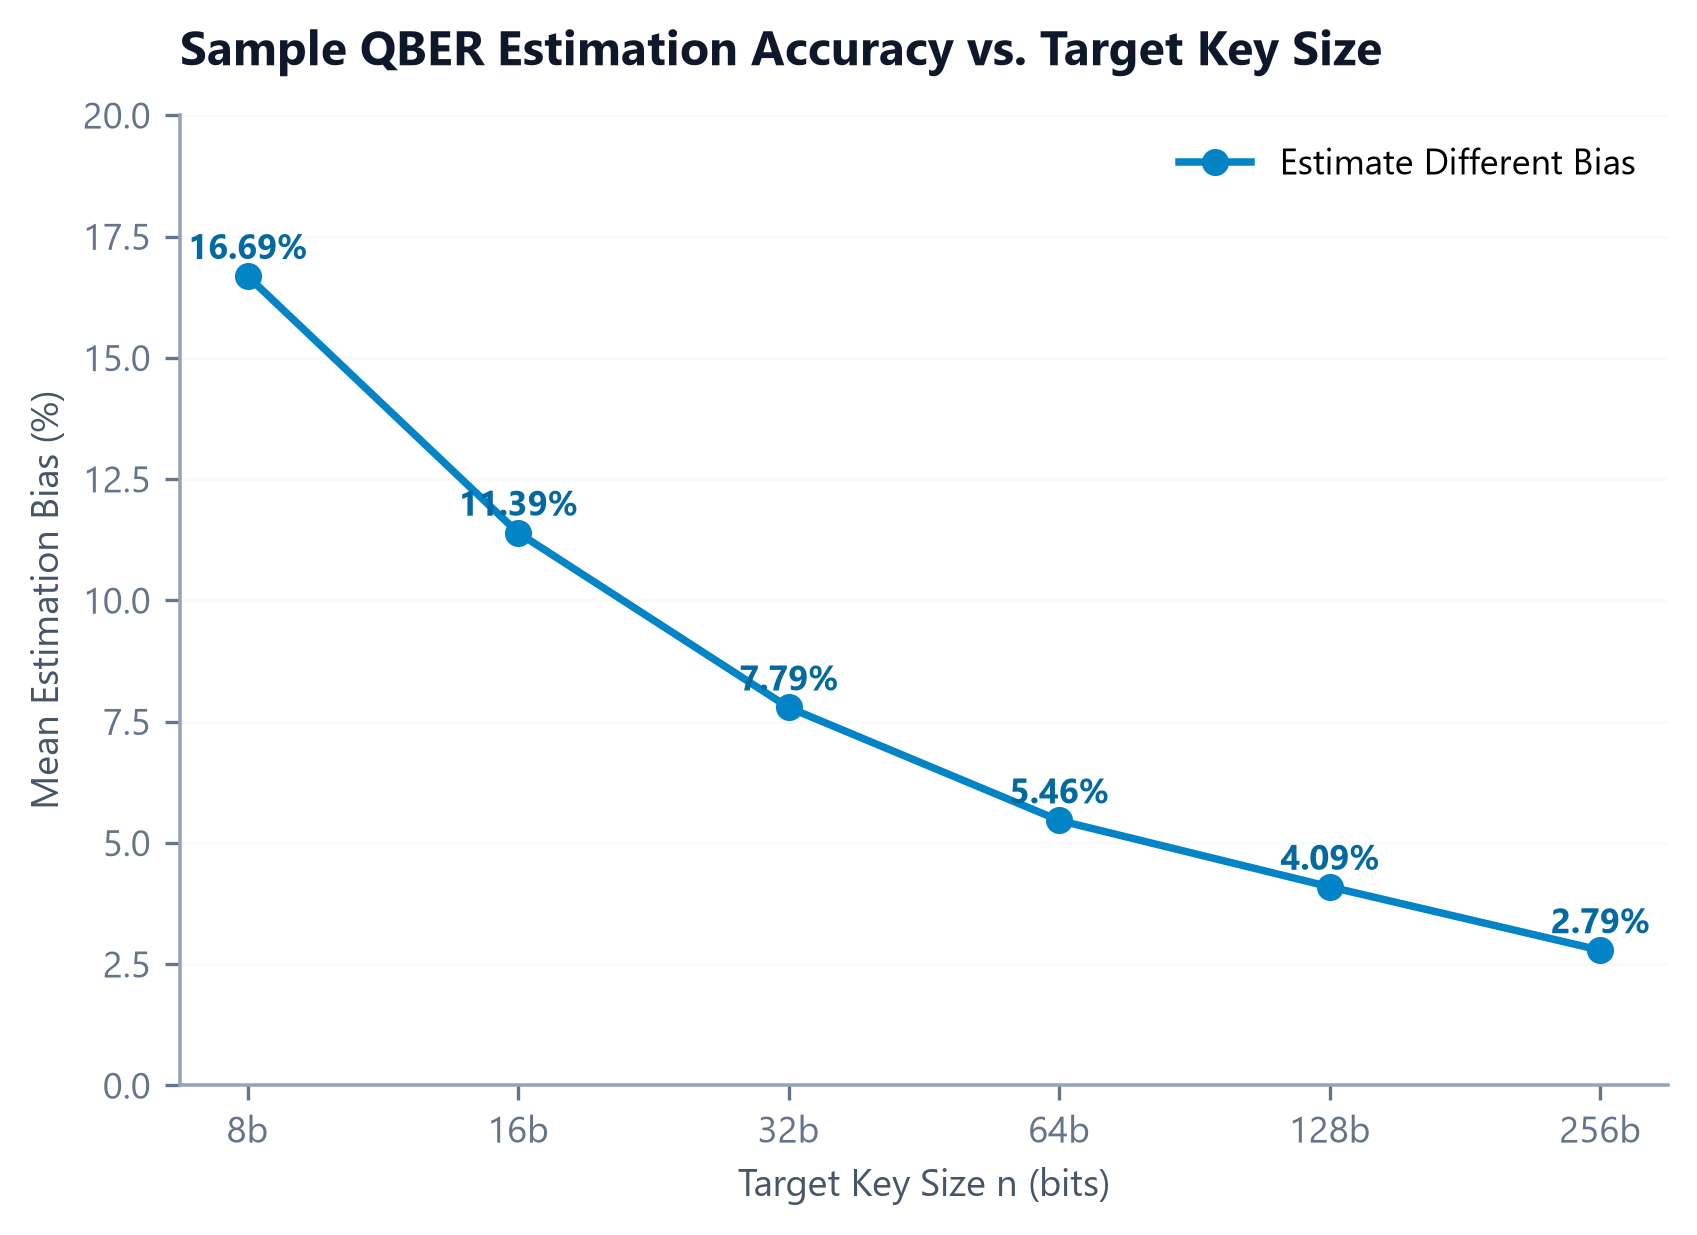
\includegraphics[width=0.75\textwidth]{figures/minimal_priority2_estimation_error_vs_keysize.png}
    \caption{ความคลาดเคลื่อนเฉลี่ยของ QBER เทียบกับขนาดกุญแจเป้าหมายบน IBM Quantum Hardware}
    \label{fig:estimation_bias}
\end{figure}

จากรูปที่~\ref{fig:estimation_bias} ยืนยันว่า ค่าความคลาดเคลื่อนเฉลี่ยมีแนวโน้มลดลงสอดคล้องกับ Law of Large Numbers โดยลดลงจาก $16.69\%$ ที่ $n = 8$ บิต ลงมาเหลือเพียง $5.46\%$ ที่ $n = 64$ บิต และต่ำสุดที่ $2.79\%$ ที่ $n = 256$ บิต ซึ่งแสดงให้เห็นว่า เมื่อขนาดกุญแจเพิ่มขึ้น จำนวนบิตกลุ่มตัวอย่างจะมากพอที่จะทำหน้าที่เป็นตัวแทนตรวจจับร่องรอยของผู้ดักฟังแทนกุญแจจริงได้อย่างเที่ยงตรงบนฮาร์ดแวร์จริง

\clearpage
\section{การทดลองที่ 3: การเปรียบเทียบข้อมูลที่ผู้ดักฟังล่วงรู้ก่อนและหลังการขยายความลับ (Privacy Amplification Evaluation)}

ในกรณีที่ผู้ดักฟังแอบดักฟังเพียงปริมาณน้อยจนค่า QBER ไม่เกินเกณฑ์ $11.0\%$ ผู้ดักฟังอาจล่วงรู้ข้อมูลบางบิตของกุญแจลับได้ ระบบจึงต้องทำ Privacy Amplification ด้วยการคูณเมทริกซ์โทพลิตซ์ (Toeplitz Hashing)~\cite{bennett_privacy_amp_1995, krawczyk_toeplitz} เพื่อบีบอัดกุญแจลับ การทดลองที่ 3 จึงทำการวัดปริมาณข้อมูลที่ผู้ดักฟังล่วงรู้ก่อนและหลังการทำ Hashing โดยแปรผันพารามิเตอร์ความปลอดภัย $s \in \{8, 16, 32\}$ บิต

ผลการประเมินแสดงในรูปที่~\ref{fig:privacy_amp_summary}

\begin{figure}[htbp]
    \centering
    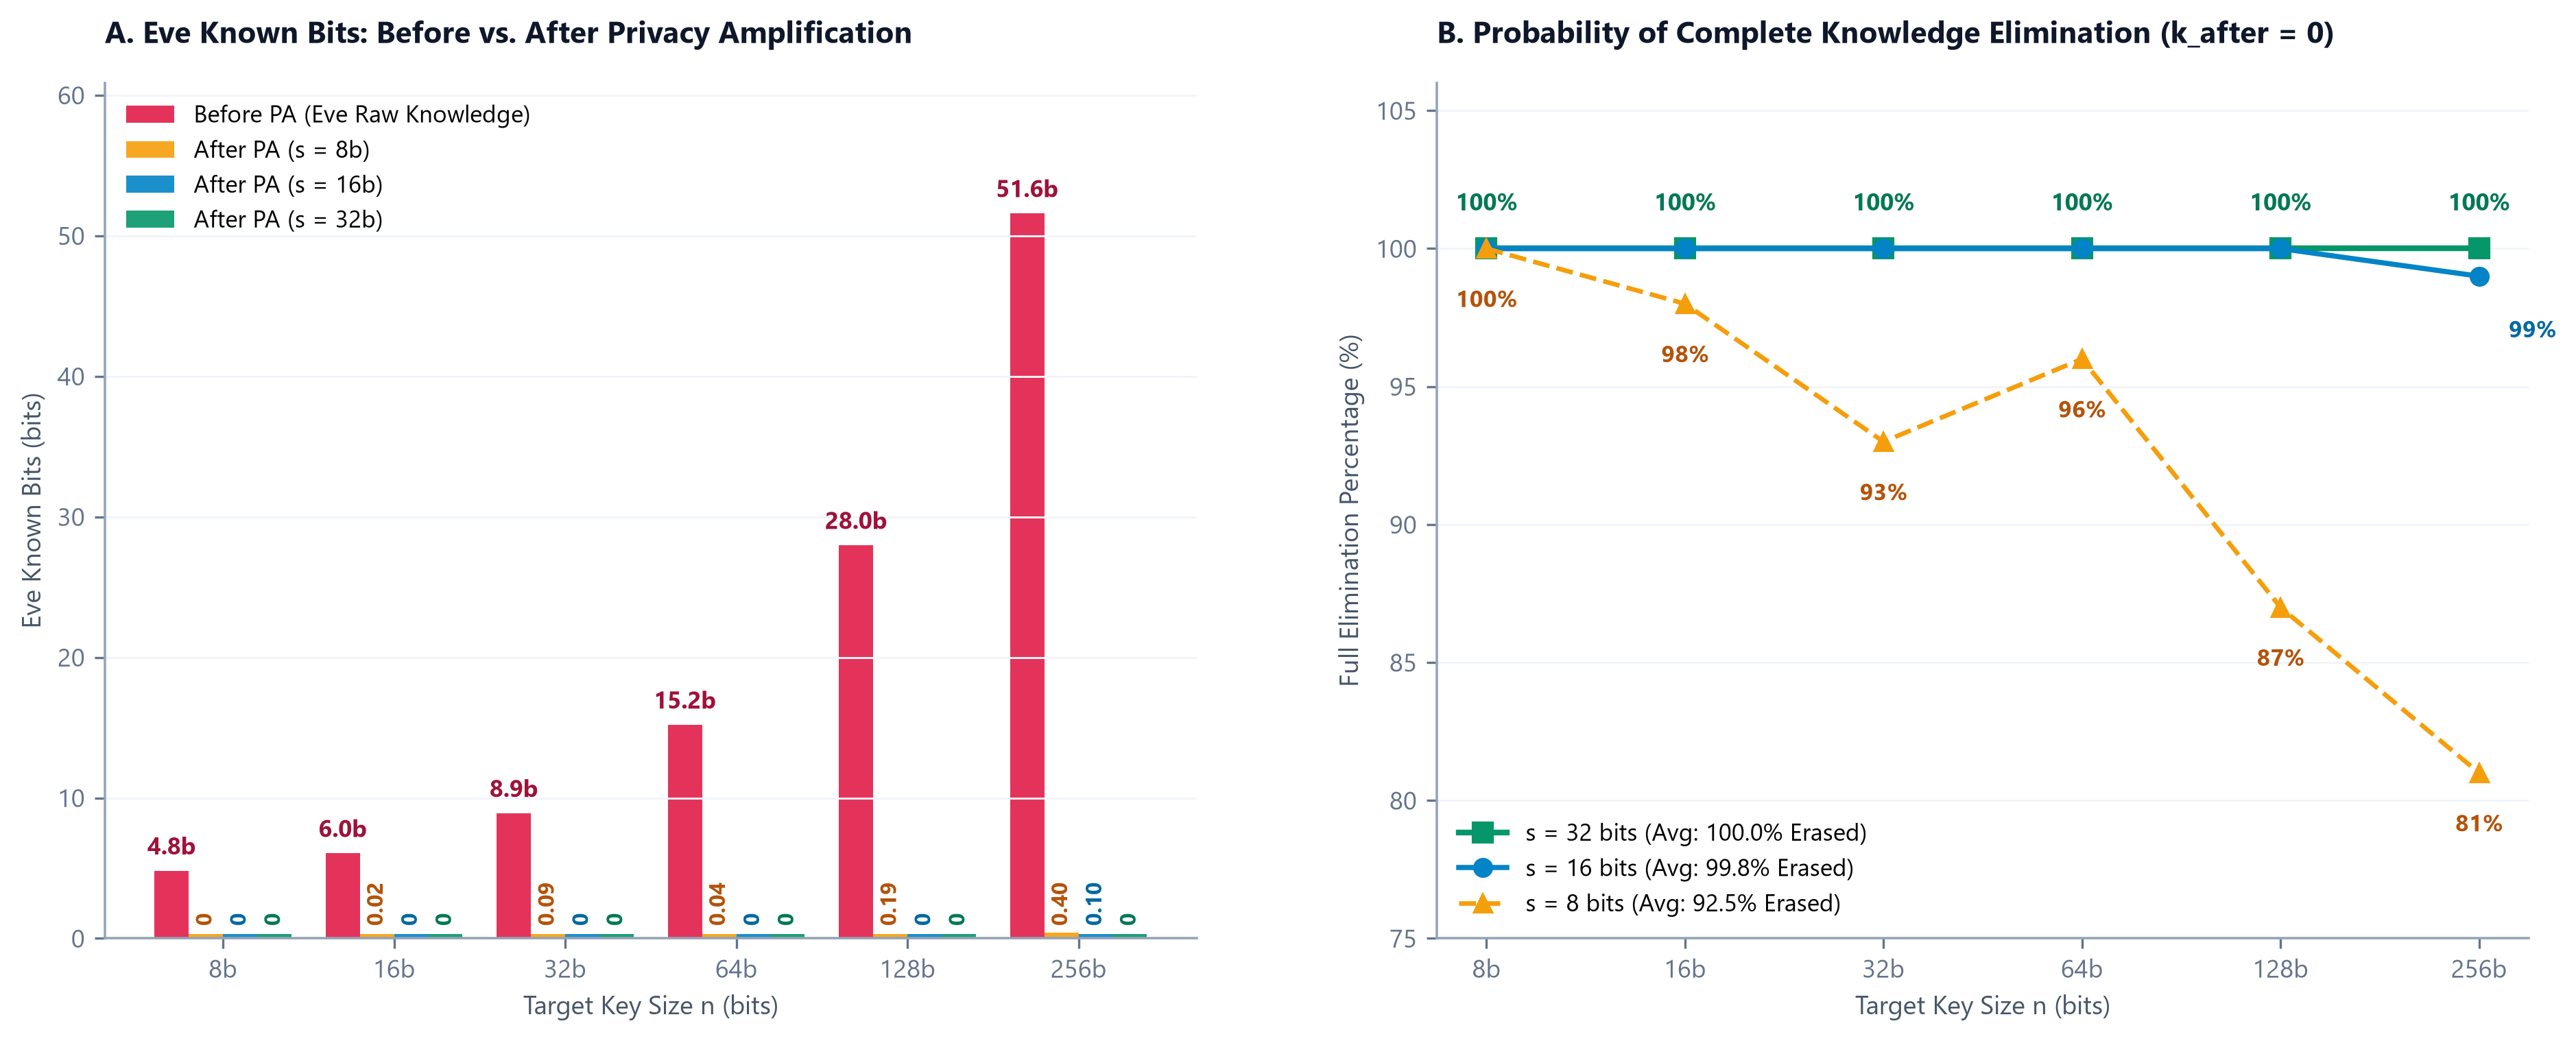
\includegraphics[width=0.92\textwidth]{figures/minimal_privacy_amplification_summary.png}
    \caption{ผลการประเมินกระบวนการ Privacy Amplification: (A) จำนวนบิตที่ผู้ดักฟังล่วงรู้ก่อนและหลังบีบอัด และ (B) ความน่าจะเป็นในการทำลายความรู้ของผู้ดักฟังได้อย่างสมบูรณ์ ($k_{\text{after}} = 0$)}
    \label{fig:privacy_amp_summary}
\end{figure}



จากรูปที่~\ref{fig:privacy_amp_summary} พบว่า:
\begin{enumerate}
    \item \textbf{หลังทำ Hashing (After PA):} เมื่อใช้พารามิเตอร์ความปลอดภัย $s \ge 16$ บิต ปริมาณข้อมูลของผู้ดักฟังจะลดลงเหลือ $0.00$ บิตในเกือบทุกขนาดกุญแจ โดยมีอัตราการกำจัดความรู้ของผู้ดักฟังโดยสมบูรณ์ ($k_{\text{after}} = 0$) อยู่ที่ $99\% - 100\%$ และเมื่อใช้ $s = 32$ บิตจะได้ $100\%$ ทุกขนาดกุญแจ
    \item \textbf{การเลือกค่าพารามิเตอร์ $s$:} หากใช้ $s = 8$ บิต อัตราการกำจัดข้อมูลสมบูรณ์จะลดลงเหลือ $87\%$ และ $81\%$ ที่คีย์ขนาด $128$ และ $256$ บิตตามลำดับ ดังนั้นการเลือกใช้ $s \ge 16$ บิตจึงเป็นเกณฑ์ที่ปลอดภัยสำหรับการใช้งานจริง
\end{enumerate}

\clearpage
\section{การอภิปรายผลการทดลองและข้อจำกัดของระบบ}

ผลการทดลองทั้ง 3 ส่วนข้างต้นพิสูจน์ให้เห็นถึงประสิทธิภาพของโพรโทคอล BB84 ร่วมกับ One-Time Pad บนคอมพิวเตอร์ควอนตัมจริง อย่างไรก็ตาม เมื่อพิจารณาในบริบทของการนำไปประยุกต์ใช้งานเชิงปฏิบัติการ ยังคงมีข้อจำกัดทางกายภาพสำคัญ 4 ประการที่ค้นพบจากการทดลองบนฮาร์ดแวร์จริง:

\begin{enumerate}
    \item \textbf{สัญญาณรบกวนทางกายภาพ:} อนุภาคควอนตัมบนฮาร์ดแวร์จริงมีความเปราะบางสูง ทำให้เกิด Error พื้นฐานจากเกตควอนตัมและการรักษาสภาพสถานะทางควอนตัม $2\% - 3\%$ แม้ไม่มีการดักฟัง จึงต้องอาศัยการตั้งค่าเกณฑ์ความปลอดภัยที่รัดกุมเพื่อให้ระบบยังคงทำงานได้และยังมีความปลอดภัย
    \item \textbf{ข้อจำกัดจำนวนคิวบิตและการเชื่อมต่อกุญแจหลายรอบ:} คอมพิวเตอร์ควอนตัมจริงในปัจจุบันมีจำนวนคิวบิตที่ใช้งานได้พร้อมกันจำนวนจำกัด และการรอจองคิวบิตจำนวนมากพร้อมกันต้องใช้เวลารอนาน ทำให้การสร้างกุญแจในครั้งเดียวไม่สามารถสร้างกุญแจขนาดยาวได้ ระบบจึงต้องใช้การแบ่งสร้างกุญแจเป็นรอบย่อยแล้วเชื่อมต่อกันหลายรอบ
    \item \textbf{ระยะทางของช่องสัญญาณควอนตัม:} การส่งสัญญาณแสงโฟตอนผ่านสายใยแก้วนำแสงในโลกความเป็นจริงจะเกิดการลดทอนสัญญาณลงอย่างรวดเร็ว และจาก No-Cloning Theorem ทำให้ไม่สามารถใช้เครื่องขยายสัญญาณแบบดั้งเดิมได้ ส่งผลให้ระยะการส่งจำกัดอยู่ในระดับไม่เกิน 50--100 กิโลเมตร
    \item \textbf{ข้อจำกัดด้านความเป็นนิรนาม:} ในการเข้ารหัสแบบ One-Time Pad ระหว่าง Voter และ Server เครื่องเซิร์ฟเวอร์จำเป็นต้องทราบว่ากุญแจแต่ละชุดเป็นของผู้ลงคะแนนคนใดเพื่อใช้ในการถอดรหัสผลโหวต ส่งผลให้เซิร์ฟเวอร์สามารถล่วงรู้ความสัมพันธ์ระหว่างตัวตนกับข้อความโหวตได้ ซึ่งโครงงานนี้มุ่งเน้นการส่งกุญแจให้ปลอดภัยจากการโจมตีเชิงควอนตัมเป็นหลัก
\end{enumerate}

\section{สรุปผลการทดสอบ}

การทดลองและประเมินผลบนฮาร์ดแวร์ประมวลผลควอนตัมจริงของ IBM Quantum ในบทนี้ สรุปข้อค้นพบสำคัญได้ดังนี้:
\begin{itemize}
    \item การทดสอบบน IBM Quantum Hardware ยืนยันว่าระบบสามารถตรวจจับการดักฟังได้ด้วยความแม่นยำ $100.0\%$ เมื่อกุญแจมีขนาดตั้งแต่ $32$ บิตขึ้นไป แม้จะมีสัญญาณรบกวนปะปนอยู่
    \item บิตกลุ่มตัวอย่างมีความคลาดเคลื่อนเฉลี่ยต่ำเพียง $2.79\%$ (ที่ $n = 256$ บิต) ซึ่งสามารถใช้เป็นค่าตัวแทนตรวจวัด QBER ของกุญแจลับจริงได้
    \item กระบวนการ Privacy Amplification ด้วย Toeplitz Hashing สามารถทำลายข้อมูลที่ผู้ดักฟังแอบล่วงรู้ได้อย่างเบ็ดเสร็จ ($99\% - 100\%$ ที่ $s = 16$ และ $100\%$ ที่ $s = 32$)
\end{itemize}

\ifproject
% !TEX root = ../main.tex
\chapter{\ifenglish Conclusions and Discussions\else บทสรุปและข้อเสนอแนะ\fi}

ในบทนี้สรุปผลการดำเนินงานของโครงงานระบบการสื่อสารความปลอดภัยสูงสำหรับการลงคะแนนเสียงโดยใช้การกระจายกุญแจแบบควอนตัม (BB84 QKD) ทั้งในด้านความสำเร็จตามวัตถุประสงค์ ผลการทดสอบบนฮาร์ดแวร์จริงของ IBM Quantum ปัญหาอุปสรรคพร้อมแนวทางแก้ไขเชิงวิศวกรรม ข้อจำกัด และข้อเสนอแนะสำหรับการพัฒนาต่อยอด

\section{\ifenglish Conclusions\else สรุปผลการดำเนินงาน\fi}

โครงงานได้ออกแบบ พัฒนา และทดสอบระบบการลงคะแนนเสียงอิเล็กทรอนิกส์ที่มีปลอดภัยแบบ Information-Theoretic Security โดยนำโพรโทคอล BB84 ร่วมกับการเข้ารหัส One-Time Pad (OTP) มาประยุกต์ใช้ในช่องทางการส่งบัตรลงคะแนน โดยมีผลสัมฤทธิ์หลักตามวัตถุประสงค์ดังนี้:

\begin{enumerate}
    \item \textbf{กระบวนการความปลอดภัยของระบบ:} พัฒนาระบบตั้งแต่การสร้างวงจรควอนตัมใน Z-basis และ X-basis, การเปรียบเทียบแกน (Basis Sifting), การประเมินค่า QBER จากบิตทดสอบ, การตรวจจับผู้ดักฟัง, การขยายความปลอดภัยด้วยเมทริกซ์โทพลิตซ์ (Privacy Amplification) และการเข้ารหัสบัตรลงคะแนนด้วย One-Time Pad ($C = M \oplus K$) ได้อย่างสมบูรณ์
    
    \item \textbf{การทดสอบบนฮาร์ดแวร์ IBM Quantum จริง:} ผลการทดสอบบนชิปประมวลผลควอนตัมยืนยันประสิทธิภาพของระบบ 3 ประการ:
    \begin{itemize}
        \item \textit{การตรวจจับการดักฟัง:} ตรวจจับการดักฟังแบบ Intercept-and-Resend ได้แม่นยำ $100.0\%$ ปราศจาก False Alarm เมื่อขนาดกุญแจ $n \ge 32$ บิต
        \item \textit{ความเที่ยงตรงของบิตกลุ่มตัวอย่าง:} ค่าความคลาดเคลื่อนเฉลี่ยในการประมาณการ QBER ลดลงตามกฎจำนวนมาก จาก $16.69\%$ ที่ $n = 8$ บิต เหลือเพียง $2.79\%$ ที่ $n = 256$ บิต
        \item \textit{การกำจัดข้อมูลรั่วไหล:} กระบวนการ Privacy Amplification ด้วยค่าความปลอดภัย $s \ge 16$ บิต สามารถลดข้อมูลที่ผู้ดักฟังล่วงรู้ได้เกือบทั้งหมด (ความสำเร็จ $99\% - 100\%$)
    \end{itemize}

    \item \textbf{เว็บแอปพลิเคชันเชิงโต้ตอบ:} พัฒนาระบบส่วนต่อประสาน 3 มุมมอง (Voter View, Practical View, และ System God View) ช่วยให้สังเกตและตรวจสอบการทำงานของวงจรควอนตัมและสถานะความปลอดภัยได้อย่างชัดเจน
\end{enumerate}

\subsection{ข้อจำกัดของระบบที่ค้นพบจากการทดลอง}

\begin{itemize}
    \item \textbf{ความเป็นนิรนาม (Anonymity Trade-off):} การถอดรหัสแบบ One-Time Pad ฝั่งผู้รับ (Server) จำเป็นต้องจับคู่กุญแจกับผู้ลงคะแนน ($M = C \oplus K$) เซิร์ฟเวอร์จึงยังล่วงรู้ความสัมพันธ์ระหว่างผู้ลงคะแนนกับบัตรเลือกตั้งได้ ซึ่งต้องใช้กลไกไม่เปิดเผยตัวตนในระดับแอปพลิเคชันเพิ่มเติมหากต้องการความเป็นนิรนามขั้นสูงสุด
    \item \textbf{การไม่มีกลไกแก้ไขข้อผิดพลาด (No Error Correction):} ระบบอาศัยการยกเลิกเซสชัน (Abort) ทันทีที่ QBER เกินเพดาน $11.0\%$ โดยไม่มีโพรโทคอลแก้ไขข้อผิดพลาดทางคลาสสิก (เช่น Cascade หรือ LDPC) ทำให้ประสิทธิภาพขึ้นอยู่กับคุณภาพของชิปควอนตัมโดยตรง
    \item \textbf{ระยะทางของช่องสัญญาณกายภาพ:} ในสายใยแก้วนำแสงจริง อนุภาคโฟตอนเดี่ยวจะเกิดการลดทอนสัญญาณตามระยะทาง (Attenuation) จำกัดระยะการเชื่อมต่อระหว่างหน่วยเลือกตั้งกับศูนย์กลางไว้ที่ไม่เกิน 50--100 กิโลเมตร
\end{itemize}

\section{\ifenglish Challenges and Engineering Solutions\else ปัญหาที่พบและแนวทางการแก้ไขเชิงวิศวกรรม\fi}

ในการพัฒนาและทดสอบระบบบนฮาร์ดแวร์ประมวลผลควอนตัมจริง พบความท้าทายทางวิศวกรรมและมีแนวทางแก้ไข 4 ประการ:

\begin{enumerate}
    \item \textbf{การจำแนกสัญญาณรบกวนฮาร์ดแวร์ออกจากการดักฟัง:} สัญญาณรบกวนทางกายภาพของฮาร์ดแวร์จริง ($2.0\% - 3.0\%$) อาจกระตุ้นให้ระบบแจ้งเตือนเท็จ โครงงานแก้ปัญหานี้โดยกำหนดเกณฑ์เพดาน $QBER_{\text{threshold}} = 11.0\%$ ตามบทพิสูจน์ของ Shor และ Preskill ซึ่งสร้างส่วนต่างความปลอดภัย (Safety Margin) กว้าง $\approx 8.5\%$ เหนือสัญญาณรบกวน ทำให้สามารถจำแนกการดักฟังแบบ Intercept-and-Resend ($\approx 25\%$) ได้แม่นยำ $100\%$ โดยไม่มีการแจ้งเตือนเท็จ
    
    \item \textbf{ข้อจำกัดจำนวนคิวบิตและเวลารอคิวบนคลาวด์ควอนตัม:} การสร้างกุญแจยาวในรอบเดียวทำได้ยากเนื่องจากข้อจำกัดคิวบิตและเวลารอคิว จึงพัฒนาเทคนิค \textbf{Multi-Session Key Concatenation} โดยแบ่งการสร้างกุญแจออกเป็นรอบย่อยขนาด 20--40 คิวบิต แล้วนำกุญแจที่ผ่านการตรวจสอบมาเชื่อมต่อกันจนครบความยาวเป้าหมาย ซึ่งใช้รอบย่อยเฉลี่ยเพียง $3.2$ รอบสำหรับกุญแจ 24 บิต
    
    \item \textbf{ความแปรปรวนทางสถิติในกุญแจขนาดเล็ก:} ที่ขนาดกุญแจสั้น ($n = 8$ บิต) บิตกลุ่มตัวอย่างมีน้อย (9 บิต) ทำให้เกิดความผันผวนทางสถิติจนเกิด False Alarm $7\%$ และมีอัตราหลุดรอด $10\%$ จึงกำหนดข้อกำหนดทางวิศวกรรมให้ $n \ge 32$ บิตขึ้นไป (กลุ่มตัวอย่าง $\ge 38$ บิต) ซึ่งลดความคลาดเคลื่อนเฉลี่ยต่ำกว่า $7.8\%$ และขจัดความผิดพลาดทั้งสองส่วนเหลือ $0.0\%$
    
    \item \textbf{การรั่วไหลของข้อมูลในการดักฟังแบบแอบแฝง (Sub-Threshold):} หากผู้ดักฟังดักข้อมูลเพียงบางส่วนเพื่อให้ QBER ไม่เกิน $11.0\%$ ผู้ดักฟังอาจได้ข้อมูลกุญแจดิบไปบางส่วน ($4.8$ ถึง $51.6$ บิต) โครงงานแก้ปัญหาโดยใช้ Toeplitz Universal Hashing บน $\text{GF}(2)$ ด้วยค่าพารามิเตอร์ $s \ge 16$ บิต ซึ่งบีบอัดและทำลายข้อมูลรั่วไหลจนผู้ดักฟังมีความรู้หลังการบีบอัดเป็น $0.00$ บิตอย่างแน่นอน
\end{enumerate}

\section{\ifenglish Suggestions and Future Work\else ข้อเสนอแนะและแนวทางการพัฒนาต่อ\fi}

แนวทางการวิจัยและพัฒนาต่อยอดเพื่อยกระดับสู่การใช้งานจริงในอนาคต ประกอบด้วย 4 มิติ:

\begin{enumerate}
    \item \textbf{การยกระดับความเป็นนิรนามขั้นสูง:} ประยุกต์ใช้เทคนิคทางวิทยาการรหัสลับสมัยใหม่ เช่น เครือข่ายสับเปลี่ยนบัตรลงคะแนน (Mix-nets) หรือการพิสูจน์แบบความรู้เป็นศูนย์ (Zero-Knowledge Proofs: ZKP) เพื่อตัดความสัมพันธ์ระหว่างตัวตนผู้ลงคะแนนกับบัตรเลือกตั้งในระดับแอปพลิเคชัน
    
    \item \textbf{การผสานอัลกอริทึมแก้ไขข้อผิดพลาดทางคลาสสิก:} ผสานรวม Cascade Protocol หรือ Low-Density Parity-Check (LDPC) Codes ในขั้นตอน Classical Post-Processing เพื่อกู้คืนบิตที่ผิดพลาดจากสัญญาณรบกวนโดยไม่ต้องทำลายกุญแจทิ้ง ช่วยเพิ่มอัตราการสร้างกุญแจสำเร็จ (Key Generation Rate)
    
    \item \textbf{การทดสอบบนโครงข่ายใยแก้วนำแสงจริง:} นำระบบไปเชื่อมต่อกับฮาร์ดแวร์โฟโตนิกส์จริง ได้แก่ เลเซอร์พัลส์อ่อน ตัวปรับมุมโพลาไรเซชัน สายไฟเบอร์ออปติก Single-Mode และตัวตรวจวัดโฟตอนเดี่ยว (SPADs) เพื่อประเมินผลกระทบของการลดทอนสัญญาณจริง
    
    \item \textbf{สถาปัตยกรรมความปลอดภัยแบบลูกผสม (Hybrid QKD + PQC):} นำวิทยาการรหัสลับยุคหลังควอนตัมตามมาตรฐาน NIST เช่น ML-DSA (Dilithium) มาใช้ยืนยันตัวตนคู่สื่อสารบนช่องทางคลาสสิก เพื่อป้องกันการโจมตีแบบสวมรอยเป็นคนกลาง (Man-in-the-Middle) และใช้ ML-KEM (Kyber) ร่วมกับ QKD เพื่อสร้างการป้องกันแบบหลายชั้น (Defense-in-Depth)
\end{enumerate}

\fi

\bibliography{sampleReport}

\ifproject
\normalspacing
\appendix
% !TEX root = ../main.tex
\chapter{\ifenglish Manual\else คู่มือการใช้งานระบบ\fi}

เนื้อหาคู่มือการใช้งานระบบเว็บแอปพลิเคชันจำลองการโหวตด้วยโพรโทคอล BB84 และ One-Time Pad


%% Display glossary (optional) -- need glossary option.
\ifglossary\glossarypage\fi

%% Display index (optional) -- need idx option.
\ifindex\indexpage\fi

\begin{biosketch}
% รูปผู้เขียน: วางไฟล์ที่ figures/author_<ชื่อ>.jpg ถ้ายังไม่มีไฟล์จะแสดงกรอบว่างแทน
\newcommand{\authorphoto}[1]{%
  \IfFileExists{#1}{\includegraphics[width=1.2in,height=1.5in,keepaspectratio]{#1}}%
  {\fbox{\parbox[c][1.5in][c]{1.2in}{\centering\small รูปถ่าย}}}}
\newcommand{\authorbio}[5]{%
  \begin{center}\authorphoto{#1}\end{center}
  \begin{tabular}{@{}l@{\quad}p{0.7\textwidth}@{}}
    \textbf{ชื่อ-นามสกุล} & #2 \\
    \textbf{รหัสนักศึกษา} & #3 \\
    \textbf{การศึกษา} & #4 \\
    \textbf{อีเมล} & \texttt{#5}
  \end{tabular}\par\bigskip}

\authorbio{figures/author_pakin.jpg}{นายภคิน นิรมิตสีมา}{660610782}
  {ปริญญาตรี สาขาวิศวกรรมคอมพิวเตอร์ คณะวิศวกรรมศาสตร์ มหาวิทยาลัยเชียงใหม่}
  {pakin\_ni@cmu.ac.th}

\authorbio{figures/author_yuttakan.jpg}{นายยุทธกานต์ สาจุ้ย}{660610787}
  {ปริญญาตรี สาขาวิศวกรรมคอมพิวเตอร์ คณะวิศวกรรมศาสตร์ มหาวิทยาลัยเชียงใหม่}
  {gong6321@gmail.com}

\authorbio{figures/author_atinan.jpg}{นายอาทินันท์ แจ้งสว่าง}{660610807}
  {ปริญญาตรี สาขาวิศวกรรมคอมพิวเตอร์ คณะวิศวกรรมศาสตร์ มหาวิทยาลัยเชียงใหม่}
  {atinanhome@gmail.com}

\authorbio{figures/author_paisit.jpg}{นายไพสิฐ เลิศอนันต์พิพัฒน์}{660612155}
  {ปริญญาตรี สาขาวิศวกรรมคอมพิวเตอร์ คณะวิศวกรรมศาสตร์ มหาวิทยาลัยเชียงใหม่}
  {paisitture@gmail.com}
\end{biosketch}
\fi % \ifproject
\end{document}
